% Arquivo Principal para Dissertações do PPGCA - Udesc Joinville

% abnTeX2: Modelo de Trabalho Academico em conformidade com
% ABNT NBR 14724:2011: Informacao e documentacao - Trabalhos academicos -
% Apresentacao

% Adaptado com base no abnTeX2
% Por: Luís Felipe Bilecki
% E-mail: luis.bilecki@gmail.com
% ------------------------------------------------------------------------
% ------------------------------------------------------------------------
\documentclass[
	12pt,				% tamanho da fonte
	openright,			% capítulos começam em pág ímpar (insere página vazia caso preciso)
	oneside,
	a4paper,			% tamanho do papel.
	chapter=TITLE,		% títulos de capítulos convertidos em letras maiúsculas
	section=TITLE,		% títulos de seções convertidos em letras maiúsculas
	%subsection=TITLE,	% títulos de subseções convertidos em letras maiúsculas
	%subsubsection=TITLE,% títulos de subsubseções convertidos em letras maiúsculas
	% -- opções do pacote babel --
	english,			% idioma adicional para hifenização
	brazil,				% o último idioma é o principal do documento
  hidelinks
	]{abntex2}

%Pacotes prinicipais e customização
\usepackage{./Estilo/udesc}

% ---
% Dados da Capa
% ---

\titulo{SISTEMA DE RECOMENDAÇÃO SENSÍVEL AO TEMPO EM AMBIENTES VIRTUAIS DE APRENDIZAGEM}
\autor{EDUARDO JOSÉ DE BORBA}
\local{Joinville}
\instituicao{Universidade do Estado de Santa Catarina - UDESC}
\campus{Centro de Ciências Tecnológicas - CCT}
\curso{Mestrado em Computação Aplicada}
\data{2017}
\fulldata{11 de Dezembro de 2017}

% ---
% Folha de Rosto
% ---
\inforosto{Qualificação apresentada ao Programa de Pós-Graduação em Computação Aplicada, da Universidade do Estado de Santa
    Catarina, como requisito parcial para a obtenção do grau de Mestre em Computação Aplicada.}
\orientador{Isabela Gasparini}
\orientadorRotulo{Dra. }
\coorientador{Daniel Lichtnow}
\coorientadorRotulo{Dr. }

% ----
% Início do documento
% ----
\begin{document}
% ----
% Elementos Pré-Textuais
% ----
%!TEX root = ../Principal.tex
%Capa do Trabalho
\imprimircapa

%Folha de Rosto
%* indica que tem ficha catalográfica
\imprimirfolhaderosto*

% ---
% Caso a Biblioteca da UDESC forneça, utilize o comando
% ---
% \begin{fichacatalografica}
%     \includepdf{fig_ficha_catalografica.pdf}
% \end{fichacatalografica}

% ---
% Geração da Ficha Catalográfica Via LaTeX
% ---
% \begin{fichacatalografica}
% 	\vspace*{\fill}					% Posição vertical
% 	\begin{center}					% Minipage Centralizado
% 	\begin{minipage}[c]{12.5cm}		% Largura

% 	\imprimirautor

% 	\hspace{0.5cm} \imprimirtitulo  / \imprimirautor. --
% 	\imprimirlocal, \imprimirdata-

% 	\hspace{0.5cm} \pageref{LastPage} p. : il. (algumas color.) ; 30 cm.\\

% 	\hspace{0.5cm} \imprimirorientadorRotulo~\imprimirorientador\\

% 	\hspace{0.5cm}
% 	\parbox[t]{\textwidth}{\imprimirtipotrabalho~--~\imprimirinstituicao,
% 	\imprimirdata.}\\

% 	\hspace{0.5cm}
% 		1. Tópico 01.
% 		2. Tópico 02.
% 		I. Prof. Dr. xxxxx.
% 		II. Universidade do Estado de Santa Catarina.
% 		III. Centro de Ciências Tecnológicas.
% 		IV. identificação xxxx\\

% 	\hspace{8.75cm} CDU 02:121:005.7\\

% 	\end{minipage}
% 	\end{center}
% \end{fichacatalografica}

% % ---
% % Folha de Aprovação
% % ---
% % Exemplo de folha de aprovação antes da Banca. Após isso, incluia o pdf digitalizado com as assinaturas%
% % 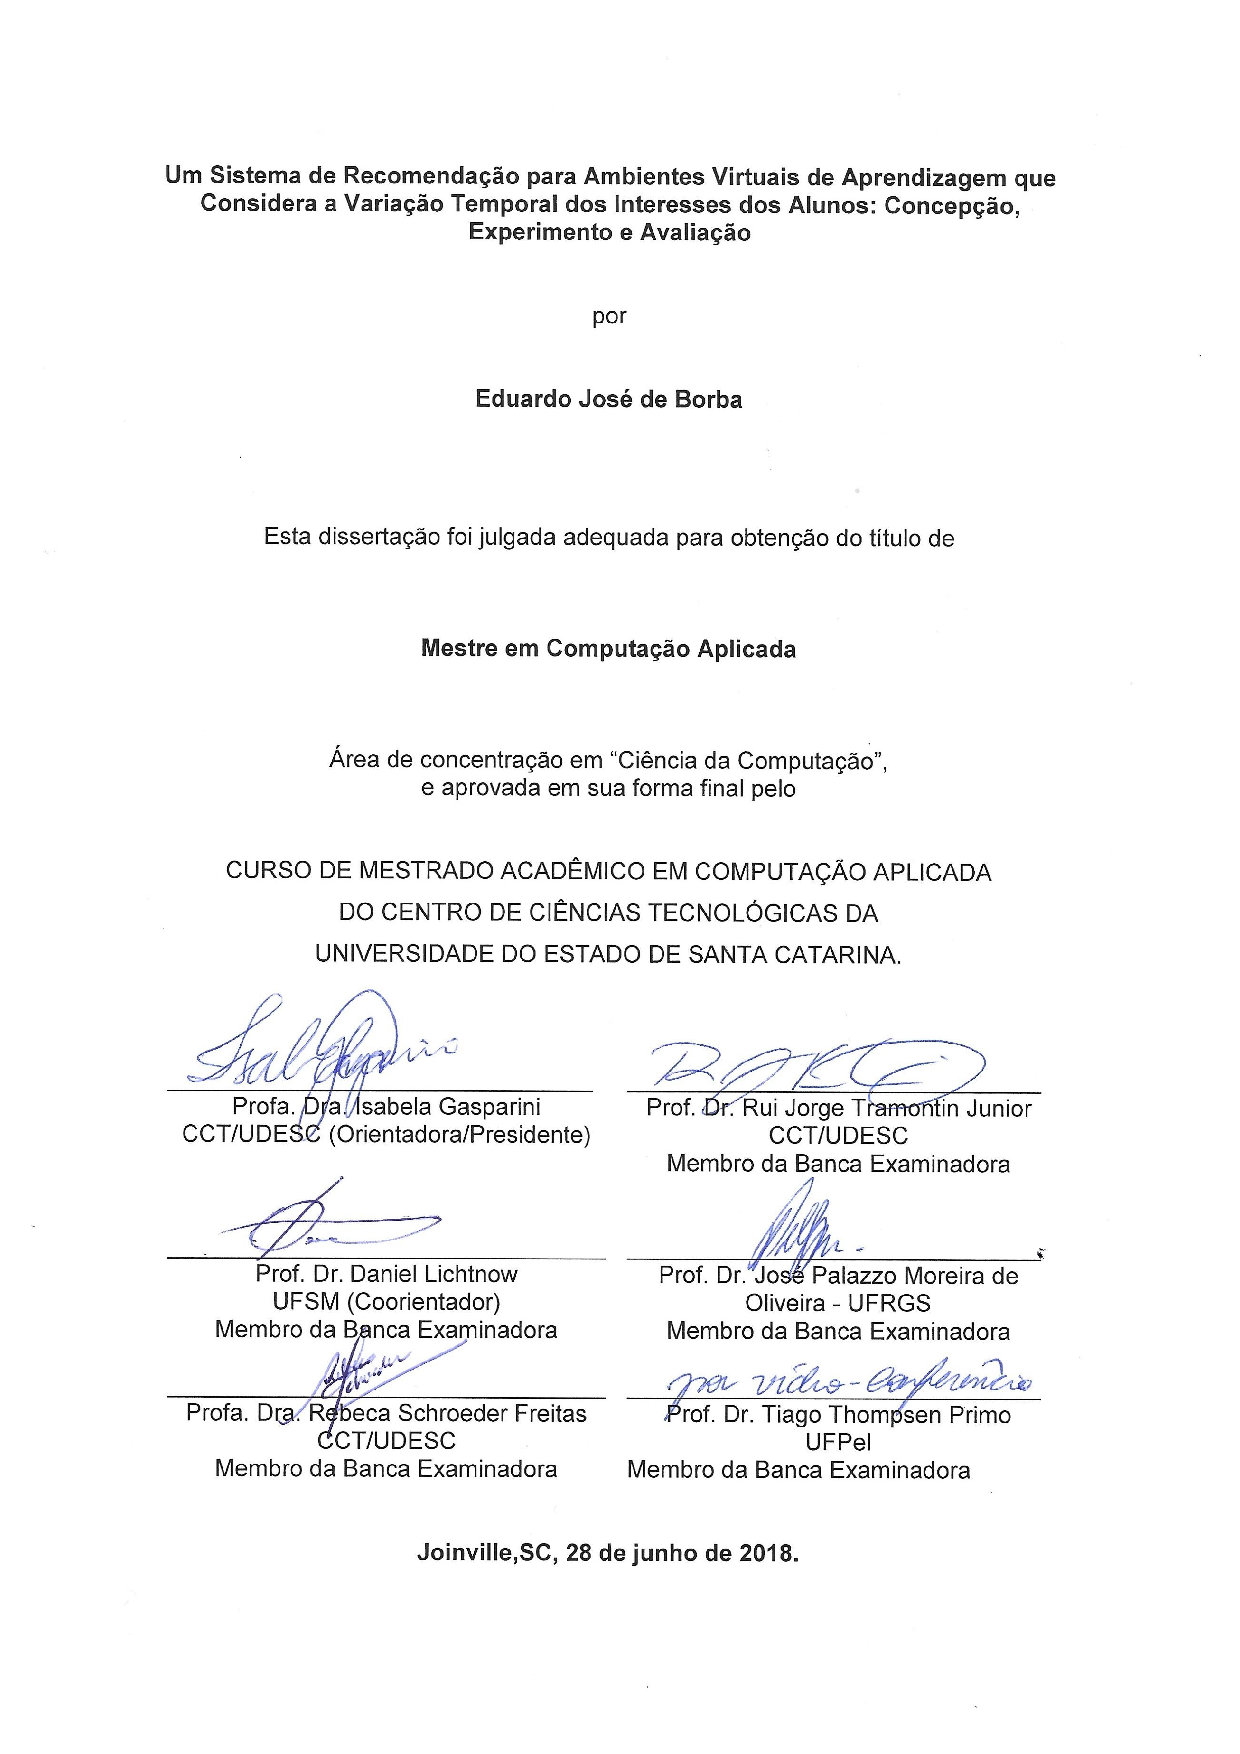
\includepdf{folhadeaprovacao_final.pdf}
\begin{folhadeaprovacao}
	\begin{center}
		{\ABNTEXchapterfont\bfseries\imprimirautor}
		\vspace{2em}

			\ABNTEXchapterfont\bfseries\imprimirtitulo

	\end{center}
		\vspace{1em}
		{\justify
    Dissertação apresentada ao Programa de Pós-Graduação em Computação Aplicada, da Universidade do Estado de Santa
    Catarina, como requisito parcial para a obtenção do grau de Mestre em Computação Aplicada.}
	 \vspace{2em}
	\noindent

	{\justify \bfseries Banca Examinadora}

  \vspace{2em}

  \noindent{Orientadora:\hfill \assinatura*{\textbf{\imprimirorientadorRotulo \imprimirorientador} \\ Universidade do Estado de Santa Catarina (UDESC)}}

  \noindent{Coorientador:\hfill \assinatura*{\textbf{\imprimircoorientadorRotulo \imprimircoorientador} \\ Universidade Federal de Santa Marina (UFSM)}}

  \noindent{Membros:}

	\noindent{\assinatura*{\textbf{Dr. Rui Jorge Tramontin Junior} \\ Universidade do Estado de Santa Catarina (UDESC)}}
  \noindent{\assinatura*{\textbf{Dra. Rebeca Schroeder Freitas} \\ Universidade do Estado de Santa Catarina (UDESC)}}
  \noindent{\assinatura*{\textbf{Dr. Thiago T. Primo} \\ Universidade Federal de Pelotas (UFPel)}}
  \noindent{\assinatura*{\textbf{Dr. José Palazzo M. de Oliveira} \\ Universidade Federal do Rio Grande do Sul (UFRGS)}}

    \vspace*{\fill}
    \begin{center}
    	\imprimirlocal,\,\imprimirfulldata
    \end{center}
\end{folhadeaprovacao}

% ---
% Dedicatória
% ---
% \begin{dedicatoria}
% Dedico este trabalho aos meus familiares, amigos, colegas e professores que me acompanharam e me deram forças nessa magnífica trajetória.
% \end{dedicatoria}

% % ---
% % Agradecimentos
% % ---
% \begin{agradecimentos}
% Gostaria de agradecer...

% Aqui devem ser colocadas os agradecimentos às pessoas que de alguma forma contribuíram para a realização do trabalho.
% \end{agradecimentos}

% ---
% Epígrafe
% ---
% \begin{epigrafe}
% ``Independentemente das circunstâncias, devemos ser sempre humildes, recatados e despidos de orgulho.''
% \\
% \par
% Dalai Lama
% \end{epigrafe}

% ---
% RESUMOS
% ---

% Português
\begin{resumo}
  Sistemas de Recomendação (SR) são ferramentas de software que sugerem itens para os usuários de forma automatizada e personalizada,
  sem a necessidade do usuário formular uma consulta para encontrar os itens do seu interesse. Esses sistemas são
  explorados em Ambientes Virtuais de Aprendizagem (AVA) com o objetivo de reduzir alguns problemas existentes nesses ambientes
  quando a quantidade de materiais disponíveis é grande, tais como: sobrecarga cognitiva, dificuldade de encontrar os materiais
  do seu interesse e muitos materiais nunca serem utilizados. Pesquisadores da área argumentam que os algoritmos de SRs tradicionais não são suficientes para os AVAs,
  sendo necessário um nível maior de personalização a situação do usuário, como considerar dimensões do contexto. O objetivo
  desse trabalho é a criação de perfis de usuário que levem em conta a mudança dos interesses destes usuários
  ao longo do tempo. O algoritmo proposto combina a (1) similaridade do perfil do usuário (representado
  pelos materiais acessados pelo usuário) com os itens disponíveis para a recomendação com a (2) recência do acesso ou uso
  desse materiais, além da (3) informação se aquele item disponível para a recomendação já foi acessado ou não. A
  proposta leva em conta que o ritmo de estudo dos alunos pode ser diferente, portanto a recência é considerada em relação
  a sequência de itens acessados e não ao tempo absoluto (em segundos) desde o acesso. A proposta desse trabalho será
  incorporada ao ambiente \adaptweb e será avaliado através de um minicurso de algoritmos ministrado no ambiente.
  O algoritmo proposto será comparado a abordagem Baseada em Conteúdo tradicional através de um experimento utilizando um
  estratégia \textit{Between Subjects}. O objetivo do experimento é verificar se existe diferença na percepção do usuário
  sobre a qualidade das recomendações do algoritmo proposto em relação a abordagem Baseada em Conteúdo tradicional.

  \vspace{\onelineskip}

  \noindent
  \textbf{Palavras-chaves}: Sistema de Recomendação; Sensível ao Tempo; Sensível ao Contexto; Ambiente Virtual de Aprendizagem; \adaptweb.
\end{resumo}

% Inglês
\begin{resumo}[Abstract]
 \begin{otherlanguage*}{english}
  	Recommender Systems (RS) are software tools that provide items as suggestions to users automatically and personalized to his
    interests, without the need to formulate a search argument to achieve this. This systems are applied to Virtual Learning
    Environments (VLE) aiming to reduce some drawbacks existing in this enviroments when the number of available items is
    huge, e.g., cognitive overload, difficulty finding items of user's interest or some materials never get used. Researchers
    in this area argues that traditional RS approaches are not enough for VLE, being required a major level of personalization
    to user's current context. This work goals is to create user profiles that take into account the changing of user's interests
    with the time. This profiles are going to be applied in the recommendation algorithm proposed in this work. The proposed
    algorithm combines (1) similarity between user profile (represented by materials accessed by the user) with the items
    available to recommendation with (2) the recency of materials accessed by the user and (3) the information about if
    the item available to be recommended were accessed or not. The proposal takes into account that each learner can have
    a different study rhythm, therefore the recency considers the sequence of items accessed and not the absolute time (in
    seconds) from the access. The proposal of this work will be incorporate to the \adaptweb environment and will be evaluated
    through an algorithms course in the environment. The proposal will be compared to the Content-Based traditional approach
    through an experiment using a Between Subjects strategy. The objective of this experiment is to verify if exists differences
    in user's perception of quality recommendations between the proposal when compared with Content-Based approach.
    \vspace{\onelineskip}

    \noindent
    \textbf{Keywords}: Recommender System; Time-Aware; Context-Aware; Virtual Learning Environment; \adaptweb.
 \end{otherlanguage*}
\end{resumo}

% ---
% Lista de Figuras
% ---
\pdfbookmark[0]{\listfigurename}{lof}
\listoffigures*
\cleardoublepage
% ---

% ---
% Lista de Tabelas
% ---
\pdfbookmark[0]{\listtablename}{lot}
\listoftables*
\cleardoublepage

% ---
% Lista de Abreviaturas e Siglas
% ---
\begin{siglas}
  \SingleSpacing
  \item[\adaptweb]  Ambiente de Ensino-Aprendizagem Adaptativo na Web
  \item[AVA]       Ambiente Virtual de Aprendizagem
  \item[CCT]       Centro de Ciências Tecnológicas
  \item[PPGCA]     Programa de Pós-Graduação em Computação Aplicada
  \item[SR]        Sistema de Recomendação
  \item[TCLE]      Termo de Consentimento Livre e Esclarecido
  \item[UDESC]     Universidade do Estado de Santa Catarina
  \item[UFRGS]     Universidade Federal do Rio Grande do Sul
  \item[UFSM]      Universidade Federal de Santa Maria
  \item[XML]       Extensible Markup Language
\end{siglas}

% ---
% inserir o sumario
% ---

\pdfbookmark[0]{\contentsname}{toc}
\tableofcontents*
\cleardoublepage
% ---

\textual

%Retira o nome do capítulo do header
\pagestyle{eudesc}
\aliaspagestyle{chapter}{eudesc}

% ---

\chapter{Introdução}\label{introducao}

Um Ambiente Virtual de Aprendizagem (AVA) é um ambiente computacional com a finalidade de integrar diversas mídias
(e.g., vídeos, apresentações, textos) e dar suporte à educação online \cite{drachsler2015panorama}. Esses ambientes, além de simularem uma sala
de aula permitindo o relacionamento professor-aluno e aluno-aluno, disponibilizam conteúdos e materiais para os usuários
poderem acessar.

Quando a quantidade de materiais disponíveis nos AVAs é muito grande, existem alguns problemas que podem acontecer. São eles:

\begin{itemize}
\item O aluno sofrer uma sobrecarga cognitiva, aumentando o esforço necessário para compreender o ambiente
e encontrar os itens de seu interesse, atrapalhando o processo de aprendizagem;
\item O aluno não encontrar um material que seja de seu interesse, devido a enorme quantidade de materiais disponíveis;
\item Parte do material disponibilizado, que poderia auxiliar os alunos no processo de aprendizagem, nunca ser
utilizado.
\end{itemize}

Com o objetivo de reduzir esses problemas, pesquisadores têm aplicado técnicas de personalização para selecionar os
itens mais adequados para cada estudante, considerando o seu conhecimento, objetivos, preferências e necessidades
\cite{brusilovsky1998methods}. Os Sistemas de Recomendação (SR) são um alternativa para reduzir esses problemas, sugerindo
itens para o usuários utilizando informações sobre seus interesses e sobre os itens disponíveis \cite{adomavicius2005toward}.

Porém, pesquisadores da área argumentam que no domínio educacional os SRs tradicionais (aqueles que consideram apenas
informações sobre as interações do usuário com os itens para recomendar) não são suficientes \cite{verbert2012context, drachsler2015panorama}.
\citeonline{verbert2012context} afirmam que nessa área é necessário um nível maior de personalização, como utilizar informações
do contexto do usuário na recomendação.

Apesar de existir uma grande quantidade de trabalhos utilizando o contexto em SRs no domínio educacional, como pode ser visto
em \citeonline{verbert2012context} e \citeonline{drachsler2015panorama}, pouco foi encontrado da aplicação do contexto
temporal nesse domínio \cite{de2017time}. O contexto temporal é relevante, pois leva em consideração a variação dos
interesses do usuário com o passar do tempo. Além disso, os SR Sensíveis ao Tempo demonstraram bons resultados em outros
domínios de aplicação \cite{campos2014time}.

\section{Problema}

Como dito anteriormente, foram encontrados poucos trabalhos sobre o uso do contexto temporal em SRs para AVAs. Além disso,
nos trabalhos encontrados, as propostas não foram avaliadas em ambientes reais de uso, não sendo possível avaliar o
impacto dos SRs Sensíveis ao Tempo nesse domínio. Assim, a pergunta a ser respondida por este trabalho
é: "\textbf{Considerar a variação temporal dos interesses do aluno por conteúdos acessados anteriormente influencia o desempenho
da abordagem de recomendação e a percepção dos alunos sobre as recomendações recebidas?}".

\section{Objetivos}

Foram definidos objetivos geral e específicos para orientar o processo de pesquisa desse trabalho buscando responder a questão
de pesquisa definida anteriormente.

\subsection{Objetivo Geral}

Avaliar em um ambiente real de uso se considerar a variação temporal dos interesses dos alunos em sistemas de recomendação
voltados a AVAs influencia o desempenho da abordagem de recomendação e a percepção dos alunos sobre as recomendações recebidas.

\subsection{Objetivos Específicos}

\begin{itemize}
\item Identificar as formas de utilizar os aspectos temporais do contexto do usuário em um algoritmo de recomendação;
\item Definir como o aspecto temporal pode ser utilizado em sistemas de recomendação para AVAs;
\item Conceber um algoritmo de recomendação considerando o decaimento do interesse dos alunos por itens acessados
anteriormente no contexto educacional;
\item Realizar um experimento com usuários reais.
\end{itemize}

\section{Escopo}

Esse trabalho não considera outras dimensões do contexto além do tempo na recomendação, e dentro do uso do contexto
temporal apenas a categoria de Decaimento foi aplicada neste trabalho, que está relacionada à perda de
interesse por itens acessados anteriormente. Além disso, a única abordagem de recomendação utilizada é a Baseada em
Conteúdo, apesar de as categorias de Sistemas de Recomendação Sensíveis ao Tempo poderem ser aplicadas em quaisquer
abordagens de recomendação. A avaliação do Sistema de Recomendação proposto é feita apenas em um ambiente educacional,
mesmo sendo possível aplicá-lo em outros domínios de aplicação. Não é avaliado, nesse trabalho, o impacto da proposta
na aprendizagem dos alunos, pois esse tipo de avaliação
exigiria algum método confiável de medir a aprendizagem, algo que é ainda muito discutido por pedagogos \cite{luckesi2014avaliaccao}.

\section{Metodologia}

A pesquisa desse trabalho é de natureza Aplicada, pois busca gerar conhecimentos através da implementação e experimentação
de SRs em um ambiente real de uso. A abordagem do problema deste trabalho é tanto qualitativa, através do questionário
aplicado para extrair a percepção dos alunos, quanto quantitativa, através das métricas calculadas para medir o desempenho
dos algoritmos. Os objetivos dessa pesquisa têm caráter Explicativo, visando identificar fatores que influenciam o
desempenho de um algoritmo de recomendação e a percepção dos alunos sobre as recomendações. O procedimento utilizado
para o desenvolvimento dessa pesquisa é Experimental, onde os objetos de estudos são os dados coletados da interação dos
alunos com o SR e a percepção dos alunos sobre a qualidade das recomendações e a variável é o algoritmo de recomendação
utilizado.

\section{Estrutura}

Este trabalho está estruturado da seguinte forma: o Capítulo \ref{chapter:fundamentacao-teorica} conceitua os Sistemas de
Recomendação (SR), as suas abordagens, as formas de avaliação e a apresentação das recomendações; o Capítulo \ref{chapter:trabalhos-relacionados}
descreve os trabalhos relacionados que utilizam a categoria Decaimento nas recomendações e compara com a proposta desse
trabalho; o Capítulo \ref{chapter:proposta} apresenta em detalhe a proposta desse trabalho; o Capítulo \ref{chapter:experimento}
apresenta o experimento utilizado para avaliação dessa proposta e os resultados do experimento. Por último, o Capítulo \ref{chapter:conclusoes} apresenta
as considerações finais deste trabalho.



\chapter{Fundamentação Teórica}\label{chapter:fundamentacao-teorica}

Nesse capítulo são apresentados os principais conceitos relacionados à proposta desse trabalho. Primeiramente são apresentados
os Sistemas de Recomendação e as suas abordagens tradicionais, seguidos pelos Sistemas de Recomendação Sensíveis ao Contexto
e, mais especificamente, os Sistemas de Recomendação Sensíveis ao Tempo. Em seguida, são apresentados aspectos relacionados ao
projeto de interfaces de recomendação e formas de avaliação de Sistemas de Recomendação.

\section{Sistemas de Recomendação}

Sistemas de Recomendação (SRs) se tornaram uma importante área de pesquisa a partir dos anos 90, quando começaram a
surgir os primeiros trabalhos na área de filtragem colaborativa \cite{adomavicius2005toward}. Os SRs são ferramentas
computacionais que proveem sugestões de itens personalizadas aos usuários \cite{ricci2011introduction}. Isso significa
que o usuário recebe como recomendação um conjunto diferente de itens de acordo com as suas preferências e necessidades.
Nos últimos anos, o interesse na aplicação de SRs tem crescido fortemente \cite{adomavicius2005toward, beel2016towards}.
Exemplos dessas aplicações são: recomendação de Livros, CDs, DVDs, etc., em sites de \textit{e-commerce} como Amazon e EBAY;
recomendações de filmes em sites como MovieLens e Netflix; recomendação de músicas em sites de \textit{streaming} como Last.fm ou
Spotify; recomendação de amigos ou de postagens em redes sociais como Facebook ou Twitter; entre outras.

SRs estão representados formalmente na Equação \ref{eq:sr-tradicional}.

\begin{equation}
  F: U \times I \rightarrow R
  \label{eq:sr-tradicional}
\end{equation}

Onde $F$ é a função que busca prever o interesse do usuário pelos itens existentes, $U$ representa o conjunto dos usuários,
$I$ representa o conjunto dos itens e $R$ representa a lista ordenada dos itens pelo interesse previsto para o usuário ativo
(o usuário que irá receber a recomendação). O objetivo do SR então é conseguir prever de maneira mais correta, com as
informações disponíveis, os itens que serão de maior interesse do usuário.

Existem duas formas de capturar os interesses do usuário pelos itens acessados dentro do sistema: (1) Explícita, na
qual o usuário indica explicitamente o seu interesse pelo item que acabou de acessar, geralmente com uma nota 1 a 5 ou
apenas uma indicação de interesse positivo/negativo para o item; (2) Implícita, na qual o usuário não precisa indicar o
seu interesse pelo item, essa informação é capturada implicitamente através do seu comportamento e das suas interações
dentro do sistema.

Os SRs podem ser classificados de acordo com a forma como as recomendações são realizadas (abordagem). As principais
abordagens citadas na literatura são \cite{torres2004personalizaccao, adomavicius2005toward, ricci2011introduction, bobadilla2013recommender}:
Baseada em Conteúdo, Filtragem Colaborativa, Baseada em Conhecimento e Híbrida. Nas subseções a seguir são descritas
cada uma dessas abordagens.

\subsection{Baseada em Conteúdo}\label{subsection:baseada-em-conteudo}

Segundo \citeonline{ricci2011introduction}, essa é uma abordagem na qual o usuário recebe recomendações de itens
similares aos que se interessou no passado. Consiste em avaliar a semelhança entre um item e os interesses do usuário.
Os métodos dessa abordagem tentam prever o grau de utilidade de um item para um usuário com base na utilidade que o
usuário determinou para itens similares a este \cite{adomavicius2005toward}.

A abordagem Baseada em Conteúdo tem suas raízes na Recuperação da Informação \cite{adomavicius2005toward}. Na
abordagem Baseada em Conteúdo, tem-se um conjunto de atributos descrevendo um item e um conjunto de atributos
descrevendo os gostos e preferências do usuário. A descrição de um item frequentemente é realizada através de
palavras-chave definidas automaticamente por meio de algoritmos usados na área de Recuperação da Informação
\cite{adomavicius2005toward}. Já a descrição das preferências do usuário, como dito anteriormente, pode ser capturada de duas formas: implícita,
através do seu comportamento no ambiente e de itens que acessou; ou explícita, onde o usuário informa suas preferências
ao sistema, por exemplo, respondendo a questionários \cite{adomavicius2005toward}. Dessa forma, os SRs de itens
textuais (e.g., documentos) são os que mais utilizam a abordagem Baseada em Conteúdo, devido à facilidade da aplicação
das técnicas de Recuperação da Informação nesse tipo de item.

Dentro da área de Recuperação da Informação, uma forma de medir a similaridade de itens em um SR é o Cosseno. O cálculo
da similaridade por Cosseno foi definido por Salton nos anos 60 \cite{salton1964document}. Nessa técnica, cada documento
é representado por um vetor de termos $\vec{d_J} = (w_{1,j}, w_{2,j}, ..., w_{t,j})$. Os vetores são dispostos em um
espaço vetorial de $t$ dimensões, onde $t$ é o número de termos, e documentos próximos nesse espaço são considerados
semelhantes. Para verificar essa proximidade utiliza-se a Equação \ref{eq:cosseno} \cite{christopher2008introduction}.

\begin{equation}
  sim(d_1, d_2) = \frac{\sum_{i=1}^{t}{w_{1,i} \times w_{2,i}}}{\sqrt{\sum_{i=1}^{t}{w_{1,i}}^2 \sum_{i=1}^{t}{w_{2,i}}^2}}
  \label{eq:cosseno}
\end{equation}


Onde: $sim(d_1, d_2)$ é o resultado da distância dos vetores, variando de $[0,1]$; $w_{1,i}$ é o termo presente na
posição $i$ do item $1$; $w_{2,i}$ é o termo presente na posição $i$ do item $2$. Por exemplo, se tivermos três vetores: $u = \{1,1\}$
representando o usuário, $i_1 = \{0, 1\}$ e $i_2 = \{1, 1\}$ representando itens. Os vetores com $1$ na primeira posição
indicam que o item ou usuário que estão representando possuem o primeiro termo, enquanto o $0$ indica que não possuem. O mesmo
funciona para a segunda posição em diante. Ao calcular a similaridade entre esses itens, temos $sim(u, i_1) \approx 0.71$
e $sim(u, i_2) = 1$, identificando que o item representado por $i_2$ é mais similar às preferências do usuário $u$.

Outra técnica de Recuperação da Informação é o TF-IDF (\textit{Term-Frequency Inverse Document Frequency}). Essa técnica
é utilizada para identificar termos importantes em um documento \cite{christopher2008introduction} e pode ser utilizada
para a descoberta das palavras-chave que descrevem um item. É utilizada a fórmula da Equação \ref{eq:tf-idf} para o cálculo dos
pesos de cada termo do documento \cite{christopher2008introduction}.

\begin{equation}
  tf\hbox{-}idf_{t,d} = tf_{t,d} \times idf_{t,d}
  \label{eq:tf-idf}
\end{equation}

Onde: $tf\hbox{-}idf_{t,d}$ representa o peso do termo $t$ no documento $d$; $tf_{t,d}$ é o número de vezes que o termo
$t$ aparece no documento $d$; e $idf_{t,d}$ representa o \textit{Inverse Document Frequency} do termo $t$, sendo o responsável por
identificar termos que aparecem em muitos documentos diferentes \cite{christopher2008introduction}. Os termos que aparecem em muitos
documentos tendem a perder sua importância. O $idf_{t,d}$ é calculado através da Equação \ref{eq:idf} \cite{christopher2008introduction}.

\begin{equation}
  idf_{t,d} = \log(\frac{N}{d_f})
  \label{eq:idf}
\end{equation}

Onde: $N$ é o número total de documentos em uma coleção; e $d_f$ é o número de documentos onde aparece o termo $t$.

A principal vantagem da abordagem Baseada em Conteúdo é não necessitar da opinião de outros usuários para a recomendação
\cite{ricci2011introduction}. As principais desvantagens são: a Partida Fria, em que o sistema não terá informações
suficientes sobre os usuários novos para realizar uma boa recomendação; e a Superespecialização, na qual o
usuário recebe sempre itens semelhantes aos que já viu \cite{lops2011content}.

\subsection{Filtragem Colaborativa}

Nessa abordagem o usuário receberá como recomendação itens que usuários com os mesmos interesses que ele se
interessaram no passado, ou seja, é a automatização do processo de ''boca-a-boca'' \cite{jannach2010recommender}. A
técnica de Filtragem Colaborativa tenta prever a utilidade  do item para o usuário, com base na utilidade do mesmo
item para um conjunto de usuários  possuidores de características semelhantes às suas \cite{jannach2010recommender}.

Existem duas variações básicas da Filtragem Colaborativa: Usuário-Usuário, onde a similaridade entre os usuários é analisada;
Item-Item, onde a similaridade entre itens a serem recomendados é analisada \cite{jannach2010recommender}.

Para \citeonline{torres2004personalizaccao}, que considera a variação Usuário-Usuário, a Filtragem Colaborativa ocorre,
resumidamente, da seguinte forma:

\begin{enumerate}
\item As opiniões das pessoas sobre itens são armazenadas;
\item Baseado nessas opiniões, pessoas com perfil semelhantes (vizinhos) são agrupados;
\item Itens bem avaliados pelos vizinhos são recomendados ao usuário.
\end{enumerate}

Existem duas estratégias para medir a similaridade entre os usuários: Coeficiente de Pearson e Cosseno
\cite{torres2004personalizaccao}. Levando em consideração que os usuários são representados pelas notas que deram aos
itens, utiliza-se um cálculo matemático para medir a similaridade entre o perfil dos usuários
\cite{torres2004personalizaccao}.

O Coeficiente de Pearson é um coeficiente bastante utilizado em modelos econômicos e mede a força do relacionamento
de duas variáveis \cite{torres2004personalizaccao}. Esse coeficiente varia no intervalo $[-1, 1]$, sendo $-1$ indica
ausência de correlação e $+1$ indica forte correlação. O cálculo é então feito de acordo com a Equação \ref{eq:pearson}
\cite{torres2004personalizaccao}.

\begin{equation}
  w_{a,u} = \frac{\sum_{i=1}^{m}(r_{a,i} - \overline{r_a})*(r_{u,i} - \overline{r_u}))}{\sqrt{\sum_{i=1}^{m}(r_{a,i} - \overline{r_a})^2} \sqrt{\sum_{i=1}^{m}(r_{u,i} - \overline{r_u})^2}}
  \label{eq:pearson}
\end{equation}

Na fórmula, $w_{a,u}$ representa a correlação entre o usuário $u$ e um determinado usuário $a$, onde: $r_{a,i}$ é a avaliação
do usuário $a$ para o item $i$; $\overline{r_a}$ é a média de todas as avaliações do usuário $a$; $r_{u,i}$ é a avaliação do usuário
$u$ para o item $i$; $\overline{r_u}$ é a média de todas as avaliações do usuário $u$. A similaridade é calculada apenas com
itens que os dois usuários avaliaram.

Com o aumento da quantidade de usuários e de itens, torna-se um desafio para a Filtragem Colaborativa Usuário-Usuário
realizar uma recomendação, principalmente pela dificuldade de identificar a vizinhança com tantos usuários
\cite{jannach2010recommender}. A estratégia Item-Item é uma solução para ser utilizada nesse contexto, permitindo a
computação das similaridades a acontecer \textit{off-line} (JANNACH et al., 2011). A ideia principal da estratégia Item-Item
é prever a nota que o usuário daria para um item com base nas notas que ele deu para itens semelhantes àquele. Para
essa estratégia, o cálculo da similaridade pelo Cosseno, semelhante ao já citado, é uma métrica padrão e a que
apresenta os melhores resultados \cite{jannach2010recommender}. Esse cálculo da similaridade, ao invés de comparar
as notas de cada um dos usuários, considera vetores com as notas de cada item para identificar essa similaridade.

As pessoas que apresentaram preferências similares no passado tendem a concordar no futuro \cite{ricci2011introduction}.
Por isso essa abordagem tende a realizar recomendações que serão bem aceitas pelos usuários.

Como essa abordagem não considera a descrição dos itens e sim as notas desses, uma vantagem dessa abordagem é que as
recomendações realizadas podem ser bastante interessantes e inesperadas ao usuário \cite{ricci2011introduction}.

Por outro lado, a abordagem colaborativa também possui a desvantagem da Partida Fria. Existem dois tipos de Partida Fria
nessa abordagem \cite{adomavicius2005toward}: a Partida Fria do Usuário e do Item. A Partida Fria do Usuário é a dificuldade
que o sistema encontra para recomendar um item para um usuário que não avaliou nenhum item ainda. A Partida Fria do Item
ocorre para um novo item no sistema, que não será recomendado enquanto não for avaliado por algum usuário.

Além disso, outras desvantagens são \cite{adomavicius2005toward}:

\begin{itemize}
\item Esparsidade: quanto maior a quantidade de usuários e de itens disponíveis, mais esparsa ficará a tabela com as
notas dos usuários e mais difícil será realizar as comparações. Pode ser difícil prever com precisão usuários com os
mesmos gostos, pois cada usuário poderá avaliar conjuntos muito diferentes de itens;
\item Necessidade de uma comunidade de usuários ativa: para essa abordagem, é necessário ter uma grande quantidade de
usuários ativos no sistema ao mesmo. No caso de um sistema com poucos usuários, pode acontecer também a esparsidade,
pois os usuários acessam e avaliam itens diferentes e não é possível calcular a similaridade entre eles;
\item Ovelha Cinza: para usuários que possuem gostos distintos demais, torna-se um desafio realizar recomendações
interessantes para ele. O principal motivo é que o sistema não consegue definir outros usuários semelhantes a ele para
gerar recomendações;
\item Escalabilidade: com o aumento do número de usuários, o custo computacional se torna alto;
\item Confiabilidade: essa abordagem é dependente da confiabilidade das avaliações realizadas pelos usuários, se estas forem
realizadas de forma incorreta irão diminuir a eficiência da abordagem. Outra coisa a ser considerada é a reputação dos
usuários: usuários com maior reputação podem ter suas avaliações mais consideradas (maior peso) que as avaliações de
outros usuários.
\end{itemize}

\subsection{Baseada em Conhecimento}

A abordagem Baseada em Conhecimento recomenda itens aos usuários com base no conhecimento que o sistema possui sobre
como características de um item se encaixam nas necessidades de um usuário e o quão útil esse item será
\cite{ricci2011introduction}. Geralmente são utilizadas formas de representar esse conhecimento que sejam de fácil interpretação
por computadores, como Ontologias, por exemplo \cite{burke2002hybrid}. O sistema então recebe como entrada a descrição das
necessidades e interesses do usuário, e o papel do sistema é realizar uma combinação entre essas necessidades e os itens.

Os SRs Baseados em Caso (\textit{Case-Based}) são um exemplo de SR da abordagem Baseada em Conhecimento. Nesse sistema, uma
função de similaridade estima o quanto a necessidade de um usuário (descrição de um problema) combina com uma
determinada recomendação (solução do problema) \cite{ricci2011introduction}. Essa similaridade é o grau de utilidade
da recomendação.

Outro exemplo da abordagem Baseada em Conhecimento são os SR Baseados em Restrição. Nessa abordagem, os itens que não
atendam a certas restrições são automaticamente eliminados dos itens a serem recomendados. Segundo
\citeonline{ricci2011introduction}, a principal diferença entre um SR Baseado em Caso e um Baseado em Restrição está
no fato de o Baseado em Caso considerar a similaridade entre as necessidades do usuário e o item enquanto a baseada
em restrições possui regras específicas para tratar cada uma das necessidades do usuário.

A abordagem Baseada em Conhecimento costuma funcionar melhor que outras (e.g., Filtragem Colaborativa ou Baseada em
Conteúdo) no início do desenvolvimento, porém se ela não for equipada com a capacidade de aprender mais sobre o usuário,
ela será rapidamente ultrapassada por métodos mais simples que exploram a interação do usuário com o sistema
\cite{ricci2011introduction}. Essa abordagem é empregada em conjunto com as outras abordagens com o objetivo de aprimorar
a qualidade das recomendações \cite{burke2002hybrid}.

\subsection{Híbrida}

Essa abordagem utiliza uma combinação das diversas abordagens para recomendar itens ao usuário. O objetivo é reunir as
vantagens das abordagens e tentar eliminar suas desvantagens \cite{burke2002hybrid}. Alguns exemplos de algoritmos que
utilizam a abordagem híbrida foram dados por \citeonline{burke2002hybrid}:

\begin{itemize}
\item \textit{Weighted}: a recomendação é o resultado da execução das abordagens de recomendação em conjunto. Essas abordagens podem
ser executadas linearmente, uma após a outra, para definir os melhores itens a serem recomendados, ou cada abordagem
pode ter pesos diferentes, tornando o resultado de um mais importante que o resultado do outro.
\item \textit{Switching}: ocorre uma alternância entre as abordagens, em certos momentos uma delas é utilizada e em outros
momentos outra é utilizada. O sistema deverá possuir alguns critérios para definir qual abordagem irá utilizar.
\item \textit{Mixed}: as mencionadas são utilizadas separadamente e os resultados aparecem em um mesmo ranking. Esse tipo de
abordagem é utilizado quando se deseja realizar um grande número de recomendações diferentes simultaneamente.
\item \textit{Feature combination}: considera as informações da colaboração como uma característica e utiliza a abordagem
Baseada em Conteúdo para realizar a recomendação.
\item \textit{Cascade}: uma abordagem é utilizada primeiro para gerar um ranking e outra abordagem refina o resultado dado
por esta.
\item \textit{Feature augmentation}: uma abordagem é utiliza para produzir um ranking ou uma classificação para cada item e o
resultado será considerado na execução de outra abordagem.
\end{itemize}

\section{Sistemas de Recomendação Sensíveis ao Contexto}\label{section:sr-sensivel-contexto}

SRs tradicionais consideram apenas as relações entre os usuários e os itens para recomendar, mas não consideram o
contexto em que os usuários estão. De acordo com \citeonline{dey2001understanding}, o contexto é qualquer informação
que pode ser usada para caracterizar a situação de uma entidade. As principais entidades em SRs são o usuário que
irá receber uma recomendação e os itens que serão recomendados.

SRs Sensíveis ao Contexto estão formalmente definidos na Equação \ref{eq:context-aware}.

\begin{equation}
  F: U \times I \times C \rightarrow R
  \label{eq:context-aware}
\end{equation}

Onde $F$ é a função que prediz o interesse em um item ainda não utilizado pelo usuário, $U$ representa o conjunto do
usuários, $I$ representa o o conjunto dos itens, $C$ representa o contexto da interação e $R$ representa o conjunto de itens
ordenado pelo interesse previsto do usuário para os itens disponíveis.

Vários autores definem conjuntos de dimensões que podem representar o contexto
\cite{schilit1994context, chen2000survey, zimmermann2007operational} e que diferem pouco entre si. Nesse trabalho,
adotou-se a definição de \citeonline{schmidt1999there}, que é uma das mais completas encontradas. Os autores definem essas
sete dimensões para representar o contexto \cite{schmidt1999there}:

\begin{itemize}
\item Informações sobre o usuário, e.g., hábitos do usuário, estado emocional, etc.;
\item Ambiente social do usuário, e.g., co-localização com outros usuários, interação em redes sociais, etc.;
\item Tarefas do usuários, e.g., objetivos gerais, se é uma tarefa definida previamente (pelo professor, por exemplo)
ou aleatória, etc.;
\item Localização, e.g., posição absoluta, se o usuário está em casa, no trabalho ou na universidade, etc.;
\item Condições do ambiente, e.g., barulho, luminosidade, etc.;
\item Infraestrutura, e.g., velocidade da internet, tipo de dispositivo utilizado, etc.;
\item Tempo, e.g., \textit{timestamp} de ocorrência de uma interação, dia da semana no qual o usuário pede uma recomendação, etc.
\end{itemize}

Sobre a aplicação do contexto em SRs, \citeonline{adomavicius2011context} definem três paradigmas de uso das dimensões
do contexto no processo de recomendação:

\begin{itemize}
\item Pré-Filtragem Contextual: o contexto filtra os dados que representam o usuário e esses dados servem
como entrada para um algoritmo tradicional de recomendação;
\item Pós-Filtragem Contextual: uma abordagem tradicional de recomendação é utilizada para gerar uma lista de
itens a serem recomendados e depois esses itens são filtrados de acordo com o contexto do usuário;
\item Modelagem Contextual: o contexto é aplicado diretamente no algoritmo de recomendação, gerando um
algoritmo diferente dos tradicionais.
\end{itemize}

\citeonline{verbert2012context} dizem que, em ambientes educacionais, as abordagens tradicionais de SRs não são
suficientes para recomendar de forma apropriada para os estudantes, porque esse domínio oferece algumas características
específicas que não são cobertas por essas abordagens. Por exemplo, é muito mais perigoso recomendar um item ruim para
um estudante, que pode desmotivá-lo nos seus estudos, do que recomendar um produto ruim em um site de \textit{e-commerce}.
De acordo com \citeonline{verbert2012context} esse domínio requer um nível maior de personalização.

Aplicar algumas dimensões do contexto é uma alternativa para melhorar a personalização em ambientes educacionais,
recomendando materiais adequados para a situação atual do usuário. Por exemplo, considerar o histórico de aprendizagem
do aluno, as condições do ambiente e a acessibilidade dos recursos \cite{verbert2012context}.

Na Seção \ref{section:sr-sensivel-tempo} é apresentado um tipo específico de SRs Sensíveis ao Contexto que utilizam a dimensão temporal para
recomendar, chamados de SRs Sensíveis ao Tempo. Esse tipo de SR pode também aplicar outras dimensões do contexto em
conjunto à questão temporal.

\section{Sistemas de Recomendação Sensíveis ao Tempo}\label{section:sr-sensivel-tempo}

Dentre as dimensões do contexto citadas na seção \ref{section:sr-sensivel-contexto}, o tempo tem uma vantagem de ser
fácil de capturar, considerando que praticamente todos os dispositivos têm um relógio que pode capturar o tempo no qual
alguma interação ocorreu. Além disso, trabalhos na área demonstraram que o contexto temporal tem potencial para melhorar
a qualidade das recomendações \cite{campos2014time}. Esse tipo de SR é chamado de SR Sensível ao Tempo.

SRs Sensíveis ao Tempo estão formalmente definidos na Equação \ref{eq:time-aware}.

\begin{equation}
  F: U \times I \times T \rightarrow R
  \label{eq:time-aware}
\end{equation}

Onde $F$ é a função que prediz o interesse do usuário por item ainda não utilizado, $U$ representa o conjunto de usuários,
$I$ representa o conjunto de itens, $T$ representa o contexto temporal e $R$ representa o conjunto de itens ordenado pelo
interesse previsto do usuário para os itens disponíveis.

De acordo com o dicionário \citeonline{michaelis2011disponivel}, o tempo é um  ''Período de momentos, de horas, de dias,
de semanas, de meses, de anos, etc. no qual os eventos se sucedem, dando-se a noção de presente, passado e futuro''.
Com essa informação é possível para um sistema computacional estabelecer uma ordem para os eventos que ocorrem.

O Tempo pode ser representado de uma variável contínua ou categórica. A representação contínua utiliza o exato momento
em que os itens foram consumidos/avaliados \cite{campos2014time}, por exemplo: ''8 de outubro de 2017, 16:15:03''.
Enquanto na representação categórica as variáveis são calculadas em relação a períodos de interesse \cite{campos2014time},
e.g., Dias da semana: {Domingo, Segunda, Terça, ...} ou Estações do ano: {Primavera, Verão, Outono, Inverno}. Além
disso, o tempo pode ser representado por diferentes unidades de tempo, e.g., segundos, minutos, horas, meses, anos,
etc., e as unidades de tempo são hierárquicas, e.g., um dia tem 24 horas, uma hora tem 60 minutos e 1 minuto tem 60
segundos.

Em \citeonline{de2017time} um mapeamento sistemático foi conduzido sobre os SR Sensíveis ao Tempo utilizando a metodologia de
\citeonline{petersen2008systematic}. Esse mapeamento sistemático considerou artigos de qualquer domínio de aplicação,
e não apenas trabalhos na área educacional. A principal questão de pesquisa desse mapeamento é ''Como o contexto
temporal é utilizado em SRs Sensíveis ao Contexto?''. Para responder a essa questão de pesquisa principal, três questões
de pesquisa secundárias foram definidas, são elas ''Como os algoritmos de recomendação utilizam o tempo?''; ''Qual é a
diferença entre o uso do tempo em diferentes domínios de aplicação?''; e ''Que outras dimensões são utilizadas
juntamente com o contexto temporal?''.

Com base nas questões de pesquisa, foi definido o seguinte argumento de busca
\textit{(time-aware OR context-aware) AND (''recommender system'')}, que tem o objetivo de encontrar artigos sobre
SRs Sensíveis ao Tempo ou SRs Sensíveis ao Contexto que utilizem o tempo como uma de suas dimensões.
O argumento de busca foi aplicado em três Mecanismos de Busca Acadêmica (MBA): \textit{IEEE Xplorer}, \textit{Scopus} e
\textit{Springer Link}. Esses MBAs foram os escolhidos por terem um grande acervo
de artigos da área da Computação e possuírem mecanismos de busca e de filtro necessários \cite{de2017time}. A busca
foi realizado procurando pelos argumentos de busca no Título, Resumo ou Palavras-chave.

Três Critérios Objetivos (CO) foram definidos para filtrar artigos mais relevantes para a pesquisa. O primeiro CO é que os
artigos tenham sido publicados nos 10 anos anteriores à realização do mapeamento, i.e., de 2006 à 2016. O segundo CO é
que apenas artigos que estiverem disponíveis para o download completo foram utilizados e o último CO é que apenas artigos
em inglês foram considerados. Após o processo de filtragem utilizando os COs, 556 foram baixados e analisados individualmente
conforme os seguintes Critérios de Inclusão (CI) e Exclusão (CE):

\begin{itemize}
\item CI1: Incluir apenas artigos que tenha como objetivo descrever uma estratégia (i.e., algoritmo, \textit{framework},
método, modelo, etc.) para recomendar.
\item CE1: Excluir artigos que não utilizem o tempo para recomendar ou não expliquem detalhadamente como o tempo é utilizado.
\item CE2: Excluir artigos duplicados ou artigos diferentes relativos ao mesmo trabalho.
\end{itemize}

Após a última filtragem, 88 trabalhos fizeram parte do estudo e foram considerados para responder as
questões de pesquisa. Entre os resultados do mapeamento sistemático desenvolvido, o principal
foi a definição de sete categorias de SRs Sensíveis ao Tempo. Essa categorização foi feita a partir do agrupamento
dos artigos que utilizam o tempo de forma semelhante. A partir disso, foi possível identificar as sete principais
formas de utilizar o tempo nos algoritmos de recomendação: \textit{Restriction}, \textit{Micro-profiles}, \textit{Bias},
\textit{Decay}, \textit{Time Rating}, \textit{Novelty} e \textit{Sequence}. Essas categorias são descritas em detalhes
nas Subseções \ref{subsection:restriction}-\ref{subsection:sequence}.

Além disso, os resultados mostraram que as aplicações do Tempo mais comuns são através de \textit{Restriction},
\textit{Micro-profiles} e \textit{Bias}. O formato do tempo mais utilizado é o contínuo e a dimensão do contexto mais
utilizada em conjunto com o tempo é a localização. Foi observado também que em cada domínio de aplicação o Tempo costuma ser
aplicado de forma diferente, e.g., na recomendação de Pontos de Interesse o uso de \textit{Restriction} é mais comum enquanto
na recomendação de Multimídia o Tempo é mais aplicado através dos \textit{Micro-profiles}. Dentre os 88 artigos analisados,
apenas quatro são da área educacional e utilizam \textit{Decay} (dois artigos) e \textit{Restriction} (dois artigos).

\subsection{Restriction}\label{subsection:restriction}

Na categoria \textit{Restriction}, o tempo é utilizado para restringir que itens serão utilizados. Isso significa que o SR
compara variáveis de tempo relacionadas aos itens e ao usuário para restringir quais itens irão aparecer na lista de
recomendações. Existe pelo menos duas formas de restrição para se utilizar: (1) o SR compara o tempo disponível pelo
usuário com o tempo necessário para consumir um determinado item, e.g., a duração dos filmes que serão recomendados e
o tempo que o usuário tem até o seu próximo compromisso; (2) o SR compara o tempo atual (data e hora) com o horário de
funcionamento dos itens que serão recomendados, e.g., na recomendação de restaurantes onde só faz sentido recomendar
locais que estejam servindo no momento.

\subsection{Micro-profile}

Na categoria \textit{Micro-Profile}, o usuário possui perfis distintos para cada período de tempo. Nessa categoria, o tempo
deve ser utilizado de forma categórica, onde as categorias que serão utilizadas dependem da aplicação onde for aplicada.
É possível, por exemplo, que o usuário possua um perfil para dias da semana e outro perfil para finais de semana, ou
então um perfil para a manhã, outro para a tarde e outro para a noite. O objetivo é que as recomendações serão
realizadas considerando apenas as interações do usuário que aconteceram no mesmo contexto temporal em que ele está no
momento, e.g., recomendar programas de TV para o usuário em um domingo a noite considerando apenas quais programas ele
costuma acessar em um domingo a noite.

\subsection{Bias}

Na categoria \textit{Bias}, o tempo é utilizado para agregar informação na matriz Usuários x Itens normalmente utllizada pela
Filtragem Colaborativa. Essa matriz é comumente utilizada com apenas duas dimensões que são os Usuários e os Itens e os
valores dessa matriz são as notas dadas pelos usuários para os itens. Ao incorporar o tempo nessa matriz, é possível
realizar uma comparação mais precisa entre os usuários do sistema e assim prever o interesse do usuário ativo para os
itens ainda não acessados. Dessa forma, usuários que avaliaram os mesmos itens com notas semelhantes e em contextos
temporais semelhantes serão considerados vizinhos do usuário ativo e o algoritmo de recomendação tem uma maior chance
de acertar nos interesses do usuário.

\subsection{Decay}\label{section:decay}

Na categoria \textit{Decay}, o tempo é utilizado como um fator de decaimento na importância das interações do usuário, i.e.,
interações (itens consumidos, avaliações, etc.) mais antigas têm um peso menor para o algoritmo de recomendação do que
as interações mais atuais. Os algoritmos dessa categoria consideram que o interesse do usuário varia com o tempo e é
importante considerar que os interesses mais atuais do usuário representam melhor o seu perfil do que interesses mais
antigos. É importante notar que as interações antigas não são ignoradas pelo algoritmo de recomendação com \textit{Decay}, é
apenas dado um peso menor para essas interações.

\subsection{Time Rating}

Na categoria \textit{Time Rating}, o tempo é considerado pelo SR para inferir as preferências do usuário. Nessa categoria, o SR
utiliza uma estratégia implícita para capturar o interesse do usuário que considera o tempo que o usuário passou em
determinado item. A categoria toma como princípio que itens no qual o usuário passou pouco tempo não são do seu
interesse, enquanto itens em que ele passou mais tempo indicam os seus interesses. Essa forma de capturar é interessante
pois o usuário não precisa explicitamente dar notas ao itens, dessa forma é possível capturar um feedback do usuário
para todos os itens acessados por ele.

\subsection{Novelty}

Na categoria \textit{Novelty}, o SR considera que itens mais novos serão mais relavantes para os usuários do que itens mais
antigos. Nessa catoria, existem pelo menos duas estratégias que podem ser utilizadas: (1) o SR possui uma idade limite
definida (por exemplo, duas semanas) e itens que sejam mais velhos que isso serão retirados da lista de recomendação;
(2) o SR não ignora itens antigos, porém os itens novos possuem um peso maior e, se dois itens similares estiverem para
ser recomendados, o mais novo é o escolhido mesmo que o mais antigo esteja mais de acordo com o perfil do usuário.
Essa categoria é mais comum em domínios onde novos itens tendem a ser mais relevantes que itens antigos, e.g., redes
sociais, notícias, etc.

\subsection{Sequence}\label{subsection:sequence}

Na categoria \textit{Sequence}, o SR observa itens que são geralmente consumidos juntos em uma determinada ordem e utiliza essa
informação para recomendar. Dessa forma, quando o SR encontra um padrão nos acessos de um usuário que já é conhecido,
é possível utilizar os próximos itens da sequência como recomendações para o usuário. Essa categoria considera que os usuários
tendem a seguir algum padrão de acesso (trajetória) enquanto interagem com o sistema.

\section{Projeto de Interface de Recomendações}\label{section:fundamentacao-apresentacao-recomendacao}

No trabalho de \citeonline{pu2012evaluating} os autores argumentam que apenas a eficiência do algoritmo não garante
que o usuário estará satisfeito com o sistema, será leal e continuará utilizando-o ou que os itens serão ''convertidos''
(nesse sentido, os autores se referem à conversão como a aceitar a recomendação dada e consumir o item recomendado).
Os autores afirmam que percepção do usuário sobre a qualidade da recomendação é afetada tanto pela
qualidade das recomendações, que é responsabilidade do algoritmo de recomendação, quanto pela eficiência na apresentação
das recomendações, explicando a razão daquelas recomendações e inspirando a confiança do usuário nas suas decisões.
Para isso, os autores defendem uma avaliação do SR pela perspectiva do usuário, de forma a avaliar não somente o algoritmo de
recomendação, mas o SR como um todo \cite{pu2012evaluating}.

Além disso, \citeonline{pu2012evaluating} definem um conjunto de vinte diretrizes para o design de um SR bem aceito
pelos usuários. Essas diretrizes foram criadas a partir da combinação do resultado de vários trabalhos que executaram
experimentos com participação de usuários para avaliar a interface de SRs. As principais
diretrizes levadas em conta por esse trabalho são \cite{pu2012evaluating}:

\begin{itemize}
\item Diretriz 14: Considere aprimorar a acurácia percebida pelo usuário com um \textit{layout} mais atrativo, rótulos mais
efetivos, e explicando como o sistema gerou as recomendações. Fazendo isso, pode-se aumentar a percepção do usuário sobre a
eficiência do sistema, sua satisfação com o sistema em geral, sua prontidão para aceitar os itens recomendados e a sua
confiança no sistema.
\item Diretriz 18: Considere fornecer como recomendação itens compatíveis ao contexto do usuário. Essa característica
pode estar altamente relacionada com a percepção de utilidade do sistema e da satisfação do usuário.
\item Diretriz 19: Considere explicar porque o sistema recomendou determinados itens. Esses aspectos podem estar
altamente relacionados com a satisfação do usuário, a percepção de controle, as intenções do usuário inspiradas pela
confiança do usuário, como a intenção de retornar ao sistema.
\item Diretriz 20: Considere fornecer informação suficiente relacionadas aos itens recomendados, controlar a qualidade
das informações e da estrutura de navegação.
\end{itemize}

\section{Avaliação de Sistemas de Recomendação}\label{section:fundamentacao-avaliacao-sr}

Para avaliar o desempenho dos algoritmos de recomendação, as métricas (quantitativas) tradicionalmente utilizadas são:

\begin{itemize}
\item Erro Absoluto Médio (do inglês \textit{Mean Absolute Error}, MAE) e \textit{Root Mean Square Error} (RMSE): utilizadas
para calcular o quão próximas as previsões do algoritmo de recomendação estão da realidade;
\item Precisão: definida pela divisão do número de itens relevantes recomendados pelo número total de itens recomendados;
\item \textit{Recall}: definida pela divisão do número de itens relevantes recomendados pelo número total de itens
relevantes existentes;
\item Cobertura (do inglês \textit{Coverage}): definida pela união de todas a listas de recomendação geradas (i.e., todos os itens
distintos recomendados) pela quantidade de itens disponíveis no sistema. Também chamada de Cobertura do Catálogo \cite{ge2010beyond};
\item \textit{F-measure}: definida pela média harmônica entre Precisão e Recall.
\end{itemize}

A avaliação dos SRs é comumente realizada através de experimentos, comparando dois ou mais algoritmos de recomendação. A
avaliação pode ter por objetivo medir as métricas quantitativas citadas anteriormente ou fazer uma avaliação pela
perspectiva do usuário onde informações qualitativas são extraídas e analisadas. Os métodos de avaliação de SRs podem ser
divididos em três categorias \cite{shani2011evaluating}:

\begin{itemize}
\item \textit{Offline}: avaliação do método de recomendação através de uma base de dados, simulando as ações
dos usuários sem necessitar da participação dos mesmos. Essa avaliação geralmente utiliza uma estratégia onde a base de dados
é separada em base de treinamento e base de testes. A base de treinamento terá as notas dadas pelo usuário que serão
repassadas ao algoritmo de recomendação como forma de construir o perfil dos usuários. A base de teste contém os itens para os
quais o algoritmo de recomendação irá buscar prever o interesse do usuário. As métricas apresentadas anteriormente são
utilizadas para medir a eficiência do algoritmo, comparando a recomendação e/ou predições realizadas pelo algoritmo de
recomendação com o resultado real presente na base de teste;
\item Estudos com os usuários: um pequeno grupo de usuários é convidado a participar de um experimento e realiza
tarefas específicas relacionadas ao SR. As métricas tradicionais de SR podem ser utilizadas em conjunto com medidas
qualitativas para mensurar a satisfação dos usuários, por exemplo através da observação, questionários, entrevistas, etc.;
\item Uso real do sistema: o SR é avaliado em situações reais de uso, com uma quantidade grande de usuários, e
os dados para a avaliação (quantitativa) são capturados de forma automática, por exemplo através de ferramentas de
\textit{Web Analytics}, registros de \textit{Logs}, notas dadas pelos usuários, etc.
\end{itemize}

\citeonline{pu2011user} propõem um \textit{framework} para a avaliação de SRs utilizando \textbf{Estudos com os usuários}, com o objetivo
de realizar uma avaliação do SR através da perspectiva do usuário. Esse \textit{framework} se chama \textit{Recommender
Systems' Quality of User Experience}  (ResQue) e foi proposto com base em outras ferramentas para avaliação centrada no
usuário não exclusivas de SR: \textit{Technology Acceptance Model} (TAM), que define três construtos (Facilidade de Uso
Percebida, Utilidade Percebida e Intenções do Usuário em Utilizar o Sistema) e \textit{Software Usability Measurement
Inventory} (SUMI), que consiste de cinco construtos (Eficiência, Influência, Ajuda, Controle, Capacidade de Aprendizado)
e um questionário de 50 questões.

O \textit{framework} proposto por \citeonline{pu2011user} consiste em quatro construtos: (1) Qualidades Percebidas pelo
Usuário, (2) Opiniões do Usuário, (3) Atitudes do Usuário, (4) Intenções de comportamento.
Para cada um dos construtos, vários aspectos são avaliados, como pode ser visto na Figura \ref{fig:resque-framework}.
Os autores definem ainda um conjunto de 60 questões para aplicar nessa avaliação como pode ser visto no Anexo
\ref{ane:questoes-framework}. Nesse questionário as questões são afirmações nas quais o usuário deve ser posicionar em
um escala de Likert de 5 pontos, de ''Discordo totalmente'' até ''Concordo totalmente''. Os autores ainda afirmam que o
conjunto de questões aplicado pode ser reduzido para um subconjunto com 15 questões (questões com asterisco no Anexo
\ref{ane:questoes-framework}).

\begin{figure}[htb]
  \caption{\label{fig:resque-framework}Construtos do \textit{framework} de avaliação de SRs pela perspectiva do usuário}
  \begin{center}
      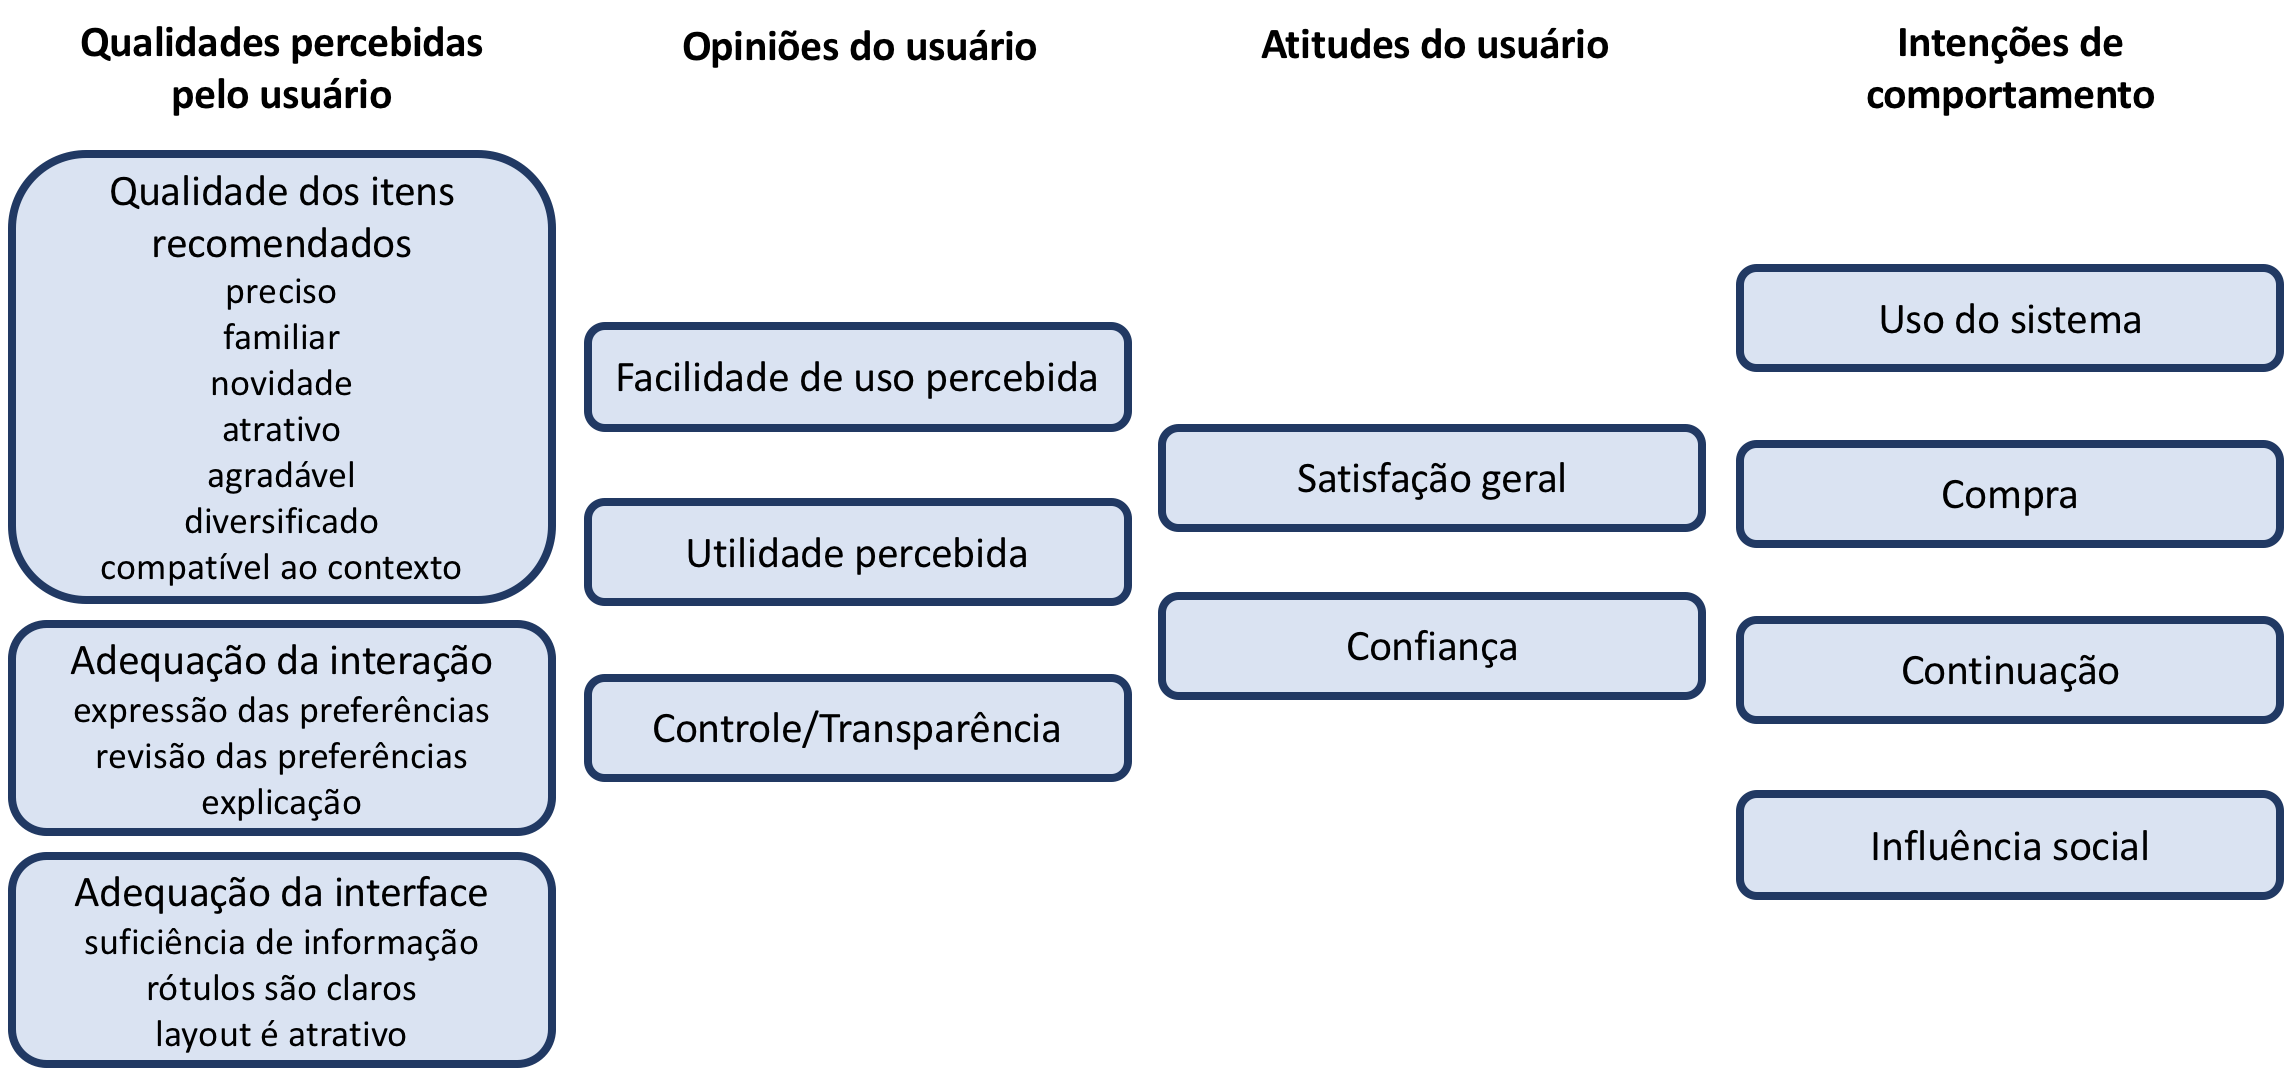
\includegraphics[scale=0.4]{./Figuras/resque-framework-traduzido.png}
  \end{center}
  \legend{Fonte: \citeonline{pu2011user}}
\end{figure}

\section{Considerações sobre o capítulo}

Nesse capítulo foram apresentados os principais conceitos relacionados a Sistemas de Recomendação (SRs) Sensíveis ao Tempo.
Foram apresentadas desde as abordagens tradicionais, passando pelos SR Sensíveis Contexto e os seus paradigmas até as
categorias de SRs Sensíveis ao Tempo definidas em \citeonline{de2017time}.

Dentre as categorias de SRs Sensíveis ao Tempo apresentadas na Seção \ref{section:sr-sensivel-tempo}, a utilizada por esse
trabalho é o \textit{Decay}. Nessa categoria é considerado que o interesse do usuário por um item acessado diminui com o passar
do tempo. Neste sentido, considerando que o acesso a um item é um indicativo do interesse do usuário, os itens acessados
mais recentemente têm um peso maior na identificação dos interesses do usuário, i.e., na definição do perfil do usuário.

Além disso, foram apresentadas as formas de avaliação de um SR como definido por \citeonline{shani2011evaluating}. Neste
trabalho será utilizada uma avaliação pela perspectiva do usuário, como orientado por \citeonline{pu2012evaluating}. Por isso, é
apresentado o \textit{framework} definido por \citeonline{pu2011user} que busca avaliar a experiência do usuário através de um
questionário com 60 questões dividas nos quatro construtos do \textit{framework}. Para ser utilizado, é necessário
selecionar quais das questões serão utilizadas, pois como citado por \citeonline{pu2011user} nem todas as questões se
aplicam a todos os SRs.

\chapter{Trabalhos relacionados}\label{chapter:trabalhos-relacionados}

Todos os trabalhos descritos neste capítulo foram selecionados dentre os artigos analisados no mapeamento sistemático
da literatura \cite{de2017time} sendo considerados aqueles que estão enquadrados dentro da categoria de Decaimento no que
se refere ao uso do tempo no algoritmo de recomendação, independente do domínio de aplicação. No total, sete trabalhos
foram selecionados, sendo apenas um da área educacional.

\section{Fan et al. 2015}

O trabalho de \citeonline{fan2015modeling} realiza a recomendação de \textit{web services}, considerando a avaliação do serviço
através da medição do \textit{Quality of Service} (QoS). QoS considera características do serviço como tempo de resposta,
disponibilidade, taxa de serviço, etc. Os autores consideram que a capacidade de prever a qualidade de um serviço diminui
conforme o tempo que passou da última invocação desse serviço, devido a possíveis encerramentos do serviço, falhas na
rede, etc. Por isso, a recomendação de serviços dos autores combina a similaridade entre os serviços invocados
pelos usuários com uma função de decaimento que considera que a QoS diminui com o passar do tempo em um algoritmo de Filtragem
Colaborativa. O modelo de decaimento proposto considera que as invocações mais recentes de dois usuários a um serviço devem ter um impacto maior no cálculo da similaridade entre os
usuários. A função de decaimento de um item $k$ é definida na Equação \ref{eq:fan-funcao-decaimento}.

\begin{equation}
  \label{eq:fan-funcao-decaimento}
  f(t_{i,k}, t_{j,k}) = e^{-\alpha \left|t_{atual} - \Delta t \right|}
\end{equation}

Onde: $t_{i,k}$ e $t_{j,k}$ são os tempos no qual os usuários $u_i$ e $u_j$ invocaram o serviço $k$; $\alpha$ é o fator
de decaimento; e $\Delta t$ é a variação de tempo combinando o acesso do usuários $u_i$ e $u_j$ e é calculada com a
fórmula apresentada na Equação \ref{eq:fan-fator-decaimento}.

\begin{equation}
  \label{eq:fan-fator-decaimento}
  \Delta t = \frac{(\Delta t_i + \Delta t_j)}{2}
\end{equation}

Onde $\Delta t_i$ é o intervalo de tempo entre a invocação do serviço pelo usuário $u_i$ ao serviço e o tempo atual e
$\Delta t_j$ é o intervalo de tempo entre a invocação do mesmo serviço pelo usuário $u_j$ e o tempo atual. Assim, a
similaridade dos usuários  diminui quanto maior for o $\Delta t$.

A nota do serviço $k$ é considerada como a combinação do QoS com a função de decaimento e é calculada através da Equação \ref{eq:fan-avaliacao}.

\begin{equation}
  \label{eq:fan-avaliacao}
  r_{u_i, s_k, t} = r_{u_i, s_k} \cdot f(t_{i,k}, t_{j,k})
\end{equation}

Onde $r_{u_i, s_k}$ é o QoS do serviço $k$ na sua última invocação e $r_{u_i, s_k, t}$ representa o QoS considerando o decaimento
desde a sua última invocação. Os autores utilizam a nota resultado da função apresentada anteriormente para calcular a similaridade dos itens utilizando
o coeficiente de Pearson. A Equação \ref{eq:fan-similaridade} apresenta o coeficiente de Pearson utilizado pelos autores
que considera a função de decaimento.

\begin{equation}
  \label{eq:fan-similaridade}
  sim(u_1, u_j, t) = \frac{\sum_{s_k \in w_{u_i, u_j}}{(r_{u_i, s_k, t} - \overline{r_{u_i}})(r_{u_j, s_k, t} - \overline{r_{u_j}})}}{\sum_{s_k \in w_{u_i, u_j}}{(r_{u_i, s_k, t} - \overline{r_{u_i}})}^2 \sum_{s_k \in w_{u_i, u_j}}{(r_{u_j, s_k, t} - \overline{r_{u_j}})}^2}
\end{equation}

Onde $\overline{r_{u_i}}$ representa a média do QoS dos serviços invocados pelo usuário $u_i$, $\overline{r_{u_j}}$
representa a média do QoS dos serviços invocados pelo usuários $u_j$ e $w_{u_i, u_j}$ é o conjunto dos itens em comum
invocados pelos usuários $u_i$ e $u_j$. Utilizando essa fórmula de similaridade é possível calcular a similaridade entre
os usuários e encontrar os que são mais similares.

A proposta dos autores considera também a localização desses usuários para calcular a similaridade. Quanto mais próximos
eles estão, mais similares eles são considerados.

Os autores realizaram experimentos com a base de dados WS-Dream comparando o algoritmo proposto com outros 6 algoritmos: Recomendação
considerando todos os usuários (RBA), Filtragem Colaborativa Usuário-Usuário utilizando a Correlação de Pearson (UPCC),
Filtragem Colaborativa Item-Item utilizando a Correlação de Pearson (IPCC), \textit{Context-Aware Service Recommender}
(CASR), Método que considera a preferência do usuário de acordo com a sua localização (CASR-UP) e UPCC que considera o
decaimento (ITRP-WS). A avaliação foi realizada utilizando uma estratégia \textit{offline} e as métricas utilizadas para
a comparação foram MAE e RMSE.

Primeiramente os autores realizaram um experimento verificando a influência dos paramêtros dos algoritmos. Esses parâmetros são
considerados para decidir quais são os itens considerados significantes, ou seja, depois de calculada nota prevista para
os itens, decidir qual o limite mínimo para que um item seja recomendado. O segundo experimento avaliou a influência da
proporção da base de treino e de teste no experimento. E por último, para os algoritmos que utilizavam a Filtragem
Colaborativa foi avaliado a influência da quantidade de k-vizinhos considerada na eficiência do algoritmo. Os resultados
desses experimentos mostraram que o algoritmo proposto foi melhor que os outros 6 algoritmos analisados.

\section{Luo et al. 2010}

O trabalho de \citeonline{luo2010context} propõe um modelo de recomendação sensível ao contexto para ambientes de
aprendizagem pervasivos. Esse modelo utiliza uma abordagem híbrida (baseada em conteúdo com filtragem colaborativa)
com uma personalização pelo contexto. Três tipos de contexto são definidos:

\begin{enumerate}
\item contexto do aluno, que possui as seguintes dimensões: tipo de dispositivo, ambiente (localização), perfil
(informações pessoais, como nome e afiliação), preferências (recursos pelos quais o aluno tem interesse), processo de
aprendizagem (histórico de materiais acessados), pedido de acesso (a recursos educacionais massivos).
\item contexto do serviço, que possui as seguintes dimensões: ambiente (localização), perfil (nome, parâmetros,
retornos), QoS (parâmetros de qualidade do serviço, como carga de trabalho, reputação, disponibilidade, segurança, etc.).
\item contexto do recurso, que segue o \textit{China ELearning Technology Standard} que define as dimensões de um recurso
educacional. Esse padrão define as dimensões como sendo: perfil (informações sobre o recurso, como Título, Assunto,
Palavras-chave), criador (nome, organização), audiência (tipo de educação, nível de ensino).
\end{enumerate}

O modelo de recomendação proposto pode ser dividido em dois passos: \textit{Logic-Based Resource Relevant Degree} e
\textit{Situation-Based Resource Relevant Degree}.

Na etapa do \textit{Logic-based Resource Relevant Degree} é feita uma análise do histórico de recursos acessados pelo aluno e as
suas preferências. Esse passo combina a abordagem baseada em conteúdo, filtragem colaborativa e os padrões sequenciais
de acesso.

A abordagem baseada em conteúdo considera as múltiplas dimensões dos recursos como assunto, assunto secundário, nível
de ensino, etc. Nessa abordagem, é inserido um conceito de \textit{Preference Energy} (PE) para refletir a variação do interesse
do usuário com o passar do tempo. O PE indica que o interesse de um usuário a um item acessado diminui com o passar do
tempo. Os autores definem a diminuição da PE pela fórmula apresentada na Equação \ref{eq:luo-preference-energy}.

\begin{equation}
  \label{eq:luo-preference-energy}
  PE_{attenuation}(x) = e^{- \lambda (x-1)}, com \ x \geqslant 1
\end{equation}

Onde $x$ é a ordem do recurso na lista de acessos do usuário e $\lambda$ é o parâmetro de decaimento. Esse valor do PE,
combinado com as avaliações feitas pelos usuários para os itens, são utilizadas para gerar uma \textit{Individual Preference Tree}
que auxilia o cálculo da similaridade dos recursos candidatos a serem recomendados.

A \textit{Individual Preference Tree} utilizada pela abordagem baseada em conteúdo também é considerada pelo algoritmo de
filtragem colaborativa definida pelos autores para encontrar os k-vizinhos mais similares. Dessa forma, não só usuários
que acessaram os mesmos itens podem ser considerados vizinhos (como na filtragem colaborativa tradicional), mas também
usuários que acessaram itens similares entre si (mesmo assunto, palavras-chave, etc.) e os avaliaram de forma similar.

O último método de recomendação utilizado pela etapa chamada \textit{Logic-based Resource Relevant Degree} utiliza os padrões
sequencias de acesso dos usuários aos recursos. O algoritmo utilizado para a mineração dos padrões sequencias é o
PrefixSpan, que procura sequências (ou subsequências) que apareceram em pelo menos $\mu$ acessos. Baseado na árvore de
padrões sequenciais resultantes do algoritmo de mineração, é calculado quais os itens mais prováveis de serem acessados
de acordo a sequência atual do usuário. A proposta dos autores define que o algoritmo de mineração de sequências deve
ser executado de forma \textit{offline}, para garantir a resposta em um tempo hábil.

A etapa de \textit{Logic-based Resource Relevant Degree} combina o conjunto de recursos recomendados dos três algoritmos
descritos, removendo da lista os recursos já acessados pelo usuário.

Na etapa de \textit{Situation-based Resource Relevant Degree} é considerado que mesmo um recurso que combine com as preferências
do usuário pode não ser adequado para a recomendação se o contexto do usuário (dispositivo, ambiente) não for adequado
para utilizar o recurso. Para isso, no contexto dos recursos são descritos quais os dispositivos nos quais a utilização do
recurso é adequada e no contexto do usuário é descrito qual o dispositivo do usuário. Também é considerado o grau de
satisfação no tempo para acessar um determinado recurso. Isso pode ser calculado pelo tamanho do recurso e a velocidade
de internet do usuário. Combinando essas duas características é possível ter uma recomendação mais adequada a situação
atual do aluno.

O algoritmo de recomendação proposto pelos autores então calcula uma lista de recursos candidatos a recomendação
utilizando os algoritmos de \textit{Logic-Based Resource Relevant Degree} e remove dessa lista os recursos que não satisfaçam o
dispositivo do usuário e a satisfação mínima com o tempo de resposta esperado.

Esse algoritmo foi avaliado através de uma avaliação \textit{offline} utilizando o base de dados do Movielens, onde foram adicionados dados de
contexto às interações existentes na base. As métricas utilizadas para avaliar o algoritmo foram \textit{Precision}, Utilidade e
Validade (razão entre a quantidade de itens apropriados para o tipo de conexão do usuário e o total de itens existentes).
A avaliação foi feita em relação aos seguintes  algoritmos tradicionais de recomendação: Algoritmo Baseado em Conteúdo
utilizando o modelo de espaço vetorial, Filtragem Colaborativa combinando a abordagem Usuário-Usuário com a Item-Item, Abordagem
Híbrida. Em comparação aos algoritmos tradicionais o algoritmo proposto teve melhores resultados no
experimento realizado.

\section{Benčič e Bieliková 2012}

O sistema de recomendação proposto por \citeonline{bencic2012action} busca recomendar ações aos usuários no momento que
for propício, de acordo com o contexto do usuário, e não apenas quando uma ação do interesse do usuário é encontrada.
Uma ação se refere a qualquer coisa que seja utilizada pelo usuário final de uma aplicação.

O método proposto para a recomendação representa o contexto do usuário através de símbolos, onde cada símbolo é
composto de duas partes – onde uma representa a dimensão e a outra representa a situação particular. Por exemplo,
$Clima:Limpo$. Para cada símbolo do contexto do usuário é atribuído um valor no intervalo $(0, 1)$ que indica a convicção
de que o usuário está naquele contexto.

A convicção de que o usuário está em determinado contexto é observada de tempos em tempos. Esse intervalo depende da
velocidade de conexão do dispositivo do usuário, nível da bateria, etc. A convicção do usuário estar em determinado
contexto diminui com o passar o tempo (supondo que uma nova observação demore a acontecer). Por isso, os autores
utilizam uma função de decaimento para essa convicção conforme a Equação \ref{eq:bencic-conviccao}.

\begin{equation}
  \label{eq:bencic-conviccao}
  CF_t = \frac{CF_b}{(1+r)^t}
\end{equation}

Onde $CF_t$ é a convicção calculada em função do tempo $t$, $CF_b$ é a convicção base, $r$ é o fator de decaimento e $t$
é o tempo em horas passado desde a última observação.

As ações são modeladas através de um conjunto de regras. As regras são definidas automaticamente através do feedback do
usuário e são representadas pelos antecedentes (em que situação a regra se aplica) e a consequência (a ação associada
aquela situação). As regras também possuem um decaimento na convicção com o passar o tempo. Porém, nesse caso o
decaimento não é constante, como acontece para o decaimento da convicção do contexto do usuário. Para as regras, o fator
de decaimento é calculado para que a convicção não chegue a zero ao acontecer um longo período sem observações.

Combinando as convicções nas regras criadas com as convicções no contexto do usuário, são encontradas as ações com
maior probabilidade de serem adequadas. O modelo de recomendação considera não apenas a última observação, mas sim uma
combinação das últimas observações e suas respectivas convicções (com o fator de decaimento aplicado).

A avaliação do sistema foi feita realizando simulações de possíveis interações de um usuário imaginário em um ambiente
de recomendação de notícias durante o período de um mês. Nessa simulação, o objetivo foi calcular as recomendações de
notícias para três perfis de usuários: um usuário que lê notícias todos os dias pela manhã; outra que lê notícias apenas
nas segundas pela manhã e sextas a noite; e outro que começa lendo as notícias apenas nas segundas pela manhã e muda o
seu comportamento com o passar do tempo para a leitura as sextas a noite. Os resultados mostraram que o método conseguiu
compreender o comportamento dos três tipos de usuário com uma Precisão e um \textit{Recall} de quase 100\%.

\section{Hawalah e Fasli 2014}

O trabalho de \citeonline{hawalah2014utilizing} propõe um método de recomendação utilizando o contexto do usuário
representado através de ontologias. O algoritmo proposto pode se adequar a diversos domínios, de forma que o contexto
seja incorporado aos interesses do usuário independente do que são os itens que serão recomendados. Além disso, o método
considera não só o contexto atual do usuário, mas também os contextos capturados anteriormente. Os autores separam o
método em três fases: Extração da informação, Aprender o perfil do usuário e Personalização.

A etapa de Extração da informação é realizada por um agente de captura dos dados que é genérico o suficiente para ser
adaptado de acordo com o domínio. Em determinados domínios pode ser utilizado uma coleta perguntando explicitamente os
interesses e o contexto ao usuário, enquanto em outros domínios é mais adequado capturar de forma implícita pela
navegação do usuário.

A informação bruta capturada (seja de forma explícita ou implícita) é processada pelo agente extrator, responsável por
extrair informação de mais alto nível. Esse agente está associado a dois tipos de bases de conhecimento: ontologias e
taxonomias. O agente realiza um mapeamento dos itens que o usuário demonstrou interesse em conceitos da ontologia de
referência, enquanto também extrai dimensões do contexto de mais alto nível utilizando-se das taxonomias de contexto.

A segunda etapa, responsável por compreender o perfil do usuário, utiliza a abordagem de Pré-filtragem Contextual para
definir qual a parte do perfil do usuário é relevante. É utilizada um método de micro-perfis, onde as
informações do perfil do usuário (itens acessados, notas dadas) que aconteceram em contextos similares ao atual são
consideradas mais relevantes para a recomendação. Para isso, é calculado a importância dos conceitos em cada contexto
possível, de acordo com as informações do perfil do usuário. Nesse cálculo, é considerada a frequência com que o
conceito aparece naquele determinado contexto, bem como a frequência com que esse conceito aparece em outros contextos
e a frequência com que outros conceitos aparecem nesse contexto.

Ainda no cálculo da importância do conceito em determinado contexto, é considerado que os interesses do usuário podem
mudar com o tempo. Para isso, é incluído na fórmula o fator de Recência (do inglês \textit{Recency}), de forma que os interesses
demonstrados pelo usuário mais recentemente são considerados mais importantes. A fórmula apresentada na Equação
\ref{eq:hawalah-recencia} apresenta o cálculo da recência.

\begin{equation}
  \label{eq:hawalah-recencia}
  Recency(c_j, ce_l) = \frac{1}{(1+\log(d_t - d_l) \times \alpha)}
\end{equation}

Onde $d_t$ é a data de inicialização do cálculo, $d_l$ é a data da última ocorrência do conceito $c_j$ no contexto
$ce_l$ e $\alpha$ é o fator de decaimento.

Dessa forma, como resultado dessa etapa temos os interesses do usuário em cada contexto e o peso de cada um. Essas
informações são utilizadas para construir ontologias de perfil contextual personalizada (CPOP, do inglês, \textit{Contextual
Personalized Ontology Profile}), sendo uma CPOP para cada contexto.

Na terceira etapa de personalização, a ontologia gerada na etapa anterior é utilizada para inferir outros conceitos que
o usuário pode ter interesse, além dos já presentes do seu perfil. Isso é realizado utilizando a técnica de \textit{Spreading
Activation}, que explora as ontologias buscando encontrar os novos conceitos relacionados ao perfil do usuário.
Utilizando essa técnica, é gerada uma lista de recomendações para cada CPOP, que são combinadas para gerar a lista
final de recomendações para o usuário.

A avaliação do trabalho de \citeonline{hawalah2014utilizing} foi através de um Estudo com Usuários, visando uma
avaliação centrada no usuário como descrito por \citeonline{kelly2009methods}. O objetivo da avaliação é verificar se
a recomendação contextual proposta no trabalho fornece uma recomendação mais eficiente do que os métodos tradicionais.
24 usuários participaram da avaliação, onde eles utilizaram um sistema por 30 dias, numa estratégia
\textit{Between-subjects}, i.e., cada grupo testa apenas uma versão do sistema. No total, 4 versões do sistema foram
testadas: o algoritmo proposto (CAPS), o algoritmo proposto sem o uso do contexto (CAPS-C), um método de recomendação
personalizado tradicional chamado pelos autores de Simple-P e um método de recomendação não personalizado chamado de Non-P.

O resultado da avaliação analisou a nota dada pelos usuários para os itens em uma escala de likert de 1 a 4. Sendo itens
com grau 1 e 2 considerados uma recomendação ruim e os itens com grau 3 e 4 considerados uma boa recomendação. Com isso
foi possível calcular a \textit{Precision at N} (P@N). O algoritmo proposto possui o melhor resultado de P@N entre os
algoritmos testados.

\section{Qiao e Zhang 2012}

O trabalho de \citeonline{qiao2015personalized} propõe um algoritmo de recomendação que considera as informações
contextuais disponíveis em dispositivos móveis, como tempo, localização, tipo do dispositivo, etc. O algoritmo de
recomendação é genérico, ou seja, sem um domínio de aplicação definido.

O objetivo dos autores é combinar a Filtragem Colaborativa com o contexto do usuário, considerando a variação temporal
nos seus interesses. Para tal, são encontrados os k usuários com os interesses similares ao usuário atual,
considerando o contexto do usuário, através de técnicas de clusterização. Após encontrados os k vizinhos, utiliza-se
uma fórmula para a predição das notas para itens ainda não acessados pelo usuário com a incorporação de uma função
temporal, como apresentado na Equação \ref{eq:qiao-predicao}. Os itens com as notas previstas mais altas são
recomendados ao usuário.

\begin{equation}
  \label{eq:qiao-predicao}
  p_{u,i} = \overline{r_u} + \frac{\sum_{v \in U}{sim(u, v)(r_{v,i} - \overline{r_v})f(t_{v,i})}}{\sum_{v \in U}{sim(u, v)f(t_{v,i})}}
\end{equation}

Sendo $p_{u,i}$ a nota prevista do usuário $u$ para o item $i$, $\overline{r_u}$ a média das notas dadas pelos usuário
$u$, $sim(u, v)$ a similaridade entre o usuário $u$ e o seu vizinho $v$, $r_{v,i}$ o grau de interesse do usuário $u$
pelo item $i$, $\overline{r_v}$ é a média das notas dadas pelo usuário $v$ e $t_{v,i}$ é o tempo passado desde que o
usuário $v$ utilizou o item $i$. A função $f(t_{v,i})$ é uma função exponencial de decaimento que representa a diminuição do
interesse do usuário por um determinado item. A função de decaimento é definida na Equação \ref{eq:qiao-funcao-decaimento}.

\begin{equation}
  \label{eq:qiao-funcao-decaimento}
  f(t_{v,i}) = e^{-t_{v,i}}
\end{equation}

A avaliação desse algoritmo foi realizada utilizando a base do MovieLens – 100 K, através da métrica MAE. Quando
comparado a Filtragem Colaborativa tradicional o algoritmo proposto alcançou melhores resultados, ou seja, teve uma taxa de erro menor.

\section{Kushwaha et al. 2016}

O trabalho de \citeonline{kushwaha2016inclusion} propõe uma versão modifica da técnica de \textit{Joint Matrix Factorization}
para uso em um sistema de recomendação de músicas incorporado ao Last.fm. A proposta busca reduzir a esparsidade dos
dados e melhorar a qualidade das recomendações. Para isso, é incorporado informações como descrição dos itens, perfil
do usuário e o seu contexto na matriz das notas dadas pelos Usuários para os Itens comumente utilizada na Filtragem
Colaborativa. Assim, a matriz utilizada pelo algoritmo possui uma maior dimensionalidade e complexidade. A técnica de fatoração de
matrizes é essencial para reduzir a dimensão da matriz utilizada e permitir a extração de informações latentes importantes para a
recomendação.

Além disso, no algoritmo proposto por \citeonline{kushwaha2016inclusion} é considerado uma estratégia de \textit{tag-based
user similarity matrix}, i.e., uma variação da Filtragem Colaborativa que utiliza as tags colocadas pelos usuários nos Artistas
e Músicas como forma de comparar os usuários e encontrar os mais similares. Nessa estratétia é considerada a variação
temporal da informação. Os autores consideram o decaimento da importância das \textit{tags} colocadas pelo usuário nos
itens com o passar do tempo. A fórmula utilizada pelos autores para representar o decaimento foi baseada em
\citeonline{iofciu2009time}, que pode ser vista na Equação \ref{eq:kushwaha-funcao-decaimento}.

\begin{equation}
  \label{eq:kushwaha-funcao-decaimento}
  postScore_i = \lambda^{\Delta Time_i}
\end{equation}

Onde $postScore_i$ é a importância temporal da \textit{tag} $i$, $\lambda$ é o fator de decaimento, que deve ser menor do que 1
e foi utilizado por \citeonline{kushwaha2016inclusion} como 0.9 e $\Delta Time_i$ é o tempo passado desde a interação. Além disso,
é considerada a especificidade da \textit{tag} para a nota final da \textit{tag}. A fórmula da especificidade é definida
na Equação \ref{eq:kushwaha-especificidade}

\begin{equation}
  \label{eq:kushwaha-especificidade}
  tagSpecificity_i = \log(50+tagCount_i)
\end{equation}

Onde $tagSpecificity_i$ é o fator de especificidade da \textit{tag} e $tagCount_i$ representa quanta vezes a \textit{tag} foi adicionada
ao item $i$. A nota final da \textit{tag} é calculada conforme a Equação \ref{eq:kushwaha-nota-final}.

\begin{equation}
  \label{eq:kushwaha-nota-final}
  tagScore_i = \frac{\sum_1^n{postScore}}{tagSpecifity_i}
\end{equation}

A fórmula acima combina a importância temporal da \textit{tag} com a sua especificidade. A nota final da \textit{tag}
é incorporada na matriz latente resultado da fatoração de matrizes para servir como fator de decaimento para a importância
das \textit{tags}, representando a variação nos interesses do usuário.

O algoritmo proposto pelos autores foi avaliado utilizando uma base de dados do próprio Last.fm, combinado com a base de
dados do DBpedia para a captura de informações sobre os artistas, compositores e músicas. A avaliação considerou a
métrica RMSE para as previsões para as notas que o usuário daria para um determinado
item comparada com a nota real. Quando comparado com outros dois algoritmos de recomendação que incorporam
informação social para recomendação (chamados BPMFSR e Sorec), o algoritmo proposto por \citeonline{kushwaha2016inclusion} se saiu melhor em 3
das 6 condições de experimento realizadas.

\section{Wei, Khoury e Fong 2013}

\citeonline{wei2013web} descrevem uma proposta de recomendação que utiliza a Filtragem Colaborativa e que aplica um
decaimento temporal na importância das interações dos usuários. No trabalho, é proposto um serviço para a recomendação
de propagandas em redes sociais, que leva em consideração a confiança entre usuários, a reputação dos usuários e as
relações entre usuários. Os autores afirmam que usuários com uma recomendação gerada com base em usuários conhecidos
pelo usuário atual serão mais bem aceitas, assim como usuários no qual ele confia e nos usuários com alta reputação
(especialistas).

O algoritmo de recomendação considera que a importância da relação entre os usuários diminui gradativamente com o tempo.
Então, um comentário realizado hoje deve ter um peso maior que um comentário realizado há um mês atrás quando for
avaliada a relação entre dois usuários. O decaimento é incluído diretamente na fórmula utilizada para realizar a
comparação de similaridade entre dois itens, como pode ser visto a seguir na Equação \ref{eq:wei-similaridade}.

\begin{equation}
  \label{eq:wei-similaridade}
  s_{i,j}(t) = \frac{\sum_{u \in U_i^t \cap U_j^t}{(f_{ui}^\alpha(t) \cdot r_{ui})(f_{uj}^\alpha(t) \cdot r_{uj})}}{\sqrt{\sum_{u \in U_i^t}{(f_{ui}^\alpha(t) \cdot r_{ui})}^2 \sum_{u \in U_j^t}{(f_{uj}^\alpha(t) \cdot r_{uj})}^2}}
\end{equation}

Onde $s_{i,j}(t)$ é a similaridade entre os itens $i$ e $j$, $U_i^t$ é o conjunto de usuários que avaliaram o item $i$ no
tempo $t$, $U_j^t$ é o conjunto de usuários que avaliaram o item $j$ no tempo $t$, a função $f_{ui}^\alpha$ é definida
pelos autores como relevância temporal do item e pode ser vista na Equação \ref{eq:wei-relevancia-temporal} e $r_{ui}$ e
$r_{uj}$ são as avaliações do usuário $u$ para os itens $i$ e $j$.


\begin{equation}
  \label{eq:wei-relevancia-temporal}
  f_{uj}^\alpha(t) = e^{- \alpha (t - t_{ui})}
\end{equation}

Onde fator $\alpha$ é responsável por controlar a taxa de decaimento, $t$ representa o tempo atual e $t_{ui}$ representa
o tempo no qual o usuário $u$ utilizou o item $i$.

Além do decaimento na relevância das relações entre os usuários, os autores também incluem a confiança entre os
usuários e a reputação de especialistas da área na fórmula de similaridade visando melhorar a qualidade das
recomendações.

O algoritmo proposto foi avaliado utilizando três bases de dados: MovieLens, Facebook e Delicious. O algoritmo foi
comparado a outros dois algoritmos: Filtragem Colaborativa usando correlação de Pearson e usando correlação de Pearson
com efeito temporal. As métricas utilizadas foram \textit{Mean Absolute Error} e \textit{Root Mean Square Deviation}.
Os resultados mostraram que o algoritmo proposto melhorou significativamente a qualidade das recomendações.

\section{Considerações sobre o capítulo}

Nesse capítulo foram apresentados sete trabalhos relacionados que utilizam Sistemas de Recomendação (SRs) com o uso do
Decaimento. A tabela \ref{tab:comparacao-trabalhos-relacionados} apresenta um resumo dos trabalhos apresentados e uma comparação com
a proposta desse trabalho.

\begin{table}[hp]
\footnotesize
\caption[Comparação dos trabalhos relacionados]{Comparação dos trabalhos relacionados.}
\label{tab:comparacao-trabalhos-relacionados}
\centering
\begin{tabular}{|p{2cm}|p{2cm}|p{1.9cm}|p{1.6cm}|p{1.5cm}|p{1.7cm}|p{2.2cm}|}
  \hline
  \textbf{Trabalho} & \textbf{Domínio} & \textbf{Abordagem} & \textbf{Constante de decaimento} & \textbf{Tempo absoluto} & \textbf{Avaliação} & \textbf{Algoritmos comparados} \\
  \hline
  \citeonline{fan2015modeling} & \textit{Web Services} & Filtragem Colaborativa & Sim & Sim & Offline, com a base WS-Dream & RBA, UPCC, IPCC, CASR, CASR-UP e ITRP-WS \\
  \hline
  \citeonline{luo2010context} & AVA & Híbrida & Sim & Não & Offline, com a base do Movielens & Abordagens tradicionais: Baseada em Conteúdo, Filtragem Colaborativa e Híbrida \\
  \hline
  \citeonline{bencic2012action} & Genérico & Baseada em Conhecimento & Sim & Sim & Simulações & Nenhum \\
  \hline
  \citeonline{hawalah2014utilizing} & Genérico & Baseada em Conhecimento & Sim & Sim & Estudos com usuários, com 24 usuários durante 30 dias & CAPS-C, Simple-P e Non-P \\
  \hline
  \citeonline{qiao2015personalized} & Genérico & Filtragem Colaborativa & Não & Sim & Offline, com a base do Movielens & Filtragem Colaborativa tradicional \\
  \hline
  \citeonline{kushwaha2016inclusion} & Músicas & Híbrida & Sim & Sim & Offline, com a base da Last.fm & BPMFSR e Sorec \\
  \hline
  \citeonline{wei2013web} & Propagandas & Filtragem Colaborativa & Sim & Sim & Offline, com as bases do Movielens, Facebook e Delicious & Filtragem Colaborativa usando correlação de Pearson com e sem efeito temporal \\
  \hline
  Proposta & AVA & Baseada em Conteúdo & Não & Não & Estudos com usuários, com pelo menos 60 usuários durante 45 dias & Abordagem Baseada em Conteúdo tradicional \\
  \hline
\end{tabular}
\legend{Fonte: O autor.}
\end{table}

Pode-se observar que dos trabalhos relacionados, apenas um é da área educacional, enquanto os outros são aplicados em outros
domínios de aplicação. Além disso, nenhum dos trabalhos apresentados utiliza a abordagem Baseada em Conteúdo. A
abordagem mais comumente utilizada nos trabalhos relacionados é a Filtragem Colaborativa, aparecendo sozinha em três trabalhos
e em mais dois outros trabalhos combinada com outras abordagens (i.e., Abordagem Híbrida).

Dos trabalhos relacionados, apenas um não considera uma Constante de decaimento. Essa Constante de decaimento geralmente
é um valor entre $0$ e $1$ que define a velocidade com que o peso das interações do usuário diminui. Esse valor é definido
pelos autores de forma empírica, não havendo um método para a definição dessa constante. No trabalho de \citeonline{qiao2015personalized},
que não utiliza uma Constante de decaimento, é utilizada um função exponencial para o decaimento do interesse do usuário. Na
proposta do presente trabalho também não utiliza uma Constante de decaimento, pois é um fator que ainda requer estudos para
verificar qual o valor e ideal e esse não é o objetivo desse trabalho. Na proposta deste trabalho é utilizada uma função de decaimento linear,
por ser a função mais simples que poderia ser utilizada.

Também é possível observar que apenas um trabalho não utiliza o Tempo absoluto na função de decaimento. Isso significa que
a maioria dos trabalhos relacionados considera o tempo passado (e.g., em segundos, minutos, horas, etc.) desde a interação
para calcular a importância desta. O trabalho de \citeonline{luo2010context} considera a sequência de itens acessados, dando
uma maior importância para os itens mais recentes de acordo com a posição do item na lista ordenada pelo tempo de acesso.
A proposta desse trabalho utiliza uma estratégia similar a de \citeonline{luo2010context} nesse aspecto.

Sobre a avaliação, pode-se observar que a maioria utiliza uma avaliação \textit{Offline}. \citeonline{bencic2012action} realiza
uma simulação para demonstrar o algoritmo de recomendação, que não se encaixa em nenhuma das formas de avaliação
previstas por \citeonline{shani2011evaluating}. O trabalho de \citeonline{luo2010context}, que é da área educacional assim como a
proposta desse trabalho, utiliza uma avaliação \textit{offline} com a base do Movielens\footnote{Base de dados com
notas dadas por usuários a filmes. Disponível em: https://grouplens.org/datasets/movielens/.}.
Com essa avaliação, apesar de ser realizada de forma correta e apresentar bons resultados, não é possível afirmar que o
SR desenvolvido por \citeonline{luo2010context} teria um bom resultado em um ambiente educacional, porque os dados utilizados
não são da área educacional. No presente trabalho foi realizada uma avaliação com participação de usuários em um ambiente educacional durante uma situação real de uso.

Na avaliação realizada no presente trabalho, o objetivo é comparar o algoritmo proposto com a abordagem Baseada
em Conteúdo tradicional. É possível observar pelos trabalhos relacionados que comparar a proposta com os algoritmos mais
tradicionais da área é algo comumente realizado \cite{fan2015modeling, luo2010context, hawalah2014utilizing, qiao2015personalized, wei2013web}.


\chapter{SR Sensível ao Tempo}\label{chapter:proposta}

Neste capítulo é apresentado o SR Sensível ao Tempo para ambientes educacionais proposto nesse trabalho. O algoritmo proposto
considera o decaimento nos interesses do usuário com o passar do tempo (categoria do \textit{Decay} - Seção \ref{section:decay}). Além
do algoritmo proposto, são apresentados cenários que ilustram o uso desse algoritmo e discussões sobre as suas vantagens.

\section{Algoritmo Proposto}\label{section:algoritmo-proposto}

O algoritmo de recomendação proposto nesse trabalho combina a Abordagem Baseada em Conteúdo com o uso do
contexto temporal através da categoria \textit{Decay} (ver seção \ref{section:decay}). Para o SR, o perfil do usuário é composto pelos
itens acessados por ele. A cada item acessado pelo usuário, são armazenadas as palavra-chaves
do item juntamente com o timestamp do acesso e a sequência desse item no histórico do usuário, começando em $1$ para o
primeiro item acessado. Os itens que serão recomendados também são representados no algoritmo de recomendação por um conjunto de palavras-chave. O cálculo da
relevância de um determinado item $i$ para um usuário $u$ no algoritmo proposto está representado na Equação \ref{eq:relevancia-proposta}.

\begin{equation}
  F(u,i) = S(u,i) \cdot R(I_{u,i}) + A(i)
  \label{eq:relevancia-proposta}
\end{equation}

Onde: $F$ é a função que calcula a relevância de um item $i$ para um usuário $u$; $S$ é a função de similaridade entre
o perfil do usuário $u$ (representado através de conjunto de palavras-chave dos itens acessados) e o item $i$
(representado pelo conjunto de palavras-chave que o caracterizam); $R$ é o maior valor de recência dos itens do conjunto
$I_{u,i}$ (itens acessados pelo usuário $u$ e com alguma similaridade com o item $i$); $A$ é uma função que retorna $1$
se o item $i$ nunca foi acessado pelo usuário $u$ e $0$ se o item já foi acessado.

A função $S$ de similaridade entre o usuário $u$ e o item $i$ pode ser calculada utilizando funções de similaridade como
o Cosseno (ver Seção \ref{subsection:baseada-em-conteudo}). A função de recência $R$, responsável pelo \textit{Decay}, está definida na Equação
\ref{eq:recencia-proposta}.

\begin{equation}
  R(I_{u,i}) = \max_{\{j \in I_{u,i}\}}{\frac{x_j}{\left| I_u \right|}}
  \label{eq:recencia-proposta}
\end{equation}

Onde: $x_j$ é a posição do item $j$ na lista de itens acessados pelo usuário $u$ ordenada de forma crescente pelo
\textit{timestamp} do acesso; e $\left| I_u \right|$ é a quantidade de itens acessados pelo usuário $u$. Essa fórmula considera
que mais de um item acessado pelo usuário pode ser similar ao item $i$, por isso a fórmula retorna a maior recência de
todos os itens presentes no perfil do usuário que são similares a $i$. A seguir temos um exemplo do uso da fórmula da
recência considerando apenas um item, que pode ser estendida para o uso com vários itens e aplicada a função $max$ como descrito na
fórmula acima.

Considerando um usuário $u$ que acessou três itens diferentes nos seguintes \textit{timestamps} (em \textit{epoch}):
Item A acessado em $1503670382$; Item B acessado em $1500027182$; Item C acessado em $1508051582$. A posição desses itens
no histórico do usuário $u$ é: Item A - posição 2, Item B - posição 1 e Item C - posição 3. As equações \ref{eq:recencia-item-a},
\ref{eq:recencia-item-b} e \ref{eq:recencia-item-c} apresentam o resultado do cálculo de recência para cada um dos itens:

\begin{equation}
  R(A) = \max{\frac{2}{3}} = 0.\overline{6}
  \label{eq:recencia-item-a}
\end{equation}

\begin{equation}
  R(B) = \max{\frac{1}{3}} = 0.\overline{3}
  \label{eq:recencia-item-b}
\end{equation}

\begin{equation}
  R(C) = \max{\frac{3}{3}} = 1.0
  \label{eq:recencia-item-c}
\end{equation}

No Algoritmo \ref{alg:proposta-pseudocodigo} é possível observar o pseudocódigo do algoritmo proposto. Nesse algoritmo
estão representadas em mais alto nível as etapas da recomendação. Primeiramente, são buscados no banco de dados os itens acessados
pelo usuário e os itens candidatos a recomendação. Os itens candidatos a recomendação podem ser todos os itens disponíveis
no ambiente ou um subconjunto de itens, de acordo com a necessidade da aplicação.

O cálculo da recência para cada item do perfil do usuário é feito também na fase de inicialização, pois esse cálculo só
precisa ser realizado uma vez. Depois disso, para cada item candidato a ser recomendado para o usuário, é calculada a
similaridade do perfil do usuário (composto pelas palavras-chave dos itens acessados por ele) com as palavras-chave do item
candidato. Além disso, é buscada a lista de itens acessados pelo usuário que são similares ao item candidato. Nessa etapa, também é
encontrado o Item Acessado pelo usuário mais recente que é similar ao item candidato, para utilizar o seu valor de recência no cálculo da Relevância.

\begin{algorithm}
  \caption{Pseudocódigo do Algoritmo de Recomendação Proposto. \label{alg:proposta-pseudocodigo}}

  \SetKwInOut{Input}{input}
  \SetKwInOut{Output}{output}
  \SetKwProg{algoritmoRecomendacaoDecay}{algoritmoRecomendacaoDecay}{}{}

  \algoritmoRecomendacaoDecay{$(Usuário)$}{
    \Input{Usuário que irá receber a recomendação.}
    \Output{Lista com cinco itens recomendados para o usuário.}
    \tcc{Inicialização}
    itens = buscarItensCandidatos()\;
    itensAcessados = buscarItensAcessados(Usuário)\;
    recênciaItensAcessados = calcularRecência(itensAcessados)\;
    relevâncias = \{\}\;
    \tcc{Computação das recomendações}
    \ForEach{$item \in itens$}{
      similaridade = calcularSimilaridade(itensAcessados, item)\;
      itensSimilares = buscarItensSimilares(itensAcessados, item)\;
      recência = calcularMaxRecência(itensSimilares, recênciaItensAcessados)\;
      relevâncias[item] = similaridade * recência + itensAcessados.inclui?(item)\;
    }

    \Return relevâncias.max(5)\;
  }
\end{algorithm}

O cálculo da Relevância para o item candidato é realizado utilizando a Equação \ref{eq:relevancia-proposta}. Os cinco
itens com a maior Relevância são retornados pelo algoritmo para serem recomendados ao usuário.

No Algoritmo \ref{alg:calcular-recencia-pseudocodigo} é demonstrado o cálculo da recência para cada um dos itens do perfil do
usuário, que é utilizado pelo Algoritmo \ref{alg:proposta-pseudocodigo} descrito anteriormente. Para esse cálculo, o próprio registro
de item acessado pelo usuário possui a informação da posição em que se encontra no histórico do usuário e é aplicada
uma versão simplificada da Equação \ref{eq:recencia-proposta}. A função $max$ presente na Equação \ref{eq:recencia-proposta}
não é aplicada nesse momento, sendo calculada apenas a recência
para cada item individualmente. No método descrito no Algoritmo \ref{alg:max-recencia-pseudocodigo} é que a função $max$ será
aplicada para encontrar a maior recência entre os itens similares ao item candidato à recomendação. O algoritmo tem um processo
que difere da Equação \ref{eq:recencia-proposta} justamente para que recência não seja recalculada várias vezes e assim
melhore o seu tempo de processamento.

\begin{algorithm}
  \caption{Pseudocódigo do cálculo da recência para cada item presente no perfil do usuário. \label{alg:calcular-recencia-pseudocodigo}}

  \SetKwInOut{Input}{input}
  \SetKwInOut{Output}{output}
  \SetKwProg{calcularRecencia}{calcularRecência}{}{}

  \calcularRecencia{$(itensAcessados)$}{
    \Input{Lista de registros de acesso do usuário.}
    \Output{Vetor Associativo onde as chaves são os itens acessados pelo usuário e os valores são as recências calculadas para esses itens.}
    recênciaItensAcessados = \{\}\;
    quantidadeItensAcessados = itensAcessados.tamanho()\;

    \ForEach{$itemAcessado \in itensAcessados$}{
      recênciaItensAcessados[item] = itemAcessado.posição() / quantidadeItensAcessados\;
    }

    \Return recênciaItensAcessados\;
  }
\end{algorithm}

\begin{algorithm}
  \caption{Pseudocódigo do cálculo da recência máxima entre os itens do perfil do usuário similares ao item candidato. \label{alg:max-recencia-pseudocodigo}}

  \SetKwInOut{Input}{input}
  \SetKwInOut{Output}{output}
  \SetKwProg{calcularMaxRecencia}{calcularMaxRecência}{}{}

  \calcularMaxRecencia{$(itensSimilares, recênciaItensAcessados)$}{
    \Input{Lista de itens similares ao item candidato a recomendação e vetor associativo com a recência calculada para cada item do perfil do usuário.}
    \Output{Valor máximo de recência entre itens similares.}

    recênciaItensSimilares = recênciaItensAcessados.find(itensSimilares)\;

    \Return recênciaItensSimilares.max(1)\;
  }
\end{algorithm}


\section{Cenário de Uso}

Um cenário de uso do \textit{Decay} é apresentado a seguir. \textit{O aluno Pedro está matriculado em uma disciplina de Estrutura de Dados
que possui quatro tópicos, sendo eles Pilhas, Filas, Listas e Árvores. Nessa disciplina, para cada um dos conteúdos é
aplicada uma prova para avaliar os conhecimentos dos alunos. Para cada conteúdo da disciplina, existem 20 materiais que pode
se acessado normalmente pelo aluno e mais 10 materiais relacionados que só podem ser acessados quando recomendados.
Cada um desses itens é representado pela palavra-chave do conceito em que está relacionado. Até o momento da primeira prova sobre o conteúdo de Pilhas,
Pedro acessou apenas materiais relacionados a Pilhas. O algoritmo de recomendação utilizando a abordagem Baseada em
Conteúdo recomenda para Pedro apenas materiais relacionados a Pilhas. Após a primeira prova, Pedro começa a acessar
materiais relacionados a Filas, o segundo tópico da disciplina. Em uma abordagem Baseada em Conteúdo tradicional as
recomendações continuariam sendo sobre o conteúdo de Pilhas por um bom tempo, pois o perfil de Pedro seria em grande
parte composto por materiais acessados sobre esse assunto. Porém, com o uso do \textbf{Decay}, no momento em que Pedro começar a
acessar materiais sobre Filas o algoritmo de recomendação dará um peso maior para esses materiais (sem ignorar os itens
acessados anteriormente) e em pouco tempo Pedro já estará recebendo recomendações sobre o novo tópico estudado. Da mesma
forma, se Pedro voltar a acessar conteúdos anteriores para relembrar algum conceito, o SR também perceberá isso e
recomendará itens relacionados ao primeiro conteúdo novamente.}

Agora será apresentado em mais detalhe qual seria o comportamento do algoritmo proposto nesse cenário de uso apresentado.
Ao estudar o primeiro assunto da disciplina, Pedro acessa os conteúdos relacionados a Pilhas e no seu perfil
o SR formará o seu perfil com vários itens representados pela palavras-chave ''Pilha''. O SR, ao gerar uma recomendação,
irá encontrar um valor de similaridade alto entre o perfil do usuário e os itens candidatos a recomendação que também possuam
a palavra-chave ''Pilha''. Como todos os itens do perfil do usuário nesse momento tem a palavra-chave ''Pilha'', a recência não
terá um impacto importante nesse momento, pois independente do item que for mais recente a recomendação será a mesma. Na
Tabela \ref{tab:cenario-de-uso-1} é possível observar de forma resumida o comportamento do algoritmo (estamos considerando
que nenhum item recomendado tenha sido acessado).

\begin{table}[h]
\footnotesize
\caption[Cenário de Uso: comportamento do algoritmo após o acesso de itens relacionados a pilhas.]{Cenário de Uso: comportamento do algoritmo após o acesso de itens relacionados a pilhas.}
\label{tab:cenario-de-uso-1}
\centering
\begin{tabular}{|p{2cm}|p{2.5cm}|p{2.5cm}|p{2.5cm}|p{2.5cm}|}
  \hline
  \textbf{Retornos} & \textbf{Itens relacionados a pilhas} & \textbf{Itens relacionados a filas} & \textbf{Itens relacionados a listas} & \textbf{Itens relacionados a árvores} \\
  \hline
  Similaridade & $1.0$ & $0.0$ & $0.0$ & $0.0$ \\
  \hline
  Recência & $1.0$ & $0.0$ & $0.0$ & $0.0$ \\
  \hline
  Acessado ou não & $1.0$ & $1.0$ & $1.0$ & $1.0$ \\
  \hline
  Relevância & $2.0$ & $1.0$ & $1.0$ & $1.0$ \\
  \hline
\end{tabular}
\legend{Fonte: O autor.}
\end{table}

Dessa forma, como é possível ver na Tabela \ref{tab:cenario-de-uso-1} os itens relacionados a pilhas terão uma maior Relevância e serão os itens recomendados.
A partir do momento que o usuário comece a acessar itens relacionados a filas, o algoritmo passará a dar uma importância
maior a itens relacionados a esse segundo tópico. Na Tabela \ref{tab:cenario-de-uso-2} é possível observar o
comportamento do algoritmo nesse caso.

\begin{table}[h]
\footnotesize
\caption[Cenário de Uso: comportamento do algoritmo após o acesso de itens relacionados a filas.]{Cenário de Uso: comportamento do algoritmo após o acesso de itens relacionados a filas.}
\label{tab:cenario-de-uso-2}
\centering
\begin{tabular}{|p{2cm}|p{2.5cm}|p{2.5cm}|p{2.5cm}|p{2.5cm}|}
  \hline
  \textbf{Retornos} & \textbf{Itens relacionados a pilhas} & \textbf{Itens relacionados a filas} & \textbf{Itens relacionados a listas} & \textbf{Itens relacionados a árvores} \\
  \hline
  Similaridade & $0.7$ & $0.3$ & $0.0$ & $0.0$ \\
  \hline
  Recência & $0.35$ & $1.0$ & $0.0$ & $0.0$ \\
  \hline
  Acessado ou não & $1.0$ & $1.0$ & $1.0$ & $1.0$ \\
  \hline
  Relevância & $1.245$ & $1.3$ & $1.0$ & $1.0$ \\
  \hline
\end{tabular}
\legend{Fonte: O autor.}
\end{table}

É possível observar na Tabela \ref{tab:cenario-de-uso-2} que, mesmo o perfil do usuário sendo ainda mais similar a itens com a palavra-chave ''Pilha'',
o impacto da Recência no algoritmo fez com a Relevância dos itens relacionados a filas seja maior e, dessa forma, esses
itens sejam recomendados. Supondo que o aluno Pedro decida voltar a acessar itens relacionados a pilhas para
recapitular os conteúdos. O comportamento do algoritmo nesse caso é apresentado na Tabela \ref{tab:cenario-de-uso-3}.

\begin{table}[h]
\footnotesize
\caption[Cenário de Uso: comportamento do algoritmo após o aluno voltar a acessar itens relacionados a pilhas.]{Cenário de Uso: comportamento do algoritmo após o aluno voltar a acessar itens relacionados a pilhas.}
\label{tab:cenario-de-uso-3}
\centering
\begin{tabular}{|p{2cm}|p{2.5cm}|p{2.5cm}|p{2.5cm}|p{2.5cm}|}
  \hline
  \textbf{Retornos} & \textbf{Itens relacionados a pilhas} & \textbf{Itens relacionados a filas} & \textbf{Itens relacionados a listas} & \textbf{Itens relacionados a árvores} \\
  \hline
  Similaridade & $0.75$ & $0.25$ & $0.0$ & $0.0$ \\
  \hline
  Recência & $1.0$ & $0.7$ & $0.0$ & $0.0$ \\
  \hline
  Acessado ou não & $1.0$ & $1.0$ & $1.0$ & $1.0$ \\
  \hline
  Relevância & $1.75$ & $1.175$ & $1.0$ & $1.0$ \\
  \hline
\end{tabular}
\legend{Fonte: O autor.}
\end{table}

Como pode ser observado na Tabela \ref{tab:cenario-de-uso-3}, algoritmo percebe que o aluno voltou a um tópico já estudado anteriormente e
voltaria a recomendar itens relacionados a isso. Como o perfil do aluno é composto ainda por muitos itens relacionados ao tópico
de Pilhas acessado primeiramente, ao voltar a acessar esses itens o algoritmo voltará a recomendar esses itens
ao aluno.

\section{Discussão Sobre o Algoritmo Proposto}

Um ponto negativo da Filtragem Colaborativa é a necessidade de uma comunidade de usuários ativa, que nem sempre é
possível em um AVA onde as turmas muitas vezes são menores (entre 10 e 100 alunos). A Abordagem Baseada
em Conteúdo é considerada para o SR proposto porque essa abordagem permite a recomendação em um sistema que não possui uma
comunidade ativa e pode suprir as necessidades desse domínio.

Os SRs Sensíveis ao Tempo tem uma vantagem em relação à outros SRs Sensíveis ao Contexto por a informação temporal ser
mais simples de capturar e manipular que outras informações contextuais, e.g., localização. Além disso, esses tipos de
algoritmos estão sendo explorados em outros domínios de aplicação, como pode ser visto nos 88 artigos analisados no
Mapeamento Sistemático realizado \cite{de2017time}, e demonstraram bons resultados. Por isso, esse trabalho busca
aplicar o contexto temporal no algoritmo de recomendação na área educacional (na qual foram encontrados apenas quatro
trabalhos) e avaliar os resultados.

A escolha do \textit{Decay} se justifica como forma de procurar minimizar uma das grandes desvantagens da abordagem Baseada em Conteúdo: a
Superespecialização. Na abordagem Baseada em Conteúdo as recomendações seriam geradas levando em conta todos os itens
acessados pelo usuário igualitariamente. Enquanto ao aplicar o \textit{Decay}, os itens acessados mais recentemente possuem um
grau de importância maior para o algoritmo do que itens acessados anteriormente. Dessa forma, mesmo que o usuário
tenha acessado muitos materiais sobre determinado assunto, ao começar a acessar materiais sobre outro assunto o algoritmo de
recomendação consegue rapidamente se adaptar e gerar recomendações sobre esse novo conteúdo.

O algoritmo proposto nesse trabalho considera o decaimento no peso dos itens do perfil do usuário em função da posição
do item na sequência de materiais acessados, como mostrado na Seção \ref{section:algoritmo-proposto}, e não na quantidade de tempo passada em
segundos como feito na maioria dos trabalhos relacionados mostrados no Capítulo \ref{chapter:trabalhos-relacionados}. Isso é uma vantagem, pois no domínio
educacional o passar do tempo não é tão relevante quanto em outros domínios, como na recomendação de \textit{Web Services} por
exemplo.

Os alunos em um AVA podem ter ritmos de estudo diferentes e, por isso, é assumido nesse trabalho que faz
mais sentido analisar quantos itens foram acessados desde do acesso de determinado material do que o tempo passado desde
a interação. Dessa forma, esse algoritmo não considera se o usuário acessou todos os itens do seu perfil em um
único dia, ou se ele acessou metade do materiais na primeira semana do curso e a outra metade na última semana ou se ele
acessou alguns materiais todos os dias durante o curso.

Além disso, no algoritmo proposto nesse trabalho não é definido um fator de decaimento único para os todos os usuários como nos trabalhos
relacionados apresentados no Capítulo \ref{chapter:trabalhos-relacionados}. Isto porque é necessário considerar
que cada aluno tem um estilo de aprendizagem diferente e o decaimento para um aluno poderia ser diferente do decaimento
para outros alunos. E não foram encontrados nos trabalhos relacionados que mostrem um modelo para calcular o fator de decaimento de forma
personalizada para cada usuário. Em geral, os autores utilizam o fator de decaimento escolhido de forma empírica e
aplicam o mesmo fator para todos os usuários.

\section{Considerações sobre o capítulo}

Nesse capítulo é apresentada a proposta desse trabalho. O algoritmo proposto utiliza a abordagem Baseada em Conteúdo em
conjunto com o uso do tempo através da categoria \textit{Decay}, ou seja, é dado um peso menor na recomendação para os
itens acessados a mais tempo pelo usuário e um peso maior para os itens mais recentes. No Sistema de Recomendação (SR)
proposto é combinada a similaridade entre o perfil do usuário e os itens, a recência dos itens acessados pelo usuário e
se os links recomendados já foram ou não acessados. O algoritmo proposto será avaliado utilizando o experimento descrito
no Capítulo \ref{chapter:experimento}.



\chapter{Experimento}\label{chapter:experimento}

Neste capítulo é apresentado o experimento que realizado para a avaliação da proposta apresentada no Capítulo \ref{chapter:proposta}.
Para avaliar a proposta deste trabalho foi utilizada uma avaliação pela perspectiva do usuário, que segundo a definição de
\citeonline{shani2011evaluating} se encaixa em um Estudo com usuários. O algoritmo proposto será incorporado ao ambiente
\adaptweb e avaliado em uma situação real de uso em um Minicurso de Algoritmos desenvolvido por \citeonline{santos2017addie}.
Na Seção \ref{section:planejamento-experimento} é descrito o ambiente \adaptweb no qual a proposta será incorporada,
as mudanças realizadas no ambiente para o experimento, o objetivo do experimento e o teste piloto realizado. A Seção
\ref{section:execucao-experimento} descreve o experimento que foi realizado e Seção \ref{section:analise-experimento} apresenta
as análises estatísticas realizadas no questionário de satisfação e no uso do Sistema de Recomendação (SR).

\section{Planejamento}\label{section:planejamento-experimento}

\subsection{Descrição do Ambiente \adaptweb}

O \adaptweb (Ambiente de Ensino-Aprendizagem Adaptativo na Web) é um sistema open source
que consiste em um AVA capaz de adaptar o conteúdo, a apresentação e a navegação em determinado curso às características
e preferências do aluno \cite{gasparini2009adaptweb}. A Subseção \ref{subsection:estrutura-adaptweb} apresenta a Estrutura Geral do
\adaptweb.

\subsubsection{Estrutura do \adaptweb}\label{subsection:estrutura-adaptweb}

A estrutura do \adaptweb é composta por quatro módulos: (1) o módulo de autoria; (2) o
módulo de armazenamento em XML (Extensible Markup Language); (3) o módulo de adaptação do conteúdo baseado no modelo do
usuário e (4) o módulo de interface adaptativa \cite{gasparini2003interface}, conforme pode ser visto na Figura
\ref{fig:adaptweb-arquitetura}.

\begin{figure}[htb]
  \caption{\label{fig:adaptweb-arquitetura}Estrutura do \adaptweb}
  \begin{center}
      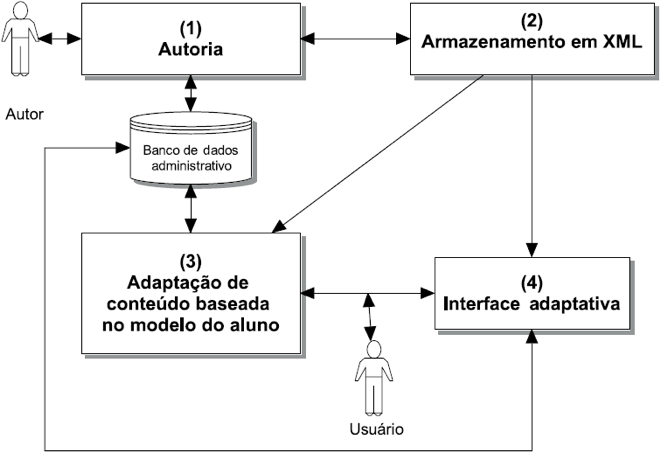
\includegraphics[scale=1.0]{./Figuras/adaptweb-arquitetura.png}
  \end{center}
  \legend{Fonte: \citeonline{gasparini2003interface}}
\end{figure}

O módulo de autoria (1) consiste na organização do conteúdo instrucional a ser disponibilizado para o aluno, sendo que
este conteúdo pode ter arquivos classificados como conceito, exemplos, exercícios e materiais complementares
\cite{gasparini2003interface}. Ao criar um conteúdo no sistema, o autor pode definir para quais cursos e disciplinas
deseja que o conteúdo ou arquivo esteja disponível. Isto significa que um aluno de um Curso X e de outro Curso Y,
matriculados em uma mesma disciplina, podem ter conteúdos distintos, conforme definido pelo professor. Por exemplo, a
disciplina de Cálculo I pode ser oferecida para os cursos de Ciência da Computação e Engenharia Elétrica e sua
abrangência e profundidade pode ser distinta para cada curso.

Em \citeonline{de2015sistema}, foi proposto uma nova categoria para os conteúdos chamada Links de Apoio. Esses Links de Apoio
são links externos ao ambiente \adaptweb que são cadastrados pelo professor como um
material alternativo de estudo e não estão diretamente atrelados á nenhum conceito em específico. O objetivo foi criar
uma nova categoria de materiais que poderia ser recomendada para o usuário a qualquer momento de sua interação.

O módulo de armazenamento em XML (2) é responsável por organizar os conteúdos e arquivos disponibilizados pelo autor em
um arquivo XML \cite{gasparini2003interface}. É utilizada a representação através de XML devido à sua alta
flexibilidade, oferecendo a estruturação dos documentos de forma independente da apresentação.

O módulo de adaptação do conteúdo baseado no modelo do aluno (3) é responsável por adaptar o conteúdo da disciplina
para cada curso. Por fim, o módulo de interface adaptativa (4) é responsável pela adaptação da navegação e da
apresentação da interface do ambiente de acordo com o curso, preferências do modo de navegação (modo tutorial ou livre)
e o conhecimento do usuário \cite{gasparini2003interface}.

\subsubsection{Sistema de Recomendação no \adaptweb}

Na Subseção \ref{subsection:estrutura-adaptweb} foi apresentada a estrutura do ambiente \adaptweb, que possui quatro categorias
de materiais para cada conteúdo. Além disso, existe uma outra categoria chamada Links de Apoio com o propósito de ser um
material auxiliar e que pode ser recomendado a qualquer momento para o usuário.

Fazendo uma relação da estrutura do \adaptweb com o algoritmo proposto no Capítulo \ref{chapter:proposta}, os itens de
das categorias Conceito, Materiais Complementares e os próprios Links de Apoio serão considerados para a composição do perfil do usuário. Todos os
materiais acessados em cada uma das categorias é representado através das palavras-chave, e
essas palavras-chave farão parte do perfil do aluno a partir do momento em que este acessar o material. Já para os itens
recomendados, apenas os Links de Apoio serão utilizados.

Como no ambiente \adaptweb as palavras-chave para o itens podem ser cadastradas pelo professor da disciplina, não será
utilizada nenhuma técnica para captura automática das palavras-chave. Para a representação dos materiais envolvidos no
processo de recomedanção (i.e., Conceitos, Materiais Complementares e Links de Apoio) foi criado um Dicionário de Palavras-Chave
com as possíveis palavras a ser utilizadas. Esse Dicionário foi essencial para o funcionamento do SR, pois garante que as
palavras-chave presentes nos materiais que são similares também serão similares. Isso evita a necessidade de lidar com palavras-chave
sinônimas ou a variação de singular e plural, já que as palavras-chave que podem ser utilizadas para representar os materiais
são restritas às presentes no dicionário.

O Dicionário completo pode ser visto no Apêndice \ref{ape:dicionario-palavras-chave}. A criação do Dicionário foi validado
por um aluno do Mestrado em Ensino de Ciências, Matemática e Tecnologias que também é professor da disciplina de
Algoritmos no SENAC-SC. O professor teve acesso ao Minicurso de Algoritmos utilizado no experimento
e teve o papel de avaliar o Dicionário criado e acrescentar mais palavras para agregar conjunto de palavras-chave.

Depois de criado e validado o Dicionário, foi realizada a associação de forma manual entre cada material dos Conceitos,
Materiais Complementares e Links de Apoio com as palavras-chave do Dicionário. No total, 51 Conceitos, 28 Materiais
Complementares e 108 Links de Apoio foram analisados. O resultado dessa associação pode ser visto no Apêndice \ref{ape:palavras-chave-materiais}.

O Sistema de Recomendação (SR) irá buscar, com base nos itens acessados pelo aluno, os Links de Apoio mais adequados
para a recomendação e irá apresentar através de uma lista de itens. A forma de apresentação das Recomendações é discutida
em mais detalhe na Subseção \ref{subsection:apresentacao-recomendacoes}.

\subsubsection{Apresentação das Recomendações}\label{subsection:apresentacao-recomendacoes}

A lista de recomendações neste trabalho será apresentada ao aluno na tela principal do ambiente do aluno. Dessa forma,
quando o SR possuir itens para recomendar para o usuário esses itens aparecem em uma lista logo abaixo do conteúdo que
ele estiver visualizando no momento, independente se o aluno estiver na tela de Conceito, Exercícios, Exemplos ou
Materiais Complementares. Na Figura \ref{fig:adaptweb-proposta-recomendacao} pode-se observar a tela inicial do ambiente do
aluno, onde estão destacadas as seguintes áreas: (1) Menu de navegação pelos tópicos; (2) Categorias dos materiais dentro
do ambiente; (3) Interface das recomendações; (4) Mapa da disciplina; (5) Ajuda. As recomendações podem ser apresentadas ao usuário no momento em que este estiver acessando
quaisquer itens que sejam da categoria Conceito e Materiais Complementares, assim que o SR possuir itens relevantes para recomendar.

\begin{figure}[htb]
  \caption{\label{fig:adaptweb-proposta-recomendacao}Proposta de Interface de Recomendação}
  \begin{center}
      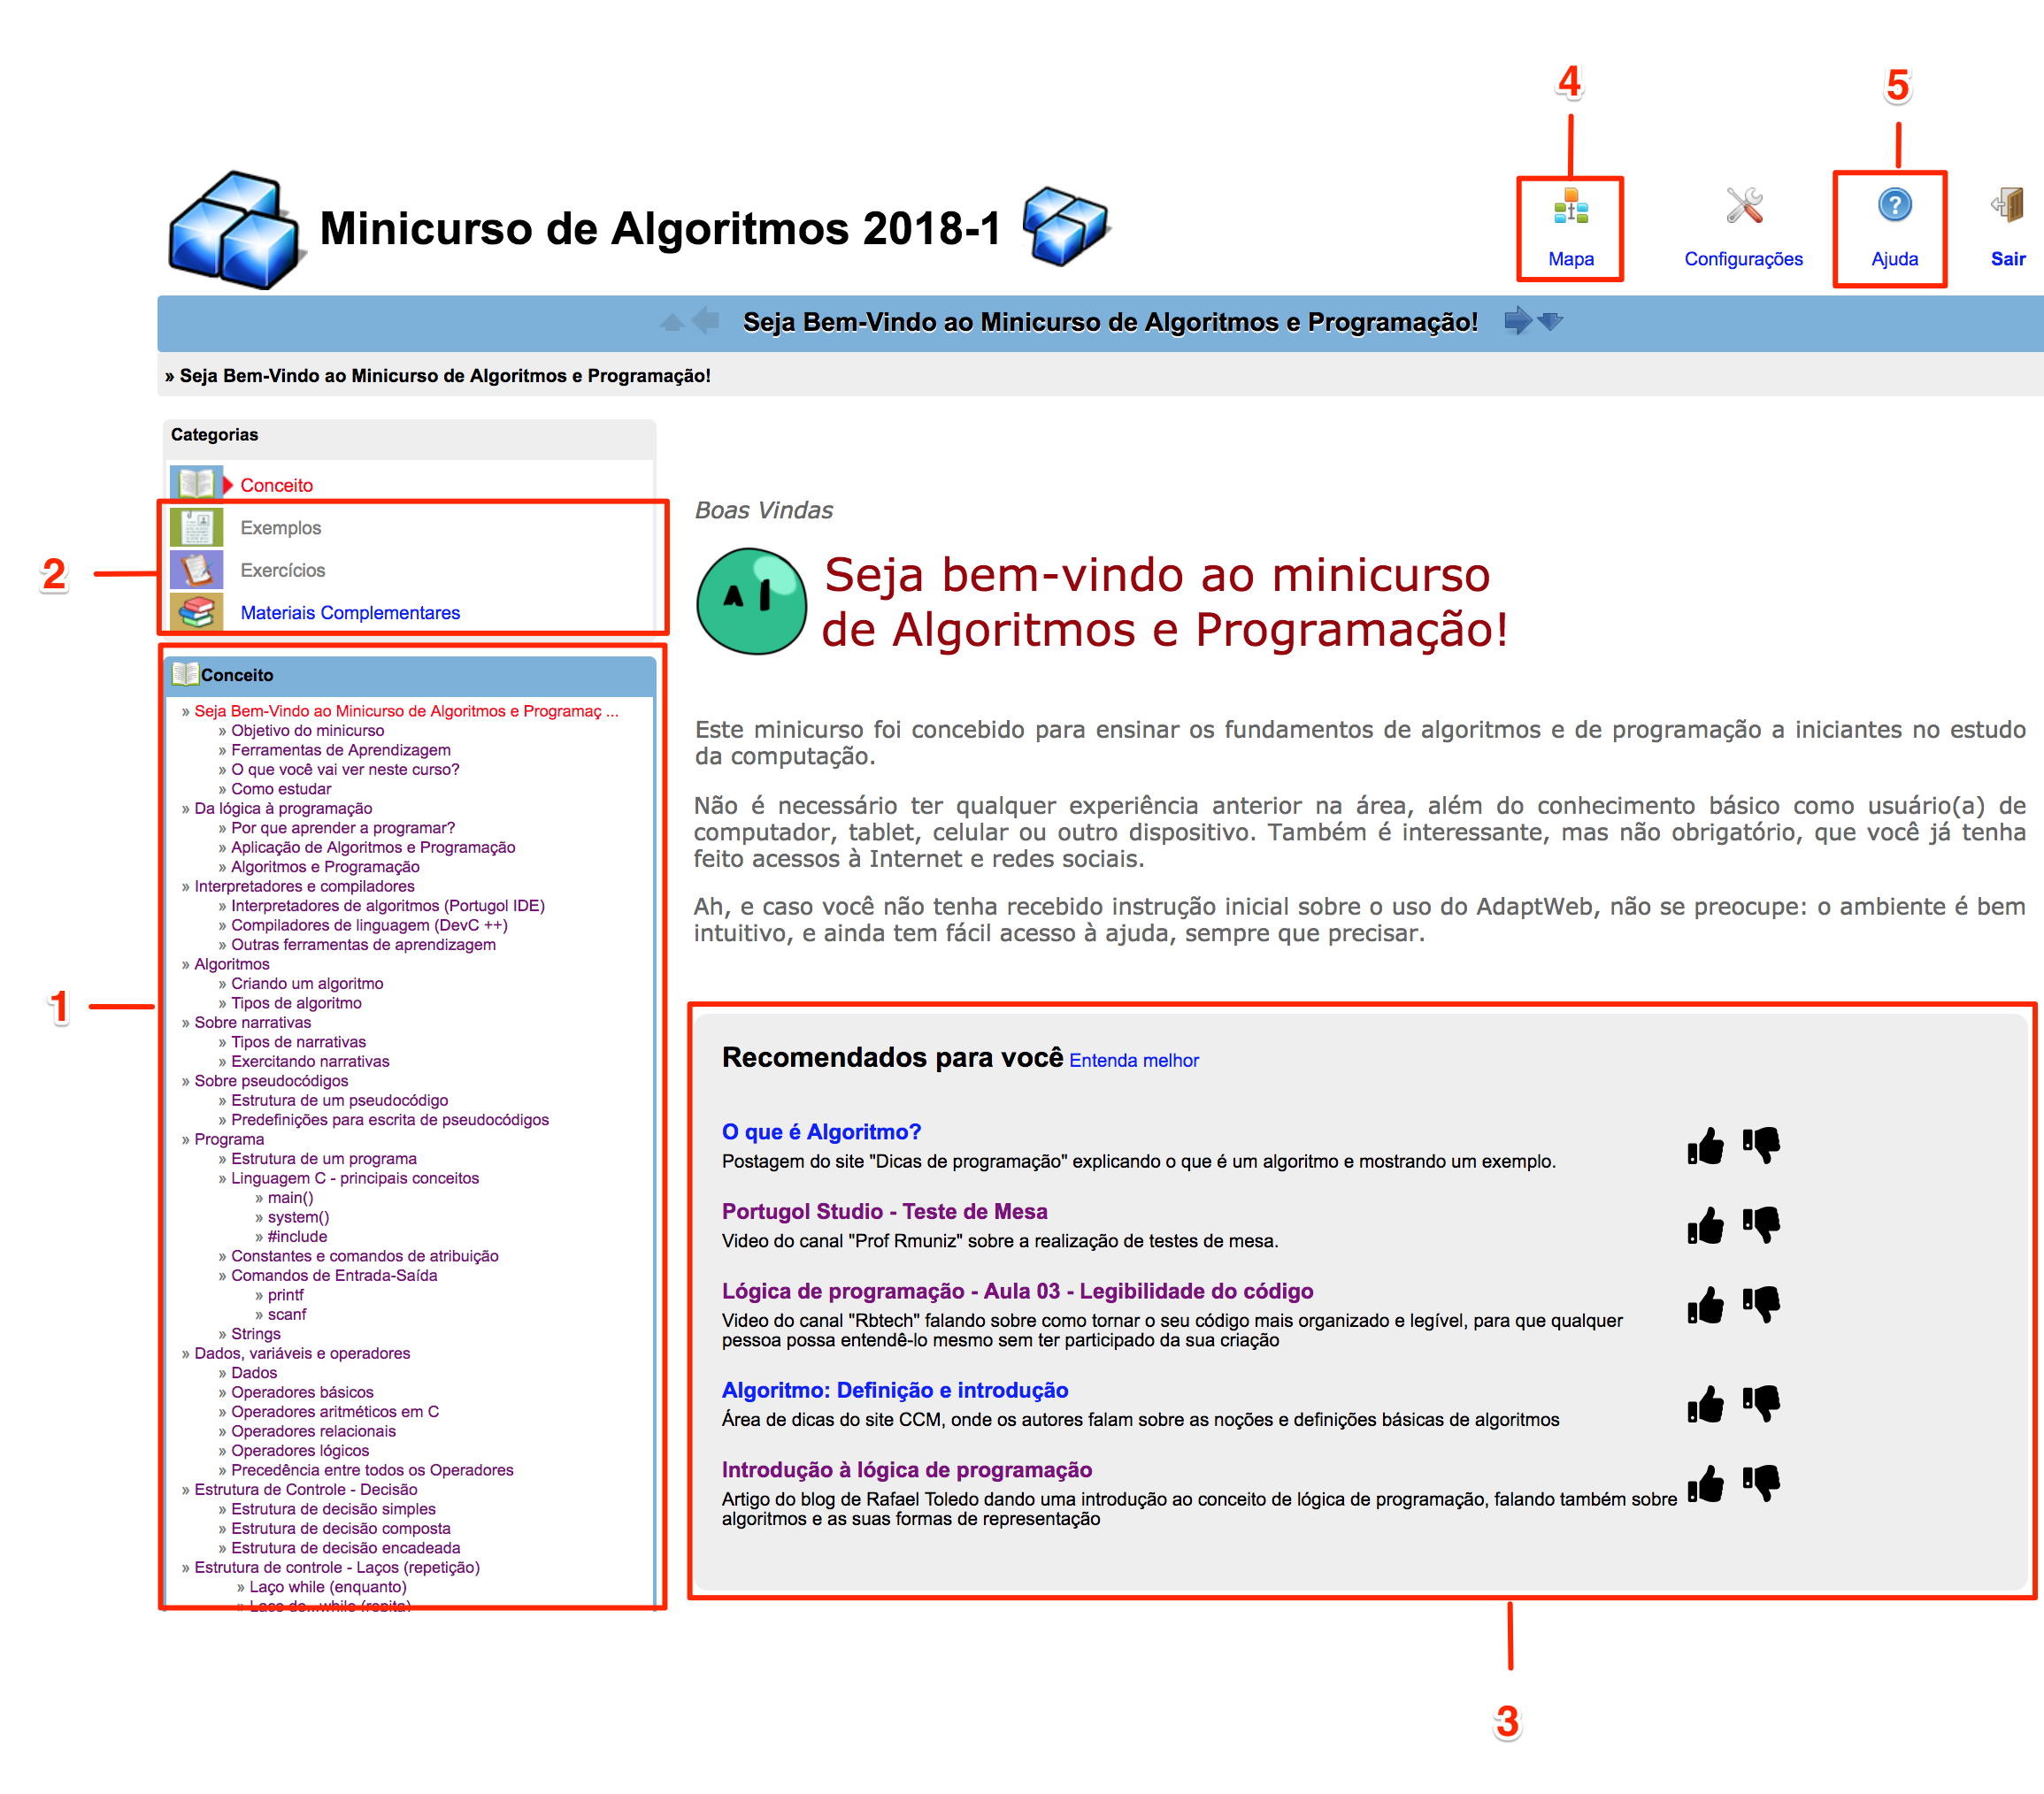
\includegraphics[scale=0.4]{./Figuras/interface-recomendacao.png}
  \end{center}
  \legend{Fonte: O autor.}
\end{figure}

Como visto na imagem, as principais informações dos Links de Apoio recomendados apresentados para o aluno são: Link, Nome do Link, Descrição e a possibilidade de avaliar o item
positivamente ou negativamente. A avaliação feita pelo usuário não é considerada pelo algoritmo de recomendação, sendo que os itens acessados pelo
usuário são considerados como do seu interesse. Como trabalho futuro é possível incorporar a avaliação na recomendação, e.g.,
não tornar a recomendar itens que foram avaliado com notas baixas ou apenas considerar para o algoritmo Baseado em Conteúdo
os itens avaliados positivamente. \citeonline{pu2012evaluating} afirmam que enquanto recomendar um item apenas é pouco, recomendar mais do que cinco itens
aumenta a dificuldade de escolhar do usuário. Por isso, a quantidade máxima de itens recomendadas para o usuário em cada
recomendação é de cinco itens.

Para cumprir o requisito de Explicação das recomendações citada por \citeonline{pu2012evaluating}, foi adicionado o
botão de "Entenda melhor" que tem por objetivo explicar ao usuário como a lista de itens foi gerada. Ao entender o
funcionamento do algoritmo de recomendação o usuário tem a possibilidade aprimorar o seu perfil para personalizar as
recomendações recebidas. Na Figura \ref{fig:adaptweb-proposta-explicacao} está um protótipo da explicação da recomendação
mostrada para o aluno.

\begin{figure}[htb]
  \caption{\label{fig:adaptweb-proposta-explicacao}Explicação da recomendação}
  \begin{center}
      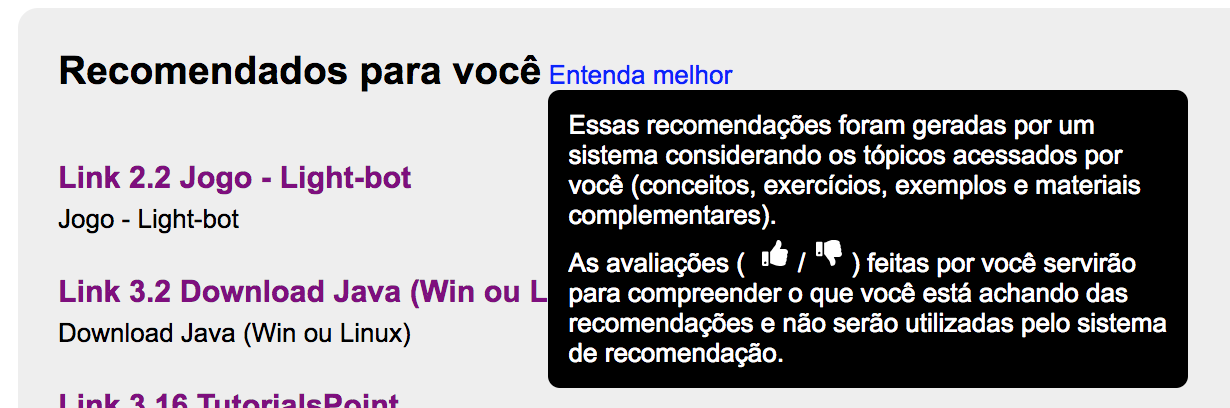
\includegraphics[scale=0.6]{./Figuras/explicacao-das-recomendacoes.png}
  \end{center}
  \legend{Fonte: O autor.}
\end{figure}

\subsection{Definição do experimento}\label{subsection:definicao-experimento}

O experimento proposto neste trabalho visa avaliar a experiência dos alunos ao interagir com o SR proposto, se comparado a um SR
utilizando a abordagem Baseada em Conteúdo tradicional. Este experimento foi
baseado nas seguintes hipóteses:

\begin{itemize}
\item \textbf{H\textsubscript{0}:} Não há diferenças na percepção do usuário da qualidade das recomendações recebidas utilizando a abordagem
Baseada em Conteúdo tradicional e a proposta desse trabalho.
\item \textbf{H\textsubscript{1}:} Há diferenças na percepção do usuário da qualidade das recomendações recebidas utilizando a abordagem
Baseada em Conteúdo tradicional e a proposta desse trabalho.
\end{itemize}

Para a execução do experimento, o SR proposto foi comparado a abordagem Baseada em Conteúdo tradicional utilizando uma
estratégia \textit{Between Subjects}, i.e., os alunos foram divididos em dois grupos e cada grupo utilizou apenas
um dos sistemas. Para garantir que a única variável seja o SR utilizado, ambos os grupos irão utilizar a mesma
interface proposta para as recomendações.

O experimento foi realizado através do Minicurso de Algoritmos e Linguagem de Programação, o qual teve seu design instrucional realizado por \citeonline{santos2017addie}.
Foram convidados a participar alunos de todos os cursos do Centro de Ciências Tecnológicas (CCT) da Universidade do
Estado de Santa Catarina (UDESC), sendo que todos os cursos do CCT possuem essa disciplina na grade curricular. Os convites
foram realizados em todas as salas das disciplinas de Algoritmos (ALG), Algoritmos e Linguagem de Programação (ALP), Linguagem
de Programação (LPG) e Iniciação a Ciência da Computação (ICC). Além disso, foi enviado um convite para todos os alunos do
campus por e-mail através da Assessoria de Comunicação e foi divulgado na página do Facebook da UDESC Joinville.

Os usuários que se matricularam no Minicurso foram aleatóriamente divididos em dois grupos, pelos mesmos critérios
utilizados por \citeonline{klockanalise}: Professor, Curso, Sexo e Idade. Isso foi possível porque durante o processo de
matrícula os alunos responderam um questionário para montar o seu perfil. Também durante a matrícula os alunos tiveram
acesso ao Termo de Consentimento Livre e Esclarecido (TCLE), presente no Apêndice \ref{ape:termo-de-consentimento}, que
explica o objetivo do experimento e no qual eles consentiram em participar e em permitir o uso dos
resultados para essa pesquisa, sempre garantindo a anonimidade dos participantes.

Ao final do minicurso, os alunos puderam acessar a avaliação do Minicurso, composta de 10 questões, e o questionário
de satisfação sobre a experiência no Minicurso em geral e com o SR. As questões relacionadas ao SR foram selecionadas do
conjunto de questões definidas por \citeonline{pu2011user} (presente no Anexo \ref{ane:questoes-framework}), para que
ficasse de acordo com o objetivo desse experimento. As questões selecionadas foram traduzidas para o português para garantir o entendimento de todos os alunos
e estão presentes no Apêndice \ref{ape:questionario-de-satisfacao}.

Durante o desenvolvimento do Minicurso foram utilizadas as Intervenções definidas por \citeonline{santos2017addie}, para
fazer com que os alunos fiquem engajados no curso. As Intervenções são e-mails combinadas com postagens no Fórum de Discussão
que guiam os alunos no seu estudo e também propõe desafios para os estudantes. As Intervenções propostas por \citeonline{santos2017addie}
consideram o Minicurso com uma duração de dois meses, por isso foi necessário uma adaptação dessas Intervenções para o período
mais reduzido no qual foi realizado esse experimento. As Intervenções adaptadas de \citeonline{santos2017addie} podem
ser vistar no Apêndice \ref{ape:intervencoes} e os Desafios postados no Fórum de Discussão estão presentes no Apêndice \ref{ane:desafios}.

\subsection{Testes piloto}\label{section:planejamento-teste-piloto}

Antes do experimento ser realizado com os alunos do CCT, foi realizado um teste piloto com
quatro alunos que já realizaram essa disciplina. O objetivo do teste piloto foi avaliar os instrumentos do experimento,
além de permitir encontrar problemas na experiência do usuário para serem corrigidos antes da execução do minicurso. O teste piloto
foi realizado no dia 06 de Abril de 2018.

Durante o teste piloto os alunos foram divididos em dois grupos aleatóriamente, sendo que dois alunos utilizaram o Sistema de Recomendação
Baseado em Conteúdo Tradicional e os outros dois utilizaram o Sistema de Recomendação com o Decaimento. Os alunos receberam
um protocolo de atividades para realizar, presente no Apêndice \ref{ape:teste-piloto}. As tarefas envolvem
realizar a matrícula na disciplina, na qual eles leram e aceitaram o TCLE, realizar o acesso a alguns conceitos e
materiais complementares, utilizar o Sistema de Recomendação, realizar a avaliação da disciplina e responder ao Questionário
de Satisfação. Durante o teste, os comentários e observações feitas pelos alunos foram anotadas para posterior análise.

Os quatro participantes do teste piloto foram identificados como Participante 1, Participante 2,
Participante 3 e Participante 4.

Os Partipantes 1 e 2 utilizaram o algoritmo tradicional de recomendação, enquanto os participantes 3 e 4 utilizaram a
proposta desse trabalho, porém eles tinham essa informação durante a realização do Teste. Os participantes foram livres na escolha do Sistema Operacional e Navegador utilizados, bem como
no Modo de Navegação escolhido (Livre ou Tutorial). A Tabela \ref{tab:participantes-teste-piloto} apresenta o
Sistema Operacional, Navegador, Modo de Navegação e o Algoritmo de Recomendação utilizado por
cada participante.

\begin{table}[h]
\footnotesize
\caption[Dados Técnicos do Participantes do Teste Piloto]{Dados Técnicos do Participantes do Teste Piloto}
\label{tab:participantes-teste-piloto}
\centering
\begin{tabular}{|p{2cm}|p{2.5cm}|p{2.5cm}|p{2.5cm}|p{2.5cm}|}
  \hline
  \textbf{Participante} & \textbf{Sistema Operacional} & \textbf{Navegador} & \textbf{Modo de Navegação} & \textbf{Algoritmo de Recomendação} \\
  \hline
  1 & Windows 7 & Firefox & Tutorial & Baseado Em Conteúdo Tradicional \\
  \hline
  2 & Windows 7 & Firefox e Chrome & Livre & Baseado Em Conteúdo Tradicional \\
  \hline
  3 & Ubuntu & Firefox & Tutorial & Baseado Em Conteúdo com Decaimento \\
  \hline
  4 & Windows 7 & Firefox & Livre & Baseado Em Conteúdo com Decaimento \\
  \hline
\end{tabular}
\legend{Fonte: O autor.}
\end{table}

Durante a execução do Teste Piloto, os participantes encontraram erros de digitação no Termo de Consentimento Livre e Esclarecido (TCLE)
e alguns problemas na prova da disciplina, como perguntas de Verdadeiro e Falso com questões duplicadas e uma
pergunta que não possuía nenhuma resposta certa. Esses problemas foram resolvidos antes do início do experimento
propriamente dito.

Os alunos também encontraram um problema de código que aconteceu em versões antigas do Firefox, por não possuir suporte a
algumas funções do \textit{JavaScript} como atrelar ações ao evento de \textit{click} de \textit{links}. O problema encontrado foi que não estavam
sendo salvas as recomendações acessadas por esses usuários no momento em que este clicava no \textit{link}, e foi confirmado
que era um problema com o Firefox, pois os próprios participantes do Teste Piloto testaram no navegador Chrome e não tiveram
o mesmo problema. Para corrigir isso, foi mudada a forma de implementação do método para salvar os \textit{clicks} nas recomendações
utilizando uma técnica chamada de \textit{Redirect Link}, na qual o usuário ao clicar na recomendação acessa primeiro um
\textit{link} interno ao \adaptweb que salva qual o \textit{link} acessado e depois redireciona o usuário para o \textit{link} externo.
Dessa forma, a implementação não depende do suporte ao \textit{JavaScript} e pode ser acessado por qualquer versão de navegador.

Sobre as recomendações, os Participantes 1 e 2 comentaram que aparentemente os Links de Apoio recomendados para eles não
mudaram muito durante toda a interação. As vezes mudavam de ordem apenas, porém continuavam os mesmo itens. Já os Participantes
3 e 4 comentaram que ao acessar um novo conceito pelo menos 3 novos Links eram recomendados, enquanto os outros dois continuavam
os mesmos da tela anterior. Esse resultado demonstra o problema da Superespecilização presente na Abordagem Baseada em Conteúdo Tradicional,
e mostra um indício de que a proposta desse trabalho utilizando o Decaimento diminui consideravelmente esse problema.

Os participantes também observaram que desde o primeiro acesso a disciplina eles receberam cinco links com recomendação, i.e.,
o número máximo possível. Isso mostra que, como não foi definido um limiar mínimo para a similaridade entre o perfil do usuário
e os Links de Apoio, mesmo que a similaridade seja muito pequena o algoritmo sempre irá recomendar algo para o aluno. Por
outro lado, não seria interessante adicionar um limiar para o experimento deste trabalho pois estaria adicionando uma
variável interveniente. Como trabalho futuro é possível analisar como o limiar mínimo para a similaridade pode afetar
a qualidade percebida das recomendações.

A Tabela \ref{tab:teste-piloto-dados-de-uso} apresenta os dados de uso de cada Participante do Teste Piloto. Os Itens Acessados
representam os Conceitos, Materiais Complementares e Links de Apoio acessados pelo usuário. Os Links de Apoio acessados
representam as recomendações e as recomendações geradas representam quantas vezes a página acessada pelos usuários apresentou
a área de recomendações. Esse número tende a ser mais alto pois todas as páginas de Conceitos e Materiais Complementares
apresentam a área das recomendações.

\begin{table}[h]
\footnotesize
\caption[Teste Piloto: Dados de Uso]{Teste Piloto: Dados de Uso}
\label{tab:teste-piloto-dados-de-uso}
\centering
\begin{tabular}{|p{2cm}|p{3cm}|p{3cm}|p{3cm}|}
  \hline
  \textbf{Participante} & \textbf{Itens Acessados} & \textbf{Links de Apoio Acessados} & \textbf{Recomendações Geradas} \\
  \hline
  1            & 52              & -                        & 53                    \\
  \hline
  2            & 106             & 5                        & 105                   \\
  \hline
  3            & 29              & 8                        & 23                    \\
  \hline
  4            & 58              & -                        & 64                    \\
  \hline
\end{tabular}
\end{table}

Os Participantes 1 e 4 não tiveram nenhum Link de Apoio Acessado por conta do problema citado anteriormente com o navegador
Firefox numa versão mais antiga. O Participante 2 teve o mesmo problema, mas depois mudou para o Google Chrome e teve os
seus acessos salvos. Além disso, é possível observar que o número de itens foram acessados pelos participantes é bastante
similar ao número de recomendações geradas. Isso porque as principais páginas do ambiente do aluno são salvas como Item acessado
e também geram recomendação.

Ao final do Teste Piloto foi realizada uma pequena entrevista com os participantes onde eles afirmaram ter entendido e gostado
da interface do Sistema de Recomendação. Quando revelado que cada participante fazia parte de um grupo diferente e que eles
não estavam todos utilizando o mesmo Sistema de Recomendação, os participantes associaram essa informação com os
comentários que tinham feito anteriormente sobre a repetição dos itens por alguns e a novidade nas recomendações por outros.

\section{Execução}\label{section:execucao-experimento}

O período de matrícula para o minicurso 09 de Abril de 2018 até 13 de Abril de 2018. Durante esse período, todas as turmas
das disciplinas mencionadas na Seção \ref{subsection:definicao-experimento} foram visitadas, convidando os alunos a se matricular no minicurso.

No total, 208 alunos se matricularam no Minicurso. Esses alunos foram homogeneamente divididos em dois grupos utilizando os
seguintes critérios: Professor, Curso, Sexo e Idade. A Tabela \ref{tab:divisao-alunos-experimento} mostra o resultado da divisão dos alunos.

\begin{table}[ht]
\footnotesize
\caption[Divisão dos alunos de acordo com os critérios]{Divisão dos alunos de acordo com os critérios}
\label{tab:divisao-alunos-experimento}
\centering
\begin{tabular}{ccccc}
  \hline
  \multicolumn{2}{c}{\multirow{2}{*}{\textbf{Critério}}}           & \multirow{2}{*}{\textbf{Total}}           & \multicolumn{2}{c}{\textbf{Algoritmo de Recomendação}} \\
                                        &                          &                                           & Tradicional          & Proposta                        \\
  \hline
  \multirow{12}{*}{Professor}           & Professor A              & 12                                        & 6                    & 6                               \\
                                        & Professor B              & 18                                        & 9                    & 9                               \\
                                        & Professor C              & 7                                         & 4                    & 3                               \\
                                        & Professor D              & 5                                         & 3                    & 2                               \\
                                        & Professor E              & 38                                        & 19                   & 19                              \\
                                        & Professor F              & 4                                         & 2                    & 2                               \\
                                        & Professor G              & 10                                        & 5                    & 5                               \\
                                        & Professor H              & 6                                         & 3                    & 3                               \\
                                        & Professor I              & 6                                         & 3                    & 3                               \\
                                        & Professor J              & 26                                        & 13                   & 13                              \\
                                        & Professor K              & 14                                        & 7                    & 7                               \\
                                        & Outro                    & 52                                        & 30                   & 32                              \\
  \hline
  \multirow{9}{*}{Curso}                & Computação               & 55                                        & 23                   & 22                              \\
                                        & TADS                     & 36                                        & 18                   & 18                              \\
                                        & Elétrica                 & 36                                        & 18                   & 18                              \\
                                        & Física                   & 10                                        & 5                    & 5                               \\
                                        & Mecânica                 & 31                                        & 15                   & 16                              \\
                                        & Química                  & 3                                         & 2                    & 1                               \\
                                        & Produção                 & 20                                        & 10                   & 10                              \\
                                        & Civil                    & 15                                        & 7                    & 8                               \\
                                        & Matematica               & 12                                        & 6                    & 6                               \\
  \hline
  \multirow{3}{*}{Sexo}                 & Masculino                & 135                                       & 67                   & 68                              \\
                                        & Feminino                 & 72                                        & 36                   & 36                              \\
                                        & Não informado            & 1                                         & 1                    & 0                               \\
  \hline
  \multirow{6}{*}{Idade}                & Até 17 anos              & 21                                        & 10                   & 11                              \\
                                        & 18 ou 19 anos            & 75                                        & 37                   & 38                              \\
                                        & 20 ou 21 anos            & 35                                        & 18                   & 17                              \\
                                        & 22 ou 23 anos            & 11                                        & 6                    & 5                               \\
                                        & 24 ou 25 anos            & 26                                        & 13                   & 13                              \\
                                        & 26 anos ou mais          & 40                                        & 20                   & 20                              \\
  \hline
                                        & Total                    & 208                                       & 104                  & 104                             \\
  \hline
\end{tabular}
\end{table}

O período de execução do Minicurso foi de 16 de Abril de 2018 até 10 de Maio de 2018. Nesse período, dos 208 alunos
matriculados no Minicurso, 145 acessaram a disciplina pelo menos uma vez, sendo 76 do grupo estava
utilizando o algoritmo Tradicional de recomendação e 69 que utilizaram a Proposta desse trabalho.

O período para realizar a prova da disciplina e responder ao questionário de satisfação foi de 11 de Maio de 2018 até
14 de Maio de 2018. Nesse período, dos 145 alunos que acessaram a disciplina pelo menos uma vez, 85 realizaram a prova final e responderam ao
questionário de satisfação, sendo 48 do grupo que utilizou o algoritmo Tradicional e 37 do grupo que utilizou a Proposta
com decaimento. Dos 85 alunos que finalizaram a disciplina (i.e., realizaram a prova e responderam ao questionário de
satisfação), 47 acessaram pelo menos uma recomendação que recebeu, sendo 25 do grupo utilizou a abordagem Tradiconal e
22 que utilizaram a Proposta desse trabalho. A Tabela \ref{tab:uso-minicurso-sr} apresenta mais alguns dados, além dos
comentados anteriormente, como: (1) a quantidade de usuários que avaliaram as recomendações que acessaram;
(2) quantidade de recomendações acessadas; (3) quantidade de recomendações avaliadas positivamente; etc.

\begin{table}[h]
\centering
\caption{Uso do Minicurso de Algoritmos e do Sistema de Recomendação}
\label{tab:uso-minicurso-sr}
\begin{tabular}{|p{7.5cm}|p{2.5cm}|p{2.5cm}|p{2.5cm}|}
\hline
\textbf{Quantidade de:}                                                                     & \textbf{Tradicional} & \textbf{Proposta}    & \textbf{Total}    \\
\hline
Alunos que se matricularam                                                                  & 104                  & 104                  & 208      \\
\hline
Alunos que entraram pelo menos uma vez no curso                                             & 76                   & 69                   & 145      \\
\hline
Alunos que acessaram pelo menos uma recomendação                                            & 46                   & 39                   & 85       \\
\hline
Alunos que avaliaram pelo menos uma recomendação                                            & 30                   & 22                   & 52       \\
\hline
Alunos que responderam a avaliação                                                          & 48                   & 38                   & 86       \\
\hline
Alunos que responderam o questionário de satisfação                                         & 48                   & 37                   & 85       \\
\hline
Alunos que responderam o questionário de satisfação e acessaram pelo menos uma recomendação & 25                   & 22                   & 47       \\
\hline
Alunos que responderam o questionário de satisfação e avaliaram pelo menos uma recomendação & 16                   & 13                   & 29       \\
\hline
Acessos aos itens recomendados                                                              & 227                  & 396                  & 623      \\
\hline
Avaliações positivas ao itens recomendados                                                  & 141                  & 234                  & 375      \\
\hline
Avaliações negativas ao itens recomendados                                                  & 5                    & 4                    & 9        \\
\hline
\end{tabular}
\end{table}

Pela Tabela \ref{tab:uso-minicurso-sr} podemos perceber que 38 alunos que responderam ao questionário não acessaram nenhuma
recomendação, sendo 23 do grupo que utilizou o algoritmo Tradicional e 15 do grupo que utilizou a Proposta desse
trabalho. Na Subseção \ref{subsection:analise-uso-sr} os dados de acesso e avaliação das recomendações são analisadas mais profundamente,
comparando os resultados dos dois algoritmos utilizando técnicas estatísticas descritas na Subseção \ref{section:tecnicas-analise-estatistica}.

\section{Análise dos Resultados}\label{section:analise-experimento}

Nessa Seção são descritas as análises estatísticas realizadas sobre os dados coletados durante a execução do experimento.
As técnicas estatísticas utilizadas para fazer a análise são apresentadas na Subseção \ref{section:tecnicas-analise-estatistica}
e nas Subseções subsequentes são apresentas as análises realizadas no questionário de satisfação e nos dados de acesso
dos alunos.

\subsection{Técnicas de Análise Estatística}\label{section:tecnicas-analise-estatistica}

Para realizar as análises estatísticas, primeiro foi necessário entender os tipos de variáveis que podem ser analisadas.
As variáveis são as informações coletadas durante o experimento e podem ser quantitativas ou qualitativas \cite{bussab2012morettin}.
As variváveis quantitativas são resultado de uma contagem e/ou mensuração \cite{bussab2012morettin} e podem ser discretas
(conjunto finito ou enumerável de números) ou contínuas (pertencem a um intervalo de números reais). Exemplos de variáveis
quantitativas são número de filhos, número de cômodos em uma casa, número de pessoas presentes em uma sala, altura e peso.
As variáveis qualitativas são aquelas que descrevem um aspecto relacionado ao objeto estudado \cite{bussab2012morettin} e podem ser
nominais (quando não possuem ordenação) ou ordinais (quando há ordem entre os valores). Exemplos de variáveis qualitativas
são sexo, estado civil e grau de instrução.

A variável independente desse trabalho é o algoritmo de recomendação utilizado pelo alunos, que pode assumir os valores
"Baseado em Conteúdo Tradicional" ou "Baseado em Conteúdo com Decaimento". As variáveis dependentes analisadas são o grau de
satisfação do alunos em relação ao Sistema de Recomendação, a quantidade de recomendações utilizadas pelos alunos, a quantidade de recomendações
avaliadas positiva ou negativamente pelos alunos e a Precisão do algoritmo de recomendação. O grau de satisfação pode ser
categorizado como uma variável qualitativa ordinal, pois os alunos indicaram a sua satisfação respondendo a um questionário
com questão com escala de Likert. A quantidade de recomendações acessadas e/ou avaliadas são variáveis quantitativas discretas,
enquanto a Precisão do algoritmo de recomendação é uma variável quantitativa contínua.

De acordo com o tipo de variável analisado e a distribuição dos valores dessa variável é possível definir qual técnica
estatística será utilizada. O fluxograma da Figura \ref{fig:fluxograma-tecnica-moissa} produzido por \citeonline{moissa2016influencia}
define como decidir as técnicas estatísticas utilizadas.

\begin{figure}[htb]
  \caption{\label{fig:fluxograma-tecnica-moissa}Fluxograma de uso das técnicas estatísticas}
  \begin{center}
      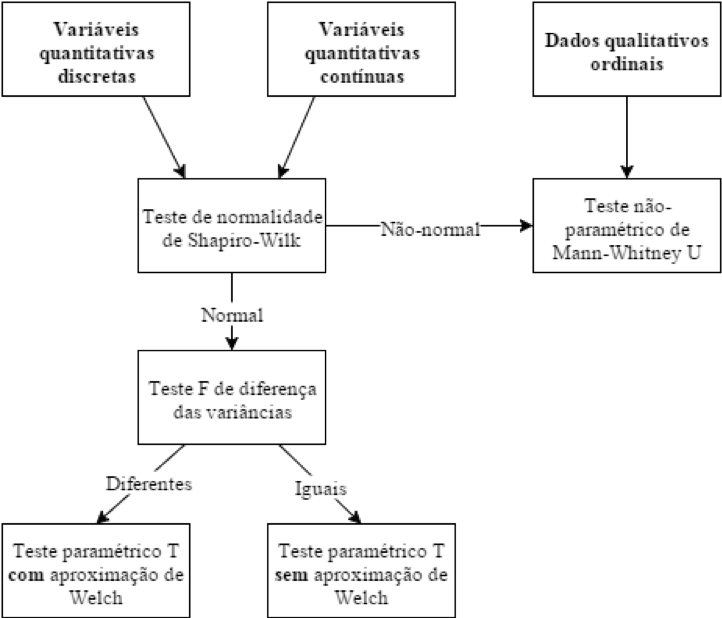
\includegraphics[scale=1.0]{./Figuras/fluxograma-tecnicas-moissa.png}
  \end{center}
  \legend{Fonte: \citeonline{moissa2016influencia}}
\end{figure}

Conforme o fluxograma na Figura \ref{fig:fluxograma-tecnica-moissa}, quando a variável é quantitativa (discreta ou contínua)
é realizado um teste de normalidade para verificar a distribuição dos valores. Se o resultado mostrar uma distribuição
normal é realizado o teste F para verificar a variância das amostras. Se o resultado do teste F mostrar que as variâncias
são diferentes a Aproximação de Welch será utilizada no teste T, caso contrário o teste T é aplicado sem a Aproximação de Welch.
Se o resultado do teste de normalidade mostrar uma distribuição não-normal é adotado o teste não paramétrico de
Mann-Whitney U. Este teste também é utilizado para todas as variáveis qualitativas ordinais, pois estas variáveis devem
ser analisadas através de testes não-paramétricos \cite{moissa2016influencia}.

Todos os testes mencionados estão disponíveis na ferramenta estatística R, que foi a ferramenta utilizada para todas as análises
realizadas nas Subseções a seguir.

\subsection{Análise do Questionário de Satisfação}\label{subsection:analise-questionario-satisfacao}

O Questionário de Satisfação aplicado ao final do Minicurso de Algoritmos tem o objetivo de identificar a percepção dos
alunos sobre a qualidade das recomendações e também da interface do Sistema de Recomendação em si. As questões do questionário
podem ser vistas no Apêndice \ref{ape:questionario-de-satisfacao} e possui 13 questões, divididas em 7 categorias. Todas
as questões foram selecionadas do questionário definido por \citeonline{pu2011user} (presente no Anexo \ref{ane:questoes-framework})
e traduzidas para o Português. Essas questões são afirmações nas quais os alunos devem se posicionar em uma escala de
Likert de cinco pontos, de "Discordo Totalmente" até "Concordo Totalmente". Também foi adicionada uma opção de "Não utilizei" para
os alunos que não utilizaram o Sistema de Recomendação (ou usaram sem perceber). A Tabela \ref{tab:questionario-satisfacao-respostas}
apresenta as respostas agrupadas dos alunos para cada uma das perguntas.

\begin{table}[h]
\footnotesize
\caption{Respostas ao Questionário de Satisfação}
\label{tab:questionario-satisfacao-respostas}
\centering
\begin{tabular}{|p{1.5cm}|p{1.8cm}|p{2.2cm}|p{0.6cm}|p{0.6cm}|p{0.6cm}|p{2.3cm}|p{2cm}|}
\hline
\textbf{Questão} & \textbf{Algoritmo}   & \textbf{Discordo tot.} & \textbf{-} & \textbf{-} & \textbf{-} & \textbf{Concordo tot.} & \textbf{Não utilizei} \\
\hline
\multirow{2}{*}{1}          & Tradicional & 2                   & 1                     & 2                         & 15                    & 11                  & 17           \\
                            & Proposta    & 0                   & 0                     & 6                         & 11                    & 7                   & 13           \\
\hline
\multirow{2}{*}{2}          & Tradicional & 1                   & 0                     & 5                         & 18                    & 6                   & 18           \\
                            & Proposta    & 0                   & 1                     & 7                         & 9                     & 9                   & 11           \\
\hline
\multirow{2}{*}{3}          & Tradicional & 2                   & 0                     & 8                         & 13                    & 8                   & 17           \\
                            & Proposta    & 0                   & 2                     & 4                         & 12                    & 8                   & 11           \\
\hline
\multirow{2}{*}{4}          & Tradicional & 1                   & 0                     & 5                         & 17                    & 6                   & 19           \\
                            & Proposta    & 0                   & 1                     & 8                         & 8                     & 10                  & 10           \\
\hline
\multirow{2}{*}{5}          & Tradicional & 3                   & 0                     & 4                         & 10                    & 10                  & 21           \\
                            & Proposta    & 0                   & 2                     & 9                         & 8                     & 6                   & 12           \\
\hline
\multirow{2}{*}{6}          & Tradicional & 3                   & 3                     & 3                         & 12                    & 8                   & 19           \\
                            & Proposta    & 0                   & 0                     & 5                         & 11                    & 10                  & 11           \\
\hline
\multirow{2}{*}{7}          & Tradicional & 2                   & 5                     & 4                         & 14                    & 9                   & 14           \\
                            & Proposta    & 1                   & 1                     & 7                         & 9                     & 7                   & 12           \\
\hline
\multirow{2}{*}{8}          & Tradicional & 0                   & 6                     & 3                         & 12                    & 9                   & 18           \\
                            & Proposta    & 0                   & 2                     & 8                         & 8                     & 6                   & 13           \\
\hline
\multirow{2}{*}{9}          & Tradicional & 2                   & 2                     & 7                         & 10                    & 7                   & 20           \\
                            & Proposta    & 0                   & 0                     & 11                        & 5                     & 8                   & 13           \\
\hline
\multirow{2}{*}{10}         & Tradicional & 1                   & 0                     & 10                        & 14                    & 4                   & 19           \\
                            & Proposta    & 0                   & 2                     & 4                         & 12                    & 8                   & 11           \\
\hline
\multirow{2}{*}{11}         & Tradicional & 2                   & 2                     & 6                         & 13                    & 5                   & 20           \\
                            & Proposta    & 0                   & 1                     & 6                         & 10                    & 8                   & 12           \\
\hline
\multirow{2}{*}{12}         & Tradicional & 4                   & 1                     & 6                         & 17                    & 2                   & 18           \\
                            & Proposta    & 0                   & 1                     & 5                         & 9                     & 10                  & 12           \\
\hline
\multirow{2}{*}{13}         & Tradicional & 2                   & 0                     & 6                         & 13                    & 12                  & 15           \\
                            & Proposta    & 0                   & 1                     & 4                         & 7                     & 14                  & 11           \\
\hline
\end{tabular}
\end{table}

Através das respostas dos alunos presentes na Tabela \ref{tab:questionario-satisfacao-respostas}, podemos perceber que
os alunos que utilizaram a abordagem Baseada em Conteúdo Tradicional tiveram mais respostas de "Discordo Totalmente" do
que os alunos utilizaram a abordagem Com Decaimento, com 25 para o algoritmo Tradicional e uma para a proposta desse trabalho.
Além disso, podemos perceber que 12 questões tiveram pelo menos um "Discordo Totalmente" para o grupo que utilizou o algoritmo
Tradicional e uma questão para o grupo que utilizou a Proposta Com Decaimento.

Com relação a resposta "Concordo Totalmente", tiveram 97 respostas para o grupo que utilizou o algoritmo Tradicional e 111
para o grupo que utilizou a proposta desse trabalho. O resultado das respostas "Não utilizei" mostram que os alunos responderam
que não utilizaram para apenas algumas perguntas e não para todas, sendo que para o grupo
que utilizou o algoritmo Tradicional o valor varia entre 17 e 21 alunos e para o grupo que utilizou a Proposta desse
trabalho variou entre 10 e 13 alunos. O fato desse valor ter variado tanto não foi esperado inicialmente, mas podemos afirmar que pelo menos 17 alunos do primeiro grupo e 10 alunos do segundo grupo
não utilizaram ter utilizado o Sistema de Recomendação. Ao comparar essa informação com os dados de acesso
dos alunos, que diz que 23 alunos do grupo Tradicional e 15 alunos do grupo Com Decaimento não acessaram nenhuma recomendação,
é provável que apesar de não terem acessado nenhuma recomendação os alunos perceberam o Sistema de Recomendação e analisaram
as recomendações recebidas.

As respostas dadas ao questionário de satisfação foram analisadas utilizando teste não paramétrico de
Mann-Whitney U para verificar se existe diferença estatisticamente significativa entre as respostas dos dois grupos (i.e., \textit{p} < 0.05).
As respostas de "Não utilizei" não foram consideradas nessa análise. O resultado das análises está presente no Apêndice
\ref{ape:analise-estatistica-questionario}. Essa análise mostrou que, apesar da aparente diferença nas respostas dadas
pelos alunos favorável à proposta desse trabalho, apenas uma questão apresentou uma diferença significativa entre as
respostas dos dois grupos. Isso se deve ao fato de ter mais respostas em "Discordo Parcialmente",
"Não Concordo e Nem Discordo" e "Concordo Parcialmente" para o grupo do algoritmo Tradicional do que para o grupo da
Proposta desse trabalho, com 248 para o primeiro e 217 para o segundo, que equilibrou os resultados dos dois grupos.

A única questão que apresentou diferença significativa foi a questão 12 (i.e., "Eu entendi porque os
itens foram recomendados para mim.") e foi favorável à proposta desse trabalho. A diferença significativa nessa questão
mostra que os alunos que utilizaram o algoritmo Com Decaimento puderam perceber melhor a relação entre os itens que acessaram
com os links que foram recomendados do que os alunos que utilizaram a abordagem Tradicional.

\subsection{Análise do uso do SR}\label{subsection:analise-uso-sr}

\section{Outras Análises}\label{section:outras-analises}

\section{Considerações sobre o capítulo}

Neste capítulo foi descrito o ambiente no qual o Sistema de Recomendação (SR) proposto será incorporado (\adaptweb) e definido o
experimento para a avaliação da proposta desse trabalho. Nos SRs desenvolvidos no \adaptweb, tanto para a proposta deste trabalho como para a abordagem
Baseada em Conteúdo tradicional que será utilizada como parâmetro, o perfil do usuário é composto pelo conjunto de palavras-chave de todos os itens acessados pelo usuário, das
cinco categorias apresentadas. Os itens a serem recomendados são os Links de Apoio, visto que os itens das outras categorias
são estruturados pelo professor e estão fortemente relacionados à conceitos específicos.

Utilizando como base as diretrizes propostas por \citeonline{pu2012evaluating} foi proposta uma interface para a apresentação das recomendações no \adaptweb,
com o objetivo de que os usuários tenham acesso direto as recomendações na tela principal do ambiente do aluno e entendam
melhor o porque aqueles itens foram recomendados. Como visto, essa interface será utilizada tanto pelo algoritmo proposto
quanto pela abordagem tradicional.

O experimento visa avaliar a experiência do usuário com o SR proposto no Capítulo \ref{chapter:proposta} em
comparação à abordagem Baseada em Conteúdo tradicional. O experimento acontecerá no ambiente
\adaptweb através de um minicurso de algoritmos desenvolvido no ambiente nos meses de
Abril e Maio de 2018. Ao final do minicurso os alunos receberão um questionário para responder sobre a sua experiência
ao interagir com o SR, que será adaptado do conjunto de questões definidas por \citeonline{pu2011user}. Ao final do
experimento, espera-se chegar a uma conclusão se existe diferença na percepção do usuário sobre a qualidade
das recomendações recebidas ao utilizar um SR Sensível ao Tempo, que se adapta as variações de interesse do
aluno, em relação a uma abordagem tradicional de recomendação.

\chapter{Resultados}\label{chapter:resultados}

Esse capítulo apresenta os resultados do Teste Piloto e do Experimento descritos no Capítulo \ref{chapter:experimento}.
A Seção \ref{section:resultados-teste-piloto} apresenta os resultados do Teste Piloto enquanto a Seção \ref{section:resultados-experimento}
apresenta os resultados do experimento, através do Questionário de Satisfação aplicado ao final do experimento e da Ánalise
de Uso do Sistema de Recomendação.

\section{Teste Piloto}\label{section:resultados-teste-piloto}

Como dito na Seção \ref{section:planejamento-teste-piloto}, quatro alunos que já realizaram a disciplina de Algoritmos e
Linguagem de Programação participaram do Teste Piloto. Aqui eles serão identificados como Participante 1, Participante 2,
Participante 3 e Participante 4.

Os Partipantes 1 e 2 utilizaram o algoritmo tradicional de recomendação, enquanto os participantes 3 e 4 utilizaram a
proposta desse trabalho, porém eles tinham essa informação durante a realização do Teste. Os participantes foram livres na escolha do Sistema Operacional e Navegador utilizados, bem como
no Modo de Navegação escolhido (Livre ou Tutorial). A Tabela \ref{tab:participantes-teste-piloto} apresenta o
Sistema Operacional, Navegador, Modo de Navegação e o Algoritmo de Recomendação utilizado por
cada participante.

\begin{table}[h]
\footnotesize
\caption[Dados Técnicos do Participantes do Teste Piloto]{Dados Técnicos do Participantes do Teste Piloto}
\label{tab:participantes-teste-piloto}
\centering
\begin{tabular}{|p{2cm}|p{2.5cm}|p{2.5cm}|p{2.5cm}|p{2.5cm}|}
  \hline
  \textbf{Participante} & \textbf{Sistema Operacional} & \textbf{Navegador} & \textbf{Modo de Navegação} & \textbf{Algoritmo de Recomendação} \\
  \hline
  1 & Windows 7 & Firefox & Tutorial & Baseado Em Conteúdo Tradicional \\
  \hline
  2 & Windows 7 & Firefox e Chrome & Livre & Baseado Em Conteúdo Tradicional \\
  \hline
  3 & Ubuntu & Firefox & Tutorial & Baseado Em Conteúdo com Decaimento \\
  \hline
  4 & Windows 7 & Firefox & Livre & Baseado Em Conteúdo com Decaimento \\
  \hline
\end{tabular}
\legend{Fonte: O autor.}
\end{table}

Durante a execução do Teste Piloto, os participantes encontraram erros de digitação no Termo de Consentimento Livre e Esclarecido (TCLE)
e alguns problemas nas questões da avaliação da disciplina, como perguntas de Verdadeiro e Falso com questões duplicadas e uma
questão que não possuía nenhuma resposta certa. Esses problemas encontrados foram resolvidos antes do início do experimento
desse trabalho.

Os alunos também encontraram um problema de código que aconteceu em versões antigas do Firefox, por não possuir suporte a
algumas funções do \textit{JavaScript} como atrelar ações ao evento de \textit{click} de \textit{links}. O problema encontrado foi que não estavam
sendo salvas as recomendações acessadas por esses usuários no momento em que este clicava no \textit{link}, e foi confirmado
que era um problema com o Firefox pois os próprios participantes do Teste Piloto testaram no navegador Chrome e não tiveram
o mesmo problema. Para corrigir isso, foi mudada a forma de implementação do método para salvar os \textit{clicks} nas recomendações
utilizando uma técnica chamada de \textit{Redirect Link}, na qual o usuário ao clicar na recomendação acessa primeiro um
\textit{link} interno ao \adaptweb que salva qual o \textit{link} acessado e depois redireciona o usuário para o \textit{link} externo corretamente.
Dessa forma, a implementação não depende do suporte ao \textit{JavaScript} e pode ser acessado por qualquer versão de navegadores.

Sobre as recomendações, os Participantes 1 e 2 comentaram que aparentemente os Links de Apoio recomendados para eles não
mudaram muito durante toda a interação. As vezes mudavam de ordem apenas, porém continuavam os mesmo itens. Já os Participantes
3 e 4 comentaram que ao acessar um novo conceito pelo menos 3 novos Links era recomendados, enquanto os outros dois continuavam
os mesmos da tela anterior. Esse resultado é um indício da Superespecilização presente na Abordagem Baseada em Conteúdo Tradicional,
e mostra que a proposta desse trabalho utilizando o Decaimento diminui consideravelmente esse problema.

Os Participantes também observaram que desde o primeiro acesso a disciplina eles receberam cinco links com recomendação, i.e.,
o número máximo possível. Isso mostra que, como não foi definido um limiar mínimo para a similaridade entre o perfil do usuário
e os Links de Apoio, mesmo que a similaridade seja muito pequena o algoritmo sempre irá recomendar algo para o aluno. Por
outro lado, não seria interessante adicionar um limiar para o experimento deste trabalho pois estaria adicionando uma
variável interveniente. Como trabalho futuro é possível analisar como o limiar mínimo para a similaridade pode afetar
a qualidade percebida das recomendações.

A Tabela \ref{tab:teste-piloto-dados-de-uso} apresenta os dados de uso de cada Participante do Teste Piloto. Os Itens Acessados
representam os Conceitos, Materiais Complementares e Links de Apoio acessados pelo usuário. Os Links de Apoio acessados
representam as recomendações e as recomendações geradas representam quantas vezes a página acessada pelos usuários apresentou
a área de recomendações. Esse número tende a ser mais alto pois todas as páginas de Conceitos e Materiais Complementares
apresentam a área das recomendações.

\begin{table}[h]
\footnotesize
\caption[Teste Piloto: Dados de Uso]{Teste Piloto: Dados de Uso}
\label{tab:teste-piloto-dados-de-uso}
\centering
\begin{tabular}{|p{2cm}|p{3cm}|p{3cm}|p{3cm}|}
  \hline
  \textbf{Participante} & \textbf{Itens Acessados} & \textbf{Links de Apoio Acessados} & \textbf{Recomendações Geradas} \\
  \hline
  1            & 52              & -                        & 53                    \\
  \hline
  2            & 106             & 5                        & 105                   \\
  \hline
  3            & 29              & 8                        & 23                    \\
  \hline
  4            & 58              & -                        & 64                    \\
  \hline
\end{tabular}
\end{table}

Os Participantes 1 e 4 não tiveram nenhum Link de Apoio Acessado por conta do problema citado anteriormente com o navegador
Firefox numa versão mais antiga. O Participante 2 teve o mesmo problema, mas depois mudou para o Google Chrome e teve os
seus acessos salvos. Além disso, é possível observar que o número de itens foram acessados pelos participantes é bastante
similar ao número de recomendações geradas. Isso porque geralmente um Item acessado está associado ao acesso de uma página
do Minicurso que também gera recomendações, porém também é possível na página de Materiais Complementares de um Tópico o usuário
gerar recomendação e não acessar nenhum material ou acessar mais de material. Por isso, a diferença nos números.

Ao final do Teste Piloto foi realizada uma pequena entrevista com os participantes onde eles afirmaram ter entendido e gostado
da interface do Sistema de Recomendação. Quando revelado que cada participante fazia parte de um grupo diferente e que eles
não estavam todos utilizando o mesmo Sistema de Recomendação os participantes associaram com os comentários que tinham feito
anteriormente sobre a repetição dos itens por alguns e a novidade nas recomendações por outros.

\section{Experimento}\label{section:resultados-experimento}

Ids para nao considerar:
- 1243 professor
- 1963 aluno criado a aula do Claudio

Alunos que se matricularam: 208
Por algoritmo de recomendação:
- Tradicional: 104
- Proposta: 104


Alunos que entraram pelo menos uma vez no curso: 145
Por algoritmo de recomendação:
- Tradicional: 76
- Proposta: 69

Alunos que acessaram pelo menos uma recomendação: 85
Por algoritmo de recomendação:
- Tradicional: 46
- Proposta: 39

Alunos que acessaram avaliaram pelo menos uma recomendação: 52
Por algoritmo de recomendação:
- Tradicional: 30
- Proposta: 22

Alunos que responderam a avaliação: 86
Por algoritmo de recomendação:
- Tradicional: 48
- Proposta: 38

Alunos que responderam o questionário de satisfação: 85
Por algoritmo de recomendação:
- Tradicional: 48
- Proposta: 37

Alunos que responderam o questionário de satisfação e acessaram pelo menos uma recomendação: 47
Por algoritmo de recomendação:
- Tradicional: 25
- Proposta: 22

Alunos que responderam o questionário de satisfação e avaliaram pelo menos uma recomendação: 29
Por algoritmo de recomendação:
- Tradicional: 16
- Proposta: 13


\subsection{Questionário de Satisfação}

\lipsum[1]

\subsection{Análise do Uso dos Sistemas de Recomendação}

\lipsum[1]

\section{Discussão dos Resultados}

\lipsum[1]
\chapter{Considerações Finais}\label{chapter:conclusoes}

Sistemas de Recomendação (SR) são ferramentas de software que sugerem itens para os usuários de forma automatizada e personalizada,
sem a necessidade do usuário formular uma consulta para encontrar os itens do seu interesse. Esses sistemas são
explorados em Ambientes Virtuais de Aprendizagem (AVA) com o objetivo de reduzir alguns problemas existentes nesses ambientes
quando a quantidade de materiais disponíveis é grande, tais como: sobrecarga cognitiva, dificuldade de encontrar os materiais
do seu interesse e muitos materiais nunca serem utilizados.

Pesquisadores da área argumentam que os algoritmos de SRs tradicionais não são suficientes para os AVAs \cite{verbert2012context, drachsler2015panorama},
sendo necessário um nível maior de personalização a situação do usuário, como considerar dimensões do contexto. Para isso,
em \citeonline{de2017time} foi realizado um mapeamento sistemático da literatura com o objetivo de identificar como os SRs Sensíveis
ao Contexto Temporal (também chamados de SR Sensíveis ao Tempo) são utilizados. Nesse estudo, foram considerados todos os domínios
de aplicação e não apenas o domínio educacional.

Foi observado que, dos 88 artigos que utilizam esse tipo de SR, apenas quatro são aplicados no domínio educacional e esses
trabalhos carecem em avaliações em ambientes reais de uso ou que utilizem bases de dados educacionais. Analisando esses
88 artigos, também foi possível categorizar os SRs propostos nesses trabalhos pela forma que eles utilizam o tempo para
a recomendação. As sete categorias criadas como resultado do mapeamento são apresentadas na Seção \ref{section:sr-sensivel-tempo}.

O objetivo desse trabalho é a criação de perfis de usuário que levem em conta a mudança dos interesses destes usuários
ao longo do tempo. Esses perfis considerando o contexto temporal serão aplicados no algoritmo de recomendação proposto nesse
trabalho. Dentre as categorias de SR Sensíveis ao Tempo presentes na Seção \ref{section:sr-sensivel-tempo}, a proposta
desse trabalho se encaixa no \textit{Decay}.

O algoritmo proposto no Capítulo \ref{chapter:proposta} combina a (1) similaridade do perfil do usuário (representado
pelos materiais acessados pelo usuário) com os itens disponíveis para a recomendação com a (2) recência dos materiais
acessados pelo usuários, além da (3) informação se aquele item disponível para a recomendação já foi acessado ou não. A
proposta leva em conta que o ritmo de estudo dos alunos pode ser diferente, portanto a recência é considerada em relação
a sequência de itens acessados e não ao tempo absoluto (em segundos) desde o acesso. Dessa forma, para cada aluno o
decaimento acaba sendo personalizado ao seu ritmo de estudo. Também é considerado que itens já acessados podem ser
recomendados novamente, porém esses itens tem um probabilidade menor de ser recomendados do que itens ainda não acessados.

Como continuação desse trabalho está a etapa de implementação da proposta e a experimentação utilizando um ambiente
real de uso. A proposta desse trabalho será incorporada ao ambiente \adaptweb e será avaliado através de um minicurso de
algoritmos que é ministrado no ambiente todo semestre, no qual participam alunos da primeira fase dos cursos
do Centro de Ciências Tecnológicas (CCT) da Universidade do Estado de Santa Catarina (UDESC). O algoritmo proposto será
comparado a abordagem Baseada em Conteúdo tradicional através de um experimento utilizando um estratégia \textit{Between Subjects}.

O objetivo do experimento é verificar se existe diferença na percepção do usuário sobre a qualidade das recomendações do
algoritmo proposto em relação a abordagem Baseada em Conteúdo tradicional. A percepção do usuário será capturada utilizando
o questionário proposto por \citeonline{pu2011user} para identificar a percepção do usuário sobre a qualidade das recomendações,
presente no Anexo \ref{ane:questoes-framework}.

\section{Cronograma}

O cronograma proposto para a execução do restante desse trabalho pode ser visto no Apêndice \ref{ape:cronograma}. A etapa
de implementação da interface e dos algoritmos de recomendação está previsto para começar no mês de Dezembro e ir até
a metade do mês de Fevereiro. O período de preparação para o experimento irá acontecer da metade de Fevereiro até o
final do mês de Março, incluindo a mobilização de participantes para o experimento. O experimento propriamente dito está
previsto para acontecer durante o mês de Abril e até a metade do mês de Maio. Da metade do mês de Maio até o final do mês de Junho
está previsto para ser realizadas as análises dos resultados e a finalização da dissertação.

\section{Resultados Parciais}

Como resultados parciais desse trabalho tem-se as seguintes publicações:

\begin{itemize}
\item BORBA, E. J.; Gasparini, I.; LICHTNOW, D. Time-Aware Recommender Systems: A Systematic Mapping. International Conference on Human-Computer Interaction (HCI), Vancouver, Part II, LNCS 10272, v. II, p. 464-479, 2017.
\item BORBA, E. J.; GASPARINI, I.; LICHTNOW, D. The Use of Time Dimension in Recommender Systems for Learning. Proceedings of the 19th International Conference on Enterprise Information Systems (ICEIS), Porto (Portugal) 2017. v. 2. p. 600-609.
\item BORBA, E. J.; GASPARINI, I.; LICHTNOW, D. Sistema de Recomendação Sensível ao Tempo em Ambientes Educacionais. IV Workshop de Teses e Dissertações em IHC (WTD-IHC), Joinville, 2017.
\end{itemize}

% ---
% Finaliza o bookmark do PDF
% ---
\bookmarksetup{startatroot}%
% ---

% ----------------------------------------------------------
% ELEMENTOS PÓS-TEXTUAIS
% ----------------------------------------------------------
\postextual

% ----------------------------------------------------------
% Referências bibliográficas
% ----------------------------------------------------------
\bibliography{references}

% ----------------------------------------------------------
% Glossário
% ----------------------------------------------------------
%
% Consulte o manual da classe abntex2 para orientações sobre o glossário.
%
%\glossary

% ----------------------------------------------------------
% Apêndices
% ----------------------------------------------------------
\begin{apendicesenv}
  % Imprime uma página indicando o início dos apêndices
  \partapendices

  \chapter{Cronograma das atividades}\label{ape:cronograma}

Este apêndice apresenta o cronograma das atividades durante todo o desenvolvimento dessa pesquisa e das etapas que ainda
estão por vir. Cada atividade está numerada no cronograma e explicada em detalhe abaixo.

\begin{figure}[htb]
  \begin{center}
      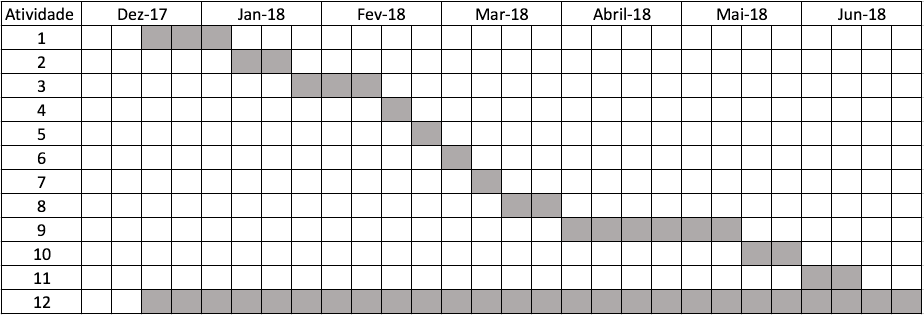
\includegraphics[scale=0.45]{./Figuras/cronograma.png}
  \end{center}
\end{figure}

\begin{enumerate}
\item Implementar a interface das recomendações
\item Incorporar ferramentas para facilitar o cálculo da similaridade do perfil do usuário com os itens
\item Implementar os algoritmos de recomendação (tradicional e a proposta desse trabalho)
\item Melhorar a categorização (palavras-chave) dos materiais e Links de Apoio presentes no minicurso de algoritmos
\item Realizar testes para garantir a funcionalidade dos algoritmos de recomendação desenvolvidos
\item Produzir os intrumentos necessários para o experimento
\item Convidar alunos a participar do experimento
\item Realizar o experimento
\item Estudar e definir as técnicas de análise dos dados
\item Analisar os dados (resultados do experimento)
\item Escrever a dissertação
\end{enumerate}

  \chapter{Teste Piloto}\label{ape:teste-piloto}

Protocolo:
\begin{itemize}
  \item Primeira etapa:
  \begin{enumerate}
  \item Acessar a página do AdaptWeb: http://200.19.107.172/adaptweb/
  \item Logar com o usuário testepiloto1@udesc.br e senha testepiloto1
  \item Acessar  o link http://200.19.107.172/adaptweb/index.php?opcao=MinicursoAlgoritmos e realizar a matrícula na disciplina
  \item Acessar o ambiente de aula da disciplina pelo modo de navegação dado:
  \item Livre ou Tutorial
  \item Acessar 5 conceitos da disciplina
  \item Encontrar as recomendações
  \item Quantos recomendações você recebeu?
  \item Olhando pelo título e descrição dos links, eles parecem estar de acordo com os conceitos que você acessou?
  \item Acessar as recomendações
  \item Avaliar as recomendações
  \item Acessar mais 3 conceitos da disciplina e um material complementar (dica: use o mapa de navegação presente na parte superior da tela)
  \item Analisar as recomendações para perceber se algo mudou
  \item Pedir para o aplicador do teste piloto habilitar a avaliação da disciplina
  \item Realizar a avaliação da disciplina
  \item Ao final da avaliação, responder ao questionário de satisfação
  \end{enumerate}

  \item Segunda etapa (avise o aplicador do teste antes de iniciar essa etapa):
  \begin{enumerate}
  \item Deslogar do ambiente se ainda estiver logado
  \item Acessar o link http://200.19.107.172/adaptweb/index.php?opcao=MinicursoAlgoritmos para criar um usuário no ambiente e depois se matricular na disciplina
  \item Verificar como está o acesso à disciplina
  \end{enumerate}
\end{itemize}
  \chapter{Termo de Consentimento Livre e Esclarecido}\label{ape:termo-de-consentimento}

\section{Descrição do Minicurso}

Você está sendo convidado a participar do Minicurso de Algoritmos vinculado a um projeto de mestrado. Este projeto intitula-se “Sistema de Recomendação Sensível ao Tempo em Ambientes Virtuais de Aprendizagem” e visa descobrir se o uso da informação temporal em um Sistema de Recomendação influencia na qualidade dos itens recomendados.
Durante o minicurso, seus dados de utilização serão coletados e posteriormente analisados pelos pesquisadores envolvidos no projeto.

\section{Procedimento}
Após o período de matrícula (de 09/04/2018 a 13/04/2018) no minicurso, todos os alunos matriculados terão acesso ao conteúdo do minicurso a partir do dia 16/04/2018. Ao final do minicurso, os alunos realizarão uma avaliação final e responderão a um questionário de satisfação referente ao minicurso.
Durante o minicurso, os dados de navegação/interação dos alunos com o AdaptWeb® serão coletados para análise posterior com o objetivo de descobrir aspectos positivos e negativos das ferramentas existentes no sistema.

\section{Riscos e Desconfortos}
A participação neste minicurso não apresenta riscos diretos a seus participantes. Caso você não se sinta confortável em ter suas informações coletadas; não goste do assunto abordado, da metodologia utilizada ou do material utilizado; ou ainda por quaisquer outros motivos não deseje continuar a participar do minicurso, você está livre pra desistir a qualquer momento.

\section{Benefícios da sua Participação}
Esperamos que os resultados obtidos auxiliem a identificar os benefícios práticos do uso da informação temporal em um Sistema de Recomendação através das recomendações realizadas para os alunos durante sua interação, suas características positivas e negativas. Desta forma, esperamos contribuir com uma melhor experiência do usuário em ambientes de Educação a Distância.


\section{Custos}
Sua participação no minicurso não acarretará em nenhum custo. Você também não será pago(a) para participar.

\section{Confidencialidade}
Sua identidade será preservada, pois você será referenciado por um identificador numérico, de forma que seu nome nunca será citado. As únicas pessoas que terão acesso aos dados brutos serão as pesquisadoras envolvidas no projeto: Eduardo José de Borba, profa. Dra. Isabela Gasparini e prof. Dr. Daniel Lichtnow. Os resultados, sem identificações, poderão ser veiculados em artigos técnicos e científicos.

\section{Dúvidas}
Caso haja qualquer dúvida a respeito do minicurso, sinta-se à vontade para entrar em contato.

\begin{quote}
\textbf{Eduardo José de Borba} (Aluno do Programa de Pós-Graduação em Computação Aplicada da Universidade do Estado de Santa Catarina)\\
E-mail: eduardojoseborba@gmail.com\\
\\
\textbf{Dra. Isabela Gasparini} (Orientadora)\\
E-mail: isabela.gasparini@udesc.br\\
\\
\textbf{Dr. Daniel Lichtnow} (Coorientador)\\
E-mail: dlichtnow@politecnico.ufsm.br\\
\\
\textbf{Endereço para contato:}\\
Departamento de Ciência da Computação (DCC)\\
Centro de Ciências Tecnológicas (CCT)\\
Rua Paulo Malschitzki, 200 - Campus Universitário Prof. Avelino Marcante - Bairro Zona Industrial Norte\\
Joinville - SC - Brasil\\
\end{quote}


\centerline{\textbf{Termo de Consentimento Livre e Esclarecido}}

Solicitamos a sua permissão para utilizarmos os dados coletados, bem como para divulgar os resultados em artigos técnicos e científicos. Lembramos que iremos garantir sua privacidade.
Destacamos que este estudo visa avaliar a ferramenta e não os participantes. Nós queremos saber a sua opinião!

\begin{todolist}
\item Declaro que fui informado sobre todos os procedimentos da pesquisa e, que recebi de forma clara e objetiva todas as explicações pertinentes ao projeto e, que todos os dados coletados serão sigilosos. Eu compreendo que neste estudo, as medições dos experimentos/procedimentos de tratamento serão feitas sobre minhas ações no sistema.
\item Declaro que meu responsável está ciente que estou participando deste minicurso, que dados sobre mim estão sendo coletados e que minha identidade será preservada.
\end{todolist}

Nome do responsável:

E-mail para contato:



  \chapter{Questionário de Satisfação - Questões selecionadas traduzidas}\label{ape:questionario-de-satisfacao}

\section{QUALITY OF RECOMMENDED ITEMS}
\subsection{Accuracy}
\begin{itemize}
\item \textbf{Questão 1:} Os itens recomendados corresponderam com os meus interesses.
\end{itemize}
\subsection{Diversity}
\begin{itemize}
\item \textbf{Questão 2:} Os itens recomendados para mim são diversificados (o sistema se preocupa em trazer itens diferentes a cada recomendação).
\end{itemize}
\subsection{Context Compatibility}
\begin{itemize}
\item \textbf{Questão 3:} Os itens recomendados corresponderam aos  interesses e necessidades que eu tinha no momento.
\item \textbf{Questão 4:} As recomendações são feitas no momento adequado.
\end{itemize}
\section{INTERACTION ADEQUACY}
\begin{itemize}
\item \textbf{Questão 5:} O sistema de recomendação explica porque os links são recomendados para mim.
\end{itemize}
\section{INTERFACE ADEQUACY}
\begin{itemize}
\item \textbf{Questão 6:} A informação apresentada na interface para os itens recomendados é suficiente para mim.
\item \textbf{Questão 7:} O layout do sistema de recomendação é atrativo e adequado.
\end{itemize}
\section{PERCEIVED EASE OF USE}
\subsection{Ease of Initial Learning}
\begin{itemize}
\item \textbf{Questão 8:} Eu encontrei facilmente o local onde os itens são recomendados.
\end{itemize}
\subsection{Ease of Preference Revision}
\begin{itemize}
\item \textbf{Questão 9:} Eu percebi que o sistema de recomendação aprendia sobre minhas necessidades/preferências conforme eu avançava na disciplina.
\end{itemize}
\subsection{Ease of Decision Making}
\begin{itemize}
\item \textbf{Questão 10:} É facil encontrar um item para estudar com a ajuda do sistema de recomendação.
\end{itemize}
\section{PERCEIVED USEFULNESS}
\begin{itemize}
\item \textbf{Questão 11:} Eu me senti apoiado para encontrar itens do meu interesse com a ajuda do sistema de recomendação.
\end{itemize}
\section{CONTROL/TRANSPARENCY}
\begin{itemize}
\item \textbf{Questão 12:} Eu entendi porque os itens foram recomendados para mim.
\end{itemize}
\section{ATTITUDES}
\begin{itemize}
\item \textbf{Questão 13:} No geral, estou satisfeito com o sistema de recomendação.
\end{itemize}

  \chapter{Dicionário de Palavras-chave}\label{ape:dicionario-palavras-chave}

\begin{longtable}{| p{.20\textwidth} | p{.80\textwidth} |}
\hline
\# & Palavras-chave            \\ \hline
1  & Algoritmo                 \\ \hline
2  & Aplicacao de algoritmo    \\ \hline
3  & Atribuicao                \\ \hline
4  & Blocos                    \\ \hline
5  & Comentario                \\ \hline
6  & Compilador                \\ \hline
7  & Constantes                \\ \hline
8  & Decisao composta          \\ \hline
9  & Decisao encadeada         \\ \hline
10 & Decisao simples           \\ \hline
11 & Diagrama de Chapin        \\ \hline
12 & Enquanto                  \\ \hline
13 & Entrada                   \\ \hline
14 & Escolha                   \\ \hline
15 & Estrutura condicional     \\ \hline
16 & Estrutura de repeticao    \\ \hline
17 & Estrutura sequencial      \\ \hline
18 & Fluxograma                \\ \hline
19 & Instrucao                 \\ \hline
20 & Interpretador             \\ \hline
21 & Linguagem C               \\ \hline
22 & Linguagem de maquina      \\ \hline
23 & Linguagem de programacao  \\ \hline
24 & Linguagem natural         \\ \hline
25 & Logica de programacao     \\ \hline
26 & Matriz                    \\ \hline
27 & Narrativa                 \\ \hline
28 & Operadores                \\ \hline
29 & Operadores aritmeticos    \\ \hline
30 & Operadores logicos        \\ \hline
31 & Operadores relacionais    \\ \hline
32 & Para                      \\ \hline
33 & Portugol                  \\ \hline
34 & Precedencia de operadores \\ \hline
35 & Problema                  \\ \hline
36 & Processamento             \\ \hline
37 & Programa de computador    \\ \hline
38 & Pseudocodigo              \\ \hline
39 & Repita                    \\ \hline
40 & Saida                     \\ \hline
41 & Se                        \\ \hline
42 & Semantica                 \\ \hline
43 & Sintaxe                   \\ \hline
44 & Tipo caracter             \\ \hline
45 & Tipo inteiro              \\ \hline
46 & Tipo logico               \\ \hline
47 & Tipo real                 \\ \hline
48 & Tipo texto                \\ \hline
49 & Tipos de algoritmo        \\ \hline
50 & Tipos de dados            \\ \hline
51 & Variaveis                 \\ \hline
52 & Vetor                     \\ \hline
\caption{Dicionário de Palavras-chave}
\label{tab:dicionario-palavras-chave}
\end{longtable}
  \chapter{Palavras-chave dos materiais no Minicurso de Algotimos e Linguagem de Programação}\label{ape:dicionario-palavras-chave}

\section{Links de Apoio}

\begin{longtable}{| p{.10\textwidth} | p{.45\textwidth} | p{.45\textwidth} |}
\hline
\#  & Link de Apoio                                                                                                                                                                                                                & palavras\_chave                                                                                                                                   \\ \hline
1   & \href{http://academicotech.blogspot.com.br/2014/02/v-behaviorurldefaultvmlo.html}{Lógica de Programação - Fluxograma e Portugol                                       } & Logica de programacao, Fluxograma, Portugol, Pseudocodigo, Operadores, Blocos, Tipos de dados, Variaveis,                                         \\ \hline
2   & \href{http://blog.academiadocodigo.com.br/2014/12/macas-e-laranjas-diferencas-entre-compilador-e-interpretator/}{Maçãs e laranjas: diferenças entre compilador e interpretator                       } & Compilador, Interpretador                                                                                                                         \\ \hline
3   & \href{http://blog.triadworks.com.br/por-que-aprender-a-programar}{Por que aprender a programar?                                                       } & Aplicacao de algoritmo, Programa de computador                                                                                                    \\ \hline
4   & \href{http://br.ccm.net/faq/9709-algoritmo-definicao-e-introducao}{Algoritmo: Definição e introdução                                                   } & Algoritmo, Linguagem de maquina, Compilador, Linguagem de programacao                                                                             \\ \hline
5   & \href{http://coral.ufsm.br/pet-si/index.php/os-beneficios-e-o-porque-de-aprender-a-programar/}{Os Benefícios e o Porquê de Aprender a Programar.                                   } & Aplicacao de algoritmo, Algoritmo, Instrucao, Programa de computador                                                                              \\ \hline
6   & \href{http://dcm.ffclrp.usp.br/~augusto/teaching/ici/Vetores-Matrizes.pdf}{Vetores e Matrizes                                                                  } & Vetor, Matriz, Contantes, Entrada, Saida                                                                                                          \\ \hline
7   & \href{http://download2.nust.na/pub4/sourceforge/v/vi/visualg30/IP\_03\_VisuALG\_Repeticao.pdf}{VisuALG - estrutura de repetição                                                    } & Estrutura de repetição, Enquanto, Para, Repita                                                                                                    \\ \hline
8   & \href{http://download2.nust.na/pub4/sourceforge/v/vi/visualg30/IP\_02\_VisuALG\_Basico.pdf}{Introdução ao VisuALG                                                               } & Portugol, Entrada, Saida, Operadores aritmeticos, Precedencia de operadores, Operadores logicos, Estrutura condicional                            \\ \hline
9   & \href{http://download2.nust.na/pub4/sourceforge/v/vi/visualg30/IP\_04\_VisuALG\_Arrays.pdf}{VisuALG – Arrays e Strings                                                          } & Portugol, Vetor, Tipo texto                                                                                                                       \\ \hline
10  & \href{http://eletrica.ufpr.br/~rogerio/visualg/Help/linguagem.htm}{A Linguagem de Programação do VisuAlg                                               } & Portugol, Pseudocodigo, Tipos de dados, Variaveis, Constantes                                                                                     \\ \hline
11  & \href{http://fabrica.ms.senac.br/2013/06/algoritmo-estrutura-de-vetores-e-matrizes/}{Algoritmo: Estrutura de vetores e matrizes.                                         } & Portugol, Entrada, Saida, Vetor, Matriz                                                                                                           \\ \hline
12  & \href{http://fig.if.usp.br/~esdobay/c/c.pdf}{Programação em C                                                                    } & Linguagem C, Variaveis, Constantes, Operadores, Vetor, Matriz                                                                                     \\ \hline
13  & \href{http://knoow.net/ciencinformtelec/informatica/linguagem-maquina/}{Linguagem máquina                                                                   } & Linguagem de maquina                                                                                                                              \\ \hline
14  & \href{http://linguagemc.com.br/estruturas-de-decisao-encadeadas-if-else-if-else/}{Estruturas de decisão encadeadas – if – else – if – else                            } & Estrutura condicional, Decisao Encadeada, Se                                                                                                      \\ \hline
15  & \href{http://linguagemc.com.br/loop-infinito-em-c/}{Loop infinito em C                                                                  } & Linguagem C, Estrutura de repeticao, Para, Repita                                                                                                 \\ \hline
16  & \href{http://marmsx.msxall.com/cursos/c3.html}{Começando a programar                                                               } & Linguagem C, Sintaxe, Semantica                                                                                                                   \\ \hline
17  & \href{http://nerdsti.com.br/?p=259}{Lógica de Programação - Vetores e Matrizes                                          } & Vetor, Matriz, Sintaxe                                                                                                                            \\ \hline
18  & \href{http://wiki.icmc.usp.br/images/5/57/Estruturas\_Controle\_I\_SCC0120\_v2.pdf}{Introdução à Ciência da Computação - Estruturas de Controle – Parte I               } & Portugol, Estrutura condicional, Decisao simples, Decisao composta, Decisao encadeada                                                             \\ \hline
19  & \href{http://www.berriel.com.br/ltpi/aula01/aula01.htm}{Conceito e formas de representação de algoritmos                                    } & Algoritmo, Tipos de algoritmo, Narrativa, Fluxograma, Pseudocodigo                                                                                \\ \hline
20  & \href{http://www.bosontreinamentos.com.br/logica-de-programacao/12-logica-de-programacao-desvio-condicional-aninhado-se-entao-senao-se/}{Lógica de Programação – Desvio Condicional Aninhado (SE…ENTÃO…SENÃO…SE)             } & Portugol, Estrutura condicional, Decisao composta, Se                                                                                             \\ \hline
21  & \href{http://www.cprogressivo.net/2013/03/O-que-e-alocacao-dinamica-de-memoria-em-Linguagem-C.html}{O que é e para que serve alocação dinâmica                                          } & Linguagem C, Vetor                                                                                                                                \\ \hline
22  & \href{http://www.cprogressivo.net/p/arquivos-em-c.html}{Arquivos em c - tutorial completo                                                   } & Linguagem C                                                                                                                                       \\ \hline
23  & \href{http://www.cristiancechinel.pro.br/my\_files/algorithms/bookhtml/node18.html}{Linguagem Natural                                                                   } & Linguagem natural                                                                                                                                 \\ \hline
24  & \href{http://www.cristiancechinel.pro.br/my\_files/algorithms/bookhtml/node19.html}{Linguagem de Máquina e Assembler                                                    } & Linguagem de maquina                                                                                                                              \\ \hline
25  & \href{http://www.cristiancechinel.pro.br/my\_files/algorithms/bookhtml/node43.html}{Expressões Lógicas                                                                  } & Operadores logicos                                                                                                                                \\ \hline
26  & \href{http://www.cristiancechinel.pro.br/my\_files/algorithms/bookhtml/node44.html}{Operadores Relacionais                                                              } & Operadores relacionais                                                                                                                            \\ \hline
27  & \href{http://www.dainf.cefetpr.br/~robson/prof/common/c/aspec.htm}{Aspectos básicos de linguagem C                                                     } & Linguagem C, Tipos de dados, Variaveis, Constantes, Entrada, Saida, Operadores                                                                    \\ \hline
28  & \href{http://www.dei.estt.ipt.pt/portugol/node/10}{Tipos de dados \textgreater{}\textgreater Constantes                                } & Constantes, Portugol                                                                                                                              \\ \hline
29  & \href{http://www.dei.estt.ipt.pt/portugol/node/14}{Entrada/Saída \textgreater{}\textgreater Ler                                        } & Entrada, Portugol                                                                                                                                 \\ \hline
30  & \href{http://www.dei.estt.ipt.pt/portugol/node/15}{Entrada/Saída \textgreater{}\textgreater Escrever                                   } & Saida, Portugol                                                                                                                                   \\ \hline
31  & \href{http://www.dei.estt.ipt.pt/portugol/node/17}{Operadores Aritméticos                                                              } & Operadores aritmeticos, Portugol                                                                                                                  \\ \hline
32  & \href{http://www.dei.estt.ipt.pt/portugol/node/21}{Operadores Lógicos                                                                  } & Operadores logicos, Portugol                                                                                                                      \\ \hline
33  & \href{http://www.dei.estt.ipt.pt/portugol/node/22}{Operadores Relacionais                                                              } & Operadores relacionais, Portugol                                                                                                                  \\ \hline
34  & \href{http://www.dei.estt.ipt.pt/portugol/node/24}{Decisão \textgreater{}\textgreater Se                                               } & Se, Estrutura condicional, Portugol                                                                                                               \\ \hline
35  & \href{http://www.dei.estt.ipt.pt/portugol/node/25}{Decisão \textgreater{}\textgreater Escolhe                                          } & Escolha, Estrutura condicional, Portugol                                                                                                          \\ \hline
36  & \href{http://www.dei.estt.ipt.pt/portugol/node/27}{Repetição \textgreater{}\textgreater Enquanto                                       } & Enquanto, Estrutura de repeticao, Portugol                                                                                                        \\ \hline
37  & \href{http://www.dei.estt.ipt.pt/portugol/node/28}{Repetição \textgreater{}\textgreater Para                                           } & Para, Estrutura de repeticao, Portugol                                                                                                            \\ \hline
38  & \href{http://www.dei.estt.ipt.pt/portugol/node/29}{Repetição \textgreater{}\textgreater Repete                                         } & Repita, Estrutura de repeticao, Portugol                                                                                                          \\ \hline
39  & \href{http://www.dei.estt.ipt.pt/portugol/node/30}{Repetição \textgreater{}\textgreater Faz                                            } & Repita, Estrutura de repeticao, Portugol                                                                                                          \\ \hline
40  & \href{http://www.dei.estt.ipt.pt/portugol/node/6}{Linguagem Algorítmica                                                               } & Sintaxe, Semantica, Portugol                                                                                                                      \\ \hline
41  & \href{http://www.dei.estt.ipt.pt/portugol/node/8}{Tipos de dados \textgreater{}\textgreater Básicos                                   } & Tipos de dados, Tipo inteiro, Tipo real, Tipo logico, Tipo caracter, Tipo texto                                                                   \\ \hline
42  & \href{http://www.dei.estt.ipt.pt/portugol/node/9}{Tipos de dados \textgreater{}\textgreater Variáveis                                 } & Variaveis, Portugol                                                                                                                               \\ \hline
43  & \href{http://www.devmedia.com.br/fluxogramas-diagrama-de-blocos-e-de-chapin-no-desenvolvimento-de-algoritmos/28550}{Fluxogramas, diagrama de blocos e de Chapin no desenvolvimento de algoritmos        } & Tipos de algoritmo, Fluxograma                                                                                                                    \\ \hline
44  & \href{http://www.dicasdeprogramacao.com.br/estrutura-de-selecao-multipla-escolha-caso/}{Estrutura de seleção multipla ESCOLHA-CASO                                          } & Estrutura condicional, Decisao encadeada, Escolha                                                                                                 \\ \hline
45  & \href{http://www.dicasdeprogramacao.com.br/o-que-e-algoritmo/}{O que é Algoritmo?                                                                  } & Algoritmo, Problema                                                                                                                               \\ \hline
46  & \href{http://www.din.uem.br/~teclopes/FCaula5.pdf}{Algoritmos – Estruturas de Controle                                                 } & Estrutura condicional, Decisao simples, Decisao composta, Decisao encadeada, Se, Escolha                                                          \\ \hline
47  & \href{http://www.gazetadopovo.com.br/vida-e-cidadania/o-uso-cotidiano-do-algoritmo-4x3n9sw4bkhoam6fzqcp27mfi}{O uso cotidiano do algoritmo                                                        } & Aplicacao de algoritmo                                                                                                                            \\ \hline
48  & \href{http://www.ic.unicamp.br/~sheila/mc102/02\_Entrada\%20Saida\%20e\%20Operadores.pdf}{Comandos de entrada e saída                                                         } & Linguagem C, Entrada, Saida, Atribuicao, Operadores                                                                                               \\ \hline
49  & \href{http://www.ic.unicamp.br/~wainer/cursos/2s2011/Cap05-EstruturasCondicionais-texto.pdf}{Estruturas Condicionais                                                             } & Linguagem C, Estrutura condicional, Operadores relacionais                                                                                        \\ \hline
50  & \href{http://www.inf.pucrs.br/~benso/progi/guia.htm}{Programação para Engenharia I                                                       } & Linguagem C, Tipos de dados, Tipo texto                                                                                                           \\ \hline
51  & \href{http://www.inf.pucrs.br/~pinho/LaproI/ComandosDeRepeticao/Repeticao.html}{Comandos de decisão Comandos de seleção                                             } & Linguagem C, Estrutura condicional, Estrutura de repeticao                                                                                        \\ \hline
52  & \href{http://www.inf.pucrs.br/~pinho/LaproI/IntroC/IntroC.htm}{Introdução à Linguagem C                                                            } & Variaveis, Tipos de dados, Tipo texto, Entrada, Saida, Tipo real, Operadores aritmeticos                                                          \\ \hline
53  & \href{http://www.inf.pucrs.br/~pinho/LaproI/Vetores/Vetores.htm}{Matrizes e Vetores                                                                  } & Linguagem C, Vetor, Matriz, Entrada, Saida, Atribuicao                                                                                            \\ \hline
54  & \href{http://www.inf.ufpr.br/cursos/ci067/Docs/NotasAula/notas-19\_Arrays\_Multidimensionais.html}{Arrays multidimensionais                                                            } & Vetor, Matriz                                                                                                                                     \\ \hline
55  & \href{http://www.inf.ufpr.br/cursos/ci067/Docs/NotasAula/notas-6\_Operadores\_Logicos.html}{Operadores Lógicos                                                                  } & Linguagem C, Operadores logicos                                                                                                                   \\ \hline
56  & \href{http://www.inf.ufsc.br/~bosco/ensino/ine5201/ApostilaVisuAlg20.pdf}{Manual do Visualg                                                                   } & Portugol, Variaveis, Tipos de dados, Sintaxe, Constantes, Atribuicao, Entrada, Saida, Operadores, Estrutura condicional, Estrutura de repeticao   \\ \hline
57  & \href{http://www.ipb.pt/~cmca/algor1.pdf}{Noção e Representação de Algoritmos                                                 } & Algoritmo, Tipos de algoritmo, Problema, Narrativa, Fluxograma                                                                                    \\ \hline
58  & \href{http://www.omundodaprogramacao.com/representacao-de-algoritmos/}{Representação de Algoritmos                                                         } & Algoritmo, Tipos de algoritmo, Narrativa, Fluxograma, Diagrama de Chapin, Pseudocodigo                                                            \\ \hline
59  & \href{http://www.rafaeltoledo.net/estruturas-de-selecao/}{Estrutura de seleção                                                                } & Pseudocodigo, Estrutura condicional                                                                                                               \\ \hline
60  & \href{http://www.rafaeltoledo.net/introducao-a-linguagem-c-parte-i/}{Introdução à linguagem C - Parte 1                                                  } & Linguagem C, Tipos de dados, Operadores relacionais, Tipo texto                                                                                   \\ \hline
61  & \href{http://www.rafaeltoledo.net/introducao-a-logica-de-programacao/}{Introdução à lógica de programação                                                  } & Algoritmo, Logica de programacao, Portugol, Pseudolinguagem                                                                                       \\ \hline
62  & \href{http://www.rafaeltoledo.net/lacos-de-repeticao/}{Laços de repetição                                                                  } & Pseudocodigo, Estrutura de repeticao                                                                                                              \\ \hline
63  & \href{http://www.rafaeltoledo.net/vetores-e-matrizes/}{Vetores e Matrizes                                                                  } & Pseudocodigo, Vetor, Matriz                                                                                                                       \\ \hline
64  & \href{http://www.tecmundo.com.br/programacao/2082-o-que-e-algoritmo-.htm}{O que é algoritmo?                                                                  } & Algoritmo, Tipos de algoritmo                                                                                                                     \\ \hline
65  & \href{http://www.tiexpert.net/programacao/algoritmo/o-que-e-um-algoritmo.php}{O que é um algoritmo?                                                               } & Algoritmo                                                                                                                                         \\ \hline
66  & \href{http://www.univasf.edu.br/~andreza.leite/aulas/AP/VetoresMatrizes.pdf}{Vetores e Matrizes                                                                  } & Vetor, Matriz                                                                                                                                     \\ \hline
67  & \href{http://www.univasf.edu.br/~jose.valentim/aula1.pdf}{Algoritmo e Programação                                                             } & Algoritmo, Tipos de algoritmo, Fluxograma, Narrativa, Portugol, Variaveis, Tipos de dados                                                         \\ \hline
68  & \href{http://www.univasf.edu.br/~ricardo.aramos/disciplinas/AlgProgAgr\_2011\_1/cap03AnaEmilia.pdf}{Estruturas de Controle                                                              } & Estrutura sequencial, Estrutura condicional, Decisao simples, Decisao composta, Decisao encadeada, Estrutura de repeticao, Para, Repita, Enquanto \\ \hline
69  & \href{https://becode.com.br/principais-linguagens-de-programacao/}{As 15 principais linguagens de programação do mundo!                                } & Linguagem de programacao                                                                                                                          \\ \hline
70  & \href{https://dicasdeprogramacao.com.br/o-que-sao-vetores-e-matrizes-arrays/}{O que são Vetores e Matrizes (arrays)                                               } & Vetor, Matriz, Portugol, Estrutura de repeticao                                                                                                   \\ \hline
71  & \href{https://dicasdeprogramacao.com.br/operadores-relacionais/}{Conheça os Operadores Relacionais!                                                  } & Portugol, Operadores relacionais                                                                                                                  \\ \hline
72  & \href{https://lucianopascal.wordpress.com/2010/04/02/aprendendo-a-interpretar-exercicios-de-algoritmos/}{Aprendendo a interpretar exercícios de algoritmos                                   } & Algoritmo, Problema, Entrada, Processamento, Saida                                                                                                \\ \hline
73  & \href{https://msdn.microsoft.com/pt-br/library/474dd6e2.aspx}{Operadores de atribuição C                                                          } & Linguagem C, Atribuicao                                                                                                                           \\ \hline
74  & \href{https://msdn.microsoft.com/pt-br/library/6swh93dx.aspx}{Operadores relacionais e de igualdade C                                             } & Linguagem C, Operadores relacionais                                                                                                               \\ \hline
75  & \href{https://msdn.microsoft.com/pt-br/library/exefbdtf.aspx}{Operador de expressão condicional                                                   } & Linguagem C, Operadores logicos, Operadores relacionais, Estrutura condicional                                                                    \\ \hline
76  & \href{https://msdn.microsoft.com/pt-br/library/z68fx2f1.aspx}{Operadores lógicos C                                                                } & Linguagem C, Operadores logicos                                                                                                                   \\ \hline
77  & \href{https://pt.wikipedia.org/wiki/Algoritmo}{Algoritmo                                                                           } & Algoritmo, Tipos de algoritmo, Programa de computador, Interpretador, Compilador                                                                  \\ \hline
78  & \href{https://pt.wikipedia.org/wiki/Estrutura\_de\_controle}{Estrutura de controle                                                               } & Estrutura sequencial, Estrutura condicional, Estrutura de repeticao                                                                               \\ \hline
79  & \href{https://pt.wikipedia.org/wiki/Estrutura\_de\_repeti\%C3\%A7\%C3\%A3o}{Estrutura de repetição                                                              } & Estrutura de repeticao, Enquanto, Para, Repita                                                                                                    \\ \hline
80  & \href{https://pt.wikipedia.org/wiki/Operadores\_em\_C\_e\_C\%2B\%2B}{Operadores em C e C++                                                               } & Linguagem C, Operadores                                                                                                                           \\ \hline
81  & \href{https://sites.google.com/site/itabits/treinamento/introducao-a-programacao-em-c/comandos-de-repeticao}{Comandos de Repetição (Laços ou Loops)                                              } & Linguagem C, Estrutura de repeticao, Enquanto, Para, Repita                                                                                       \\ \hline
82  & \href{https://www.dca.ufrn.br/~ivan/DCA0800/tiposDados.pdf}{Outros conceitos sobre logica de programação: Tipos de dados, variaveis e expressões} & Tipos de dados, Variaveis, Operacoes, Operacoes aritmeticas, Operacoes logicas                                                                    \\ \hline
83  & \href{https://www.dcc.fc.up.pt/~nam/aulas/9900/ic/slides/sliic9918/}{Linguagens de Programação                                                           } & Linguagem de programacao, Linguagem de maquina, Compilador                                                                                        \\ \hline
84  & \href{https://www.devmedia.com.br/estrutura-de-decisao-em-c-c/24031}{Estrutura de Decisão em C/C++                                                       } & Linguagem C, Estrutura condicional, Se, Escolha                                                                                                   \\ \hline
85  & \href{https://www.ime.usp.br/~hitoshi/introducao/03-Fundamentos.pdf}{Fundamentos                                                                         } & Linguagem C, Entrada, Saida, Atribuicao, Operadores, Variaveis, Precedencia de operadores                                                         \\ \hline
86  & \href{https://www.ime.usp.br/~pf/algoritmos/aulas/aloca.html}{Alocação dinâmica de memória                                                        } & Vetor, Matriz, Linguagem C                                                                                                                        \\ \hline
87  & \href{https://www.ime.usp.br/~pf/algoritmos/aulas/string.html}{Strings                                                                             } & Tipo texto, Entrada, Saida, Constantes                                                                                                            \\ \hline
88  & \href{https://www.inf.pucrs.br/~pinho/LaproI/Vetores/Vetores.htm}{Programação C/C++ - Matrizes e Vetores                                              } & Linguagem C, Vetor, Matriz                                                                                                                        \\ \hline
89  & \href{https://www.learnconline.com/2010/03/if-else-statement-c-programming-language.html}{The if-else Statement in c programming language                                     } & Se, Linguagem C                                                                                                                                   \\ \hline
90  & \href{https://www.learnconline.com/2010/03/while-loop-statement-in-c.html}{While Statement in c programming language                                           } & Enquanto, Linguagem C                                                                                                                             \\ \hline
91  & \href{https://www.programiz.com/c-programming/c-multi-dimensional-arrays}{C Programming Multidimensional Arrays                                               } & Linguagem C, Vetor, Matriz                                                                                                                        \\ \hline
92  & \href{https://www.tutorialspoint.com/cprogramming/c\_arrays.htm}{C- arrays                                                                           } & Linguagem C, Vetor                                                                                                                                \\ \hline
93  & \href{https://www.tutorialspoint.com/cprogramming/c\_multi\_dimensional\_arrays.htm}{Multi-dimensional Arrays in C                                                       } & Linguagem C, Matriz                                                                                                                               \\ \hline
94  & \href{https://www.tutorialspoint.com/cprogramming/c\_strings.htm}{C - Strings                                                                         } & Linguagem C, Tipo texto                                                                                                                           \\ \hline
95  & \href{https://www.youtube.com/watch?v=7oA8SBAOOAo}{Programar em C - Revisão Vetores/Matrizes                                           } & Vetor, Matriz, Problema                                                                                                                           \\ \hline
96  & \href{https://www.youtube.com/watch?v=7ph98Ih\_ckc}{Lógica de programação - Aula 03 - Legibilidade do código                            } & Algoritmo, Comentario, Blocos                                                                                                                     \\ \hline
97  & \href{https://www.youtube.com/watch?v=Ds1n6aHchRU}{Lógica de programação - Aula 01 - Introdução                                        } & Logica de programacao, Aplicacao de algoritmo                                                                                                     \\ \hline
98  & \href{https://www.youtube.com/watch?v=dZq7l9Oj-\_c}{Portugol - VisuALG - Aula 01 (Princípios Básicos)                                   } & Tipos de dados, Tipo inteiro, Tipo real, Tipo logico, Tipo caracter, Entrada, Saida, Atribuicao, Operadores aritmeticos                           \\ \hline
99  & \href{https://www.youtube.com/watch?v=ED7QtgXDShY}{Libraries                                                                           } & Linguagem C                                                                                                                                       \\ \hline
100 & \href{https://www.youtube.com/watch?v=g0iIVeeQo1M}{Lógica de programação - Aula 05 - Expressões, operadores e comandos                 } & Entrada, Saida, Operadores, Operadores relacionais, Operadores lógicos, Operadores aritmeticos, Atribuicao                                        \\ \hline
101 & \href{https://www.youtube.com/watch?v=JLlTo3SwxJE}{Lógica de programação - Aula 02 - Tipos de algoritmo                                } & Tipos de algoritmo, Fluxograma, Pseudocodigo, Narrativa                                                                                           \\ \hline
102 & \href{https://www.youtube.com/watch?v=l26oaHV7D40}{Programming Basics: Statements \& Functions: Crash Course Computer Science          } & Semantica, Sintaxe, Blocos                                                                                                                        \\ \hline
103 & \href{https://www.youtube.com/watch?v=Lelg\_sOYSm0}{Portugol Studio - Teste de Mesa                                                     } & Algoritmo, Processamento, Logica de programacao                                                                                                   \\ \hline
104 & \href{https://www.youtube.com/watch?v=mHW1Hsqlp6A}{Por que todos deveriam aprender a programar?                                        } & Aplicacao de algoritmo                                                                                                                            \\ \hline
105 & \href{https://www.youtube.com/watch?v=UuTmEcy5rV0}{Vetores e Matrizes                                                                  } & Vetor, Matriz, Fluxograma, Pseudocodigo                                                                                                           \\ \hline
106 & \href{https://www.youtube.com/watch?v=vgu8x\_Ivjd0}{Lógica de Programação - Estruturas de Repetição (Enquanto, Para, FacaEnquanto)      } & Logica de programacao, Estrutura de repeticao, Para, Enquanto, Repita                                                                             \\ \hline
107 & \href{https://www.youtube.com/watch?v=vp4jgXA\_BB0}{Lógica de programação - Aula 04 - Variáveis e constantes                            } & Variaveis, Constantes, Tipos de dados, Tipo inteiro, Tipo real, Tipo texto, Tipo logico, Vetor, Matriz                                            \\ \hline
108 & \href{https://www.zemoleza.com.br/trabalho-academico/exatas/informatica/as-principais-bibliotecas-em-linguagem-c/}{As principais bibliotecas em linguagem C                                            } & Linguagem C \\ \hline
\caption{Palavras-chave associadas com os Links de Apoio}
\label{tab:palavras-chave-links-de-apoio}
\end{longtable}

  \chapter{Intervenções}\label{ape:intervencoes}

No decorrer do minicurso, foram realizadas 12 intervenções por e-mail e pelo mural
de recados para estimular os alunos de ambos os grupos (i.e., os alunos que usaram o Sistema de Recomendação Tradicional
ou a proposta desse trabalho) a acessar o ambiente de aula e se aprofundar nos materiais instrucionais
liberados. Cada uma dessas intervenções e sua respectiva data é apresentada abaixo.

\begin{figure}[htb]
  \caption{\label{fig:intervencao-1}Intervenção 1 (16/04/18)}
  \begin{center}
      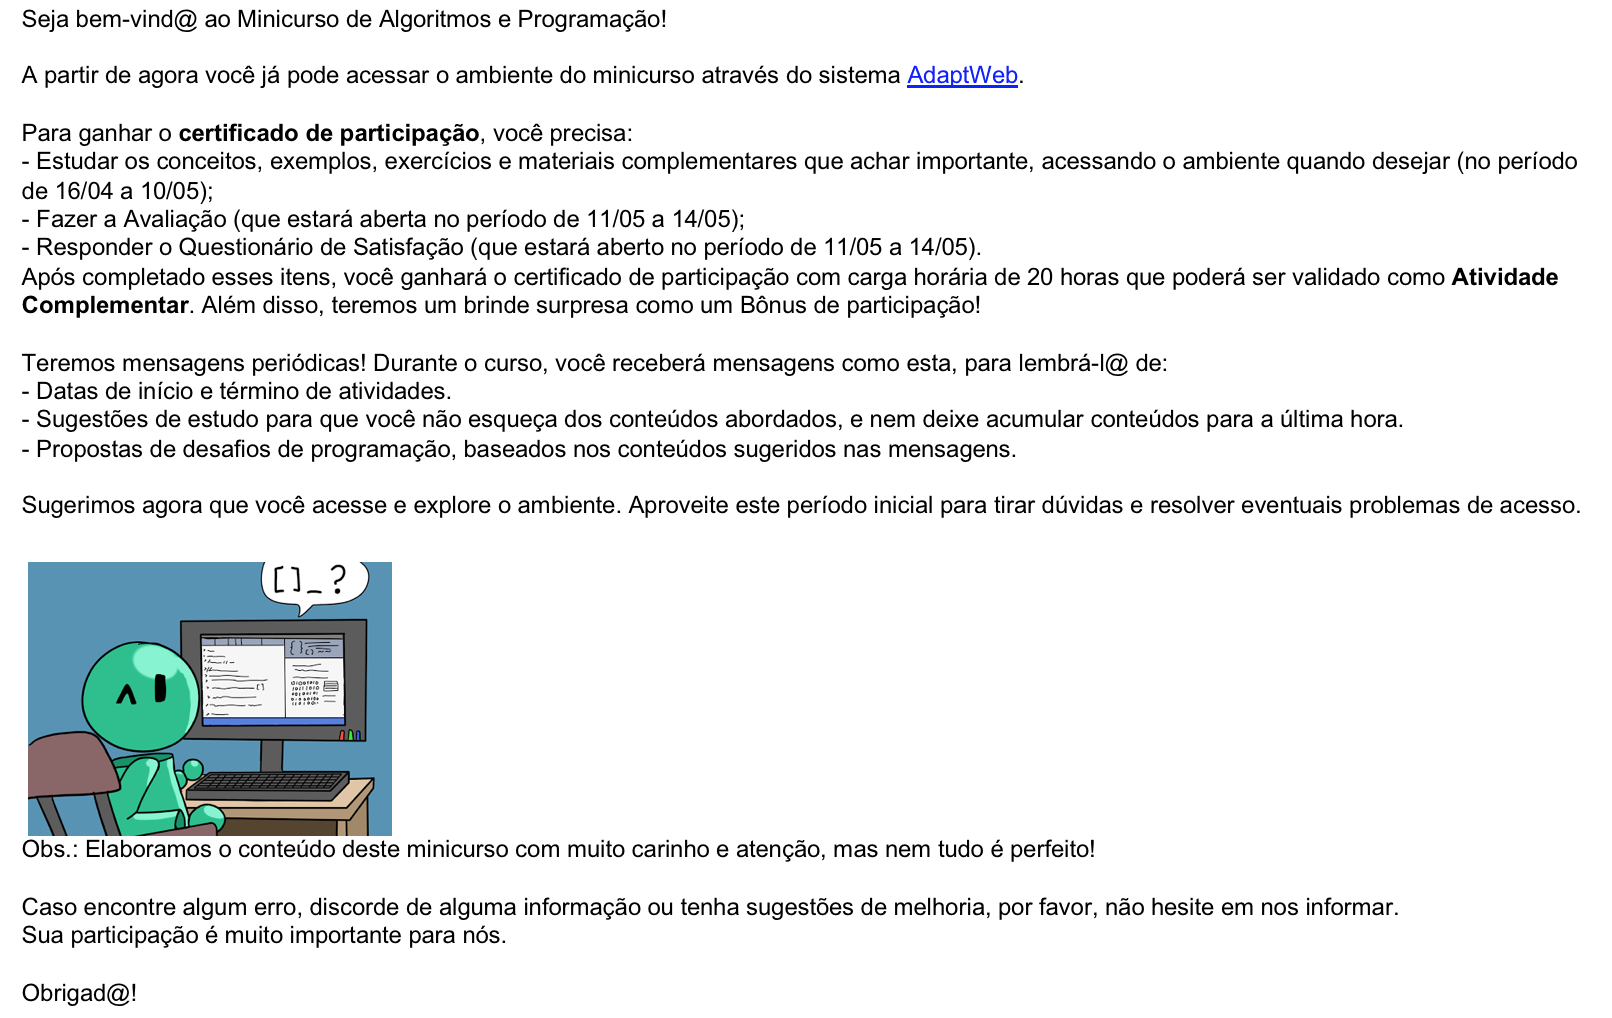
\includegraphics[scale=0.6]{./Figuras/intervencao-1.png}
  \end{center}
  \legend{Fonte: O autor.}
\end{figure}

\begin{figure}[htb]
  \caption{\label{fig:intervencao-2}Intervenção 2 (18/04/18)}
  \begin{center}
      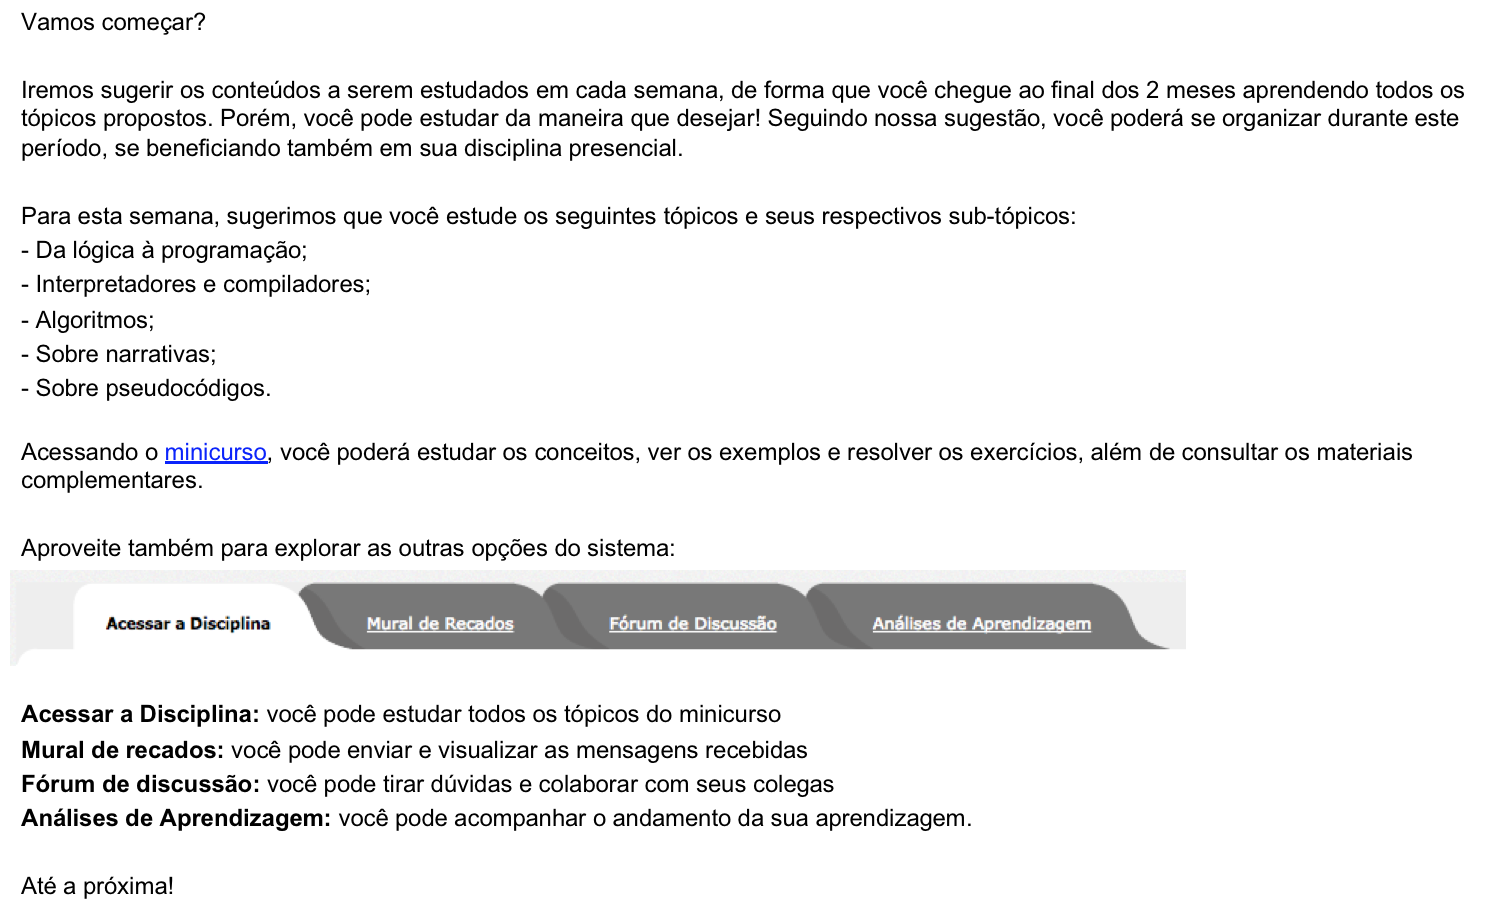
\includegraphics[scale=0.6]{./Figuras/intervencao-2.png}
  \end{center}
  \legend{Fonte: O autor.}
\end{figure}

\begin{figure}[htb]
  \caption{\label{fig:intervencao-3}Intervenção 3 (20/04/18)}
  \begin{center}
      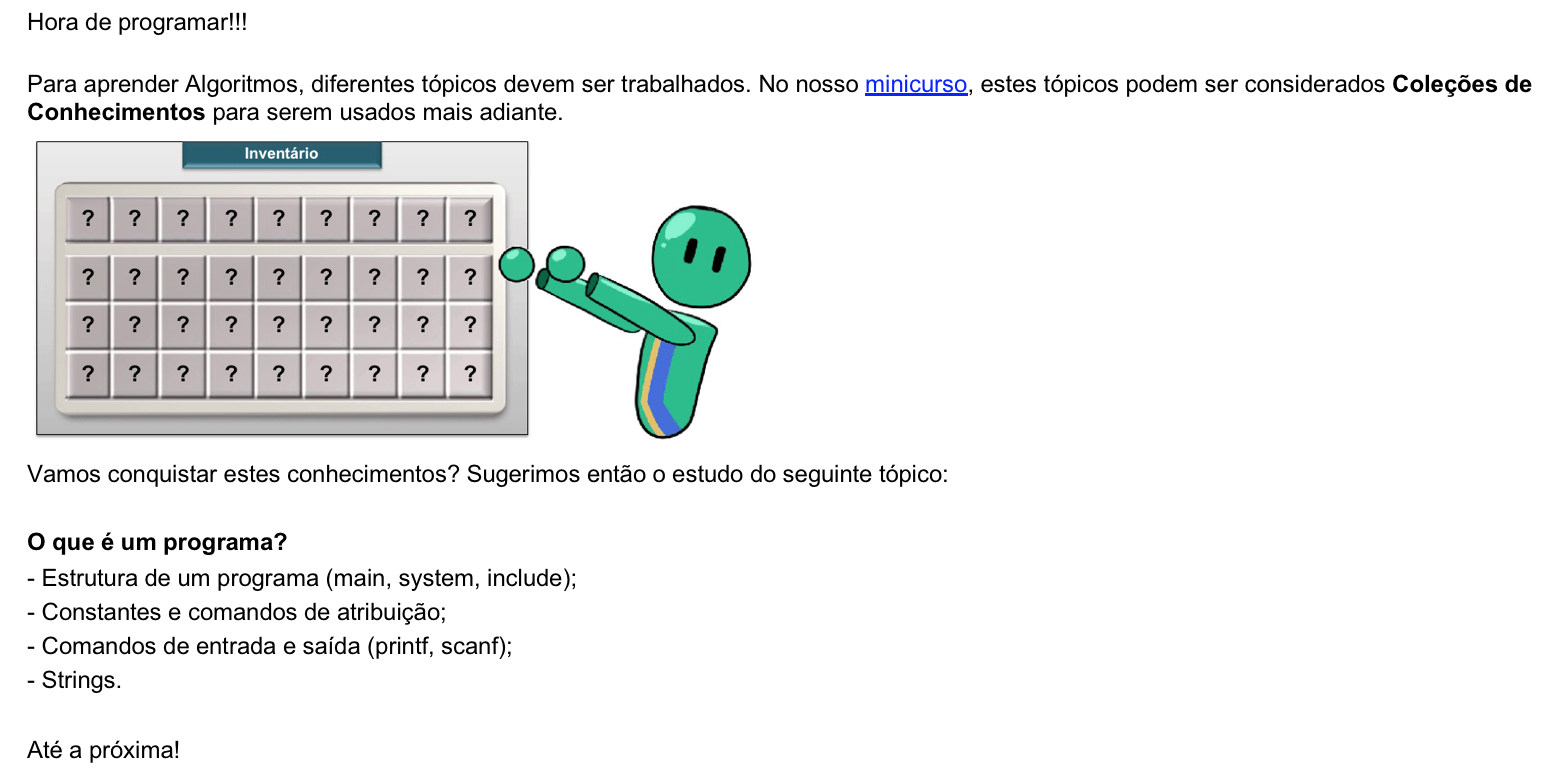
\includegraphics[scale=0.6]{./Figuras/intervencao-3.png}
  \end{center}
  \legend{Fonte: O autor.}
\end{figure}

\begin{figure}[htb]
  \caption{\label{fig:intervencao-4}Intervenção 4 (22/04/18)}
  \begin{center}
      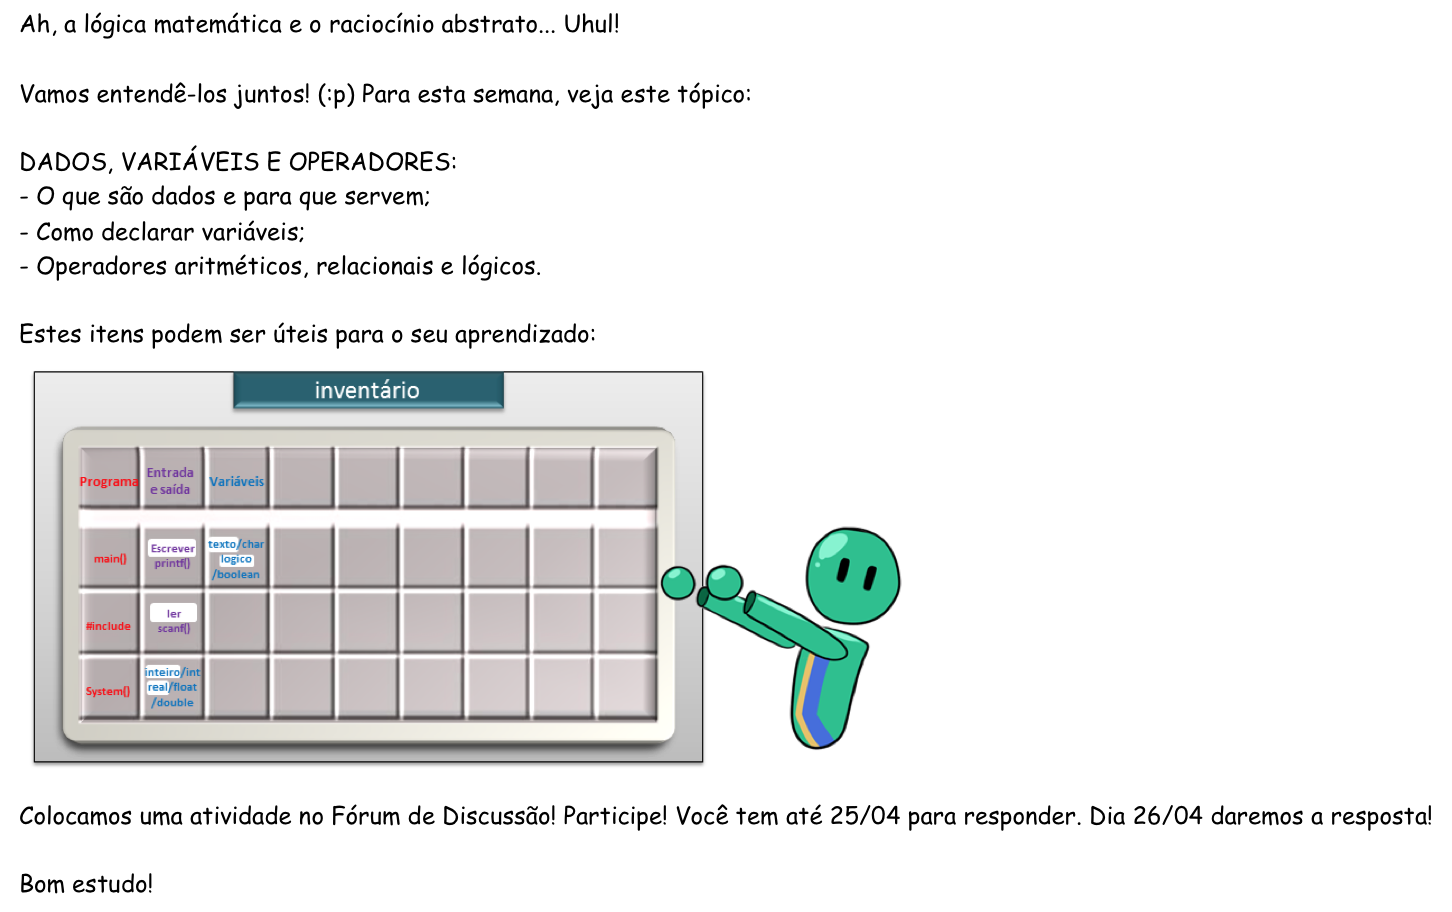
\includegraphics[scale=0.6]{./Figuras/intervencao-4.png}
  \end{center}
  \legend{Fonte: O autor.}
\end{figure}

\begin{figure}[htb]
  \caption{\label{fig:intervencao-5}Intervenção 5 (25/04/18)}
  \begin{center}
      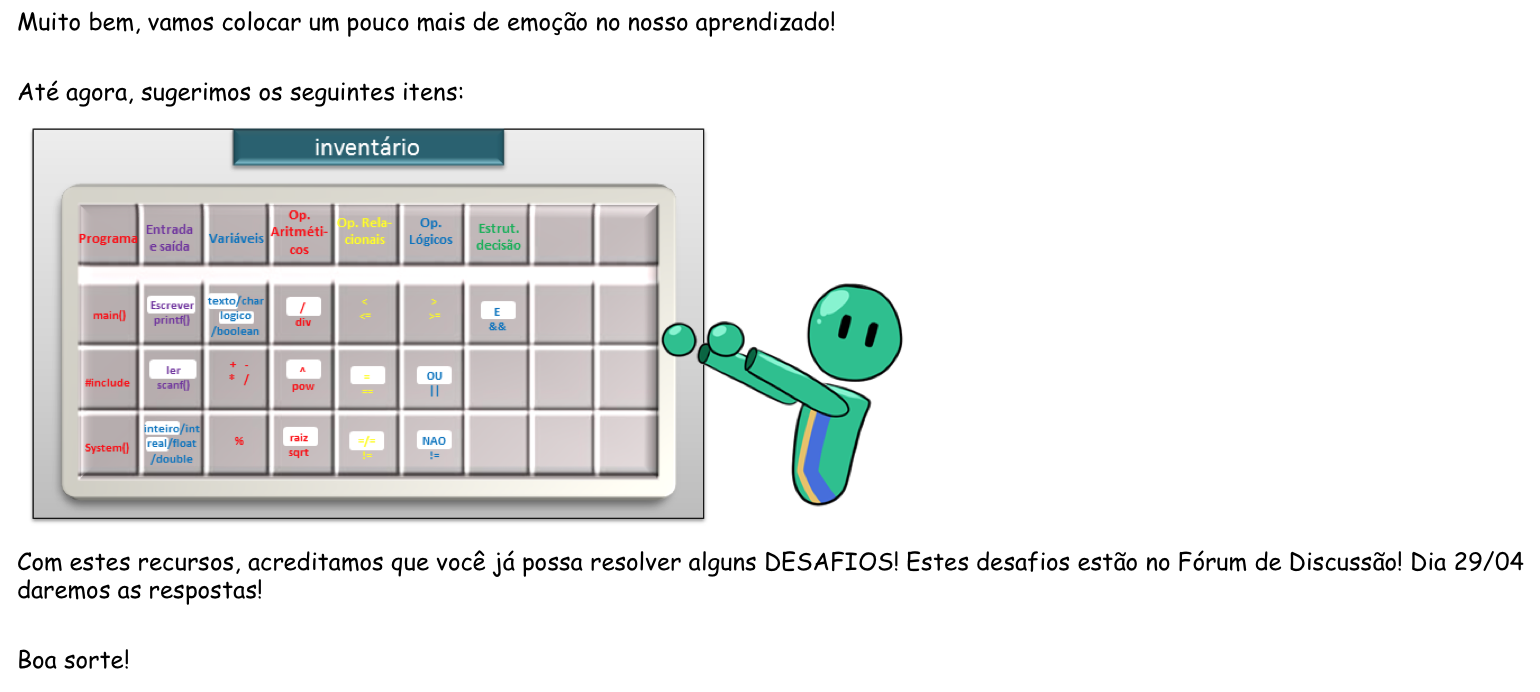
\includegraphics[scale=0.6]{./Figuras/intervencao-5.png}
  \end{center}
  \legend{Fonte: O autor.}
\end{figure}

\begin{figure}[htb]
  \caption{\label{fig:intervencao-6}Intervenção 6 (29/04/18)}
  \begin{center}
      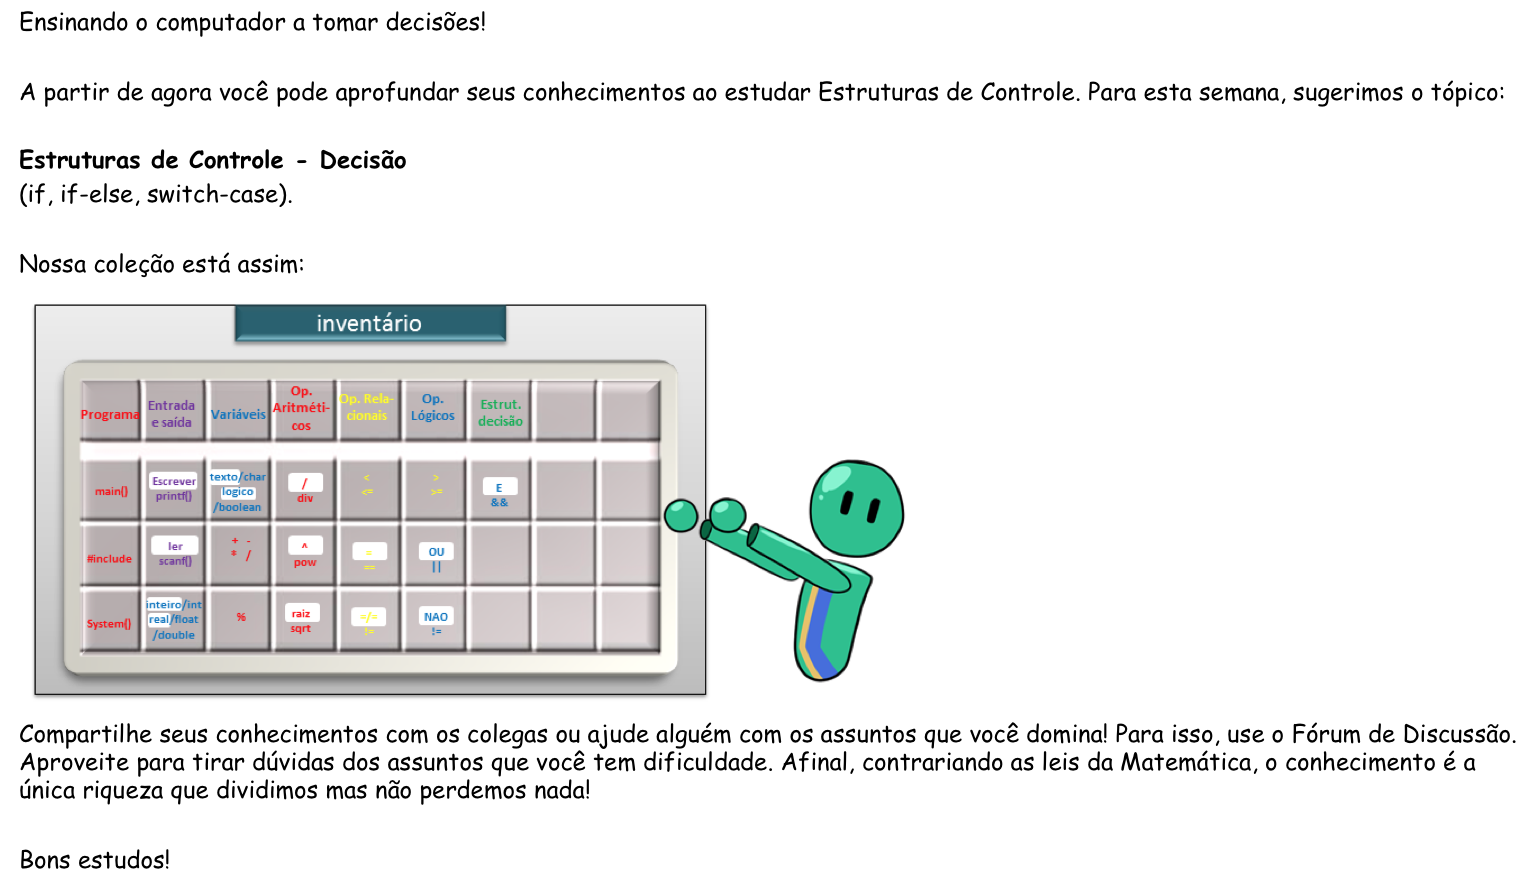
\includegraphics[scale=0.6]{./Figuras/intervencao-6.png}
  \end{center}
  \legend{Fonte: O autor.}
\end{figure}

\begin{figure}[htb]
  \caption{\label{fig:intervencao-7}Intervenção 7 (02/05/18)}
  \begin{center}
      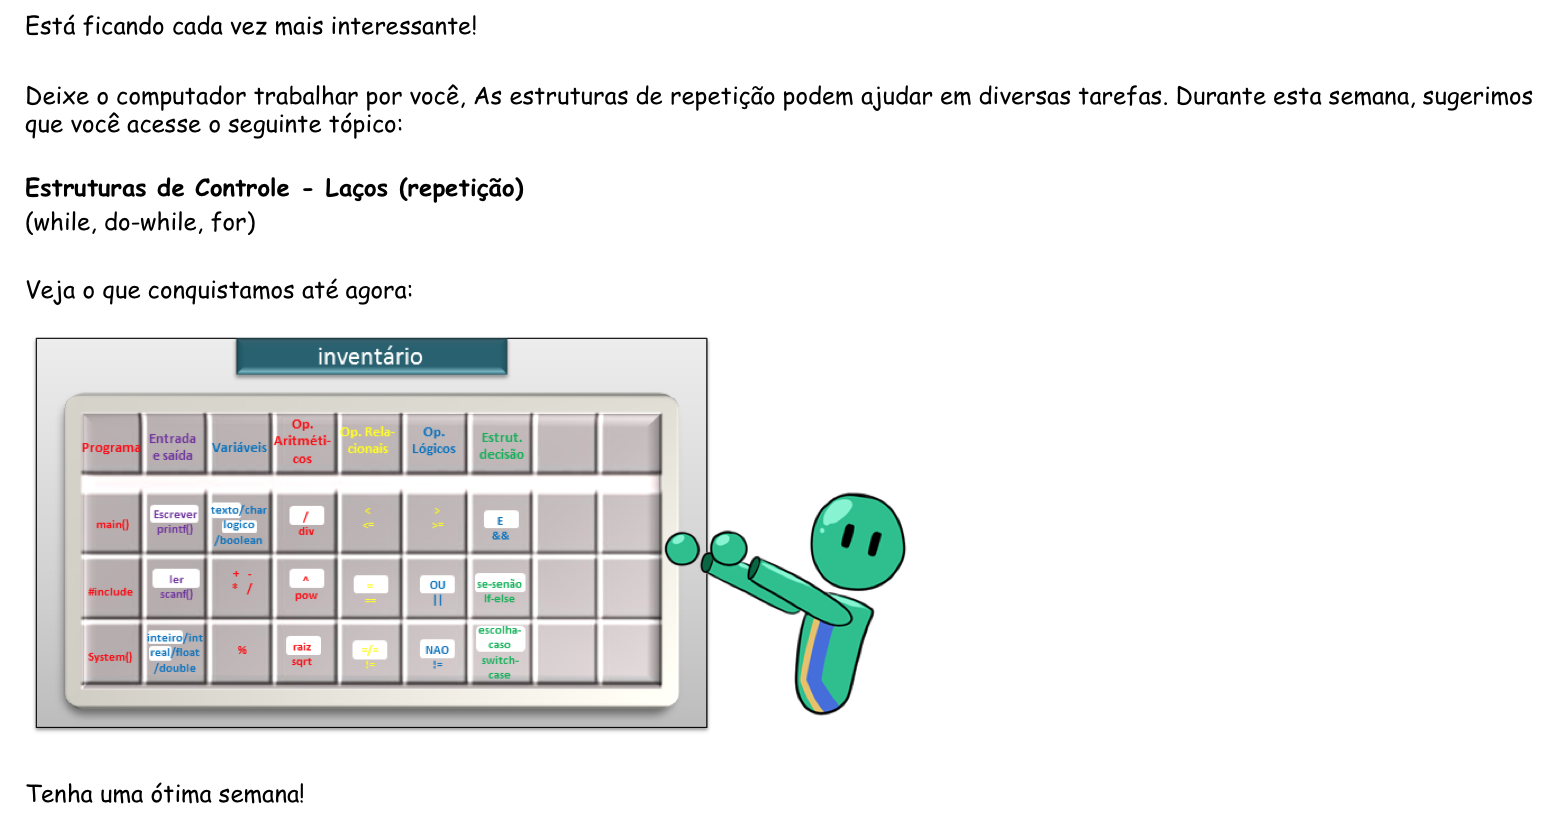
\includegraphics[scale=0.6]{./Figuras/intervencao-7.png}
  \end{center}
  \legend{Fonte: O autor.}
\end{figure}

\begin{figure}[htb]
  \caption{\label{fig:intervencao-8}Intervenção 8 (06/05/18)}
  \begin{center}
      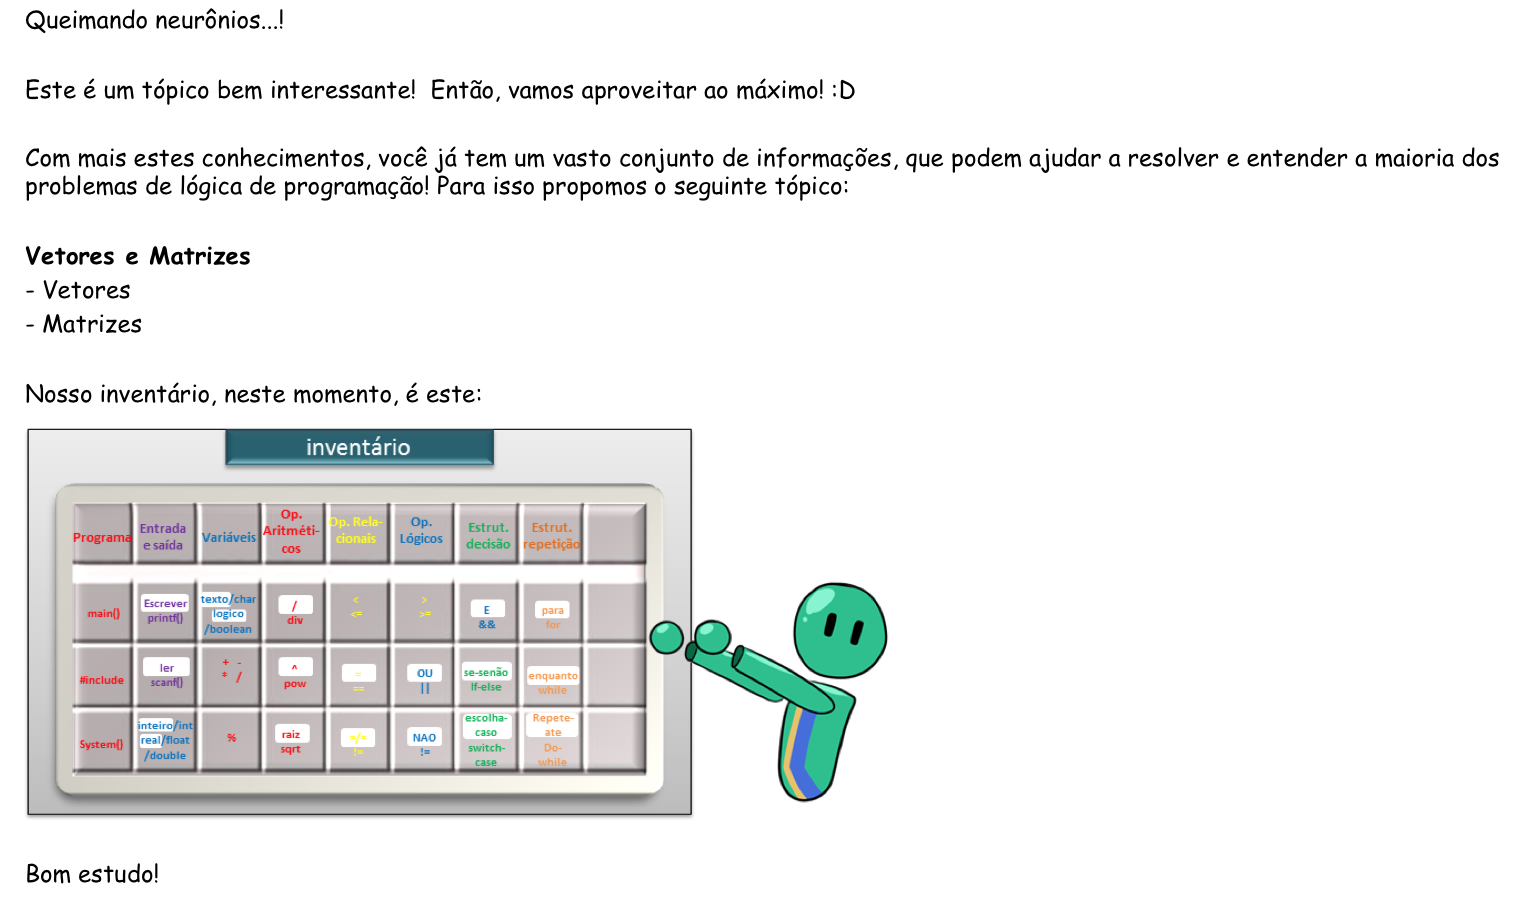
\includegraphics[scale=0.6]{./Figuras/intervencao-8.png}
  \end{center}
  \legend{Fonte: O autor.}
\end{figure}

\begin{figure}[htb]
  \caption{\label{fig:intervencao-9}Intervenção 9 (09/05/18)}
  \begin{center}
      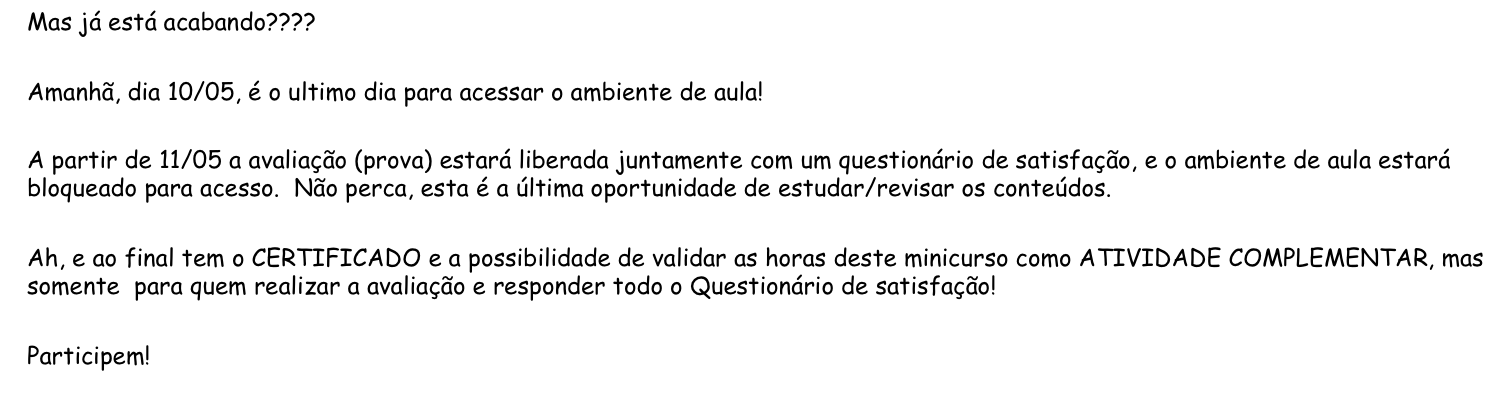
\includegraphics[scale=0.6]{./Figuras/intervencao-9.png}
  \end{center}
  \legend{Fonte: O autor.}
\end{figure}

\begin{figure}[htb]
  \caption{\label{fig:intervencao-10}Intervenção 10 (10/05/18)}
  \begin{center}
      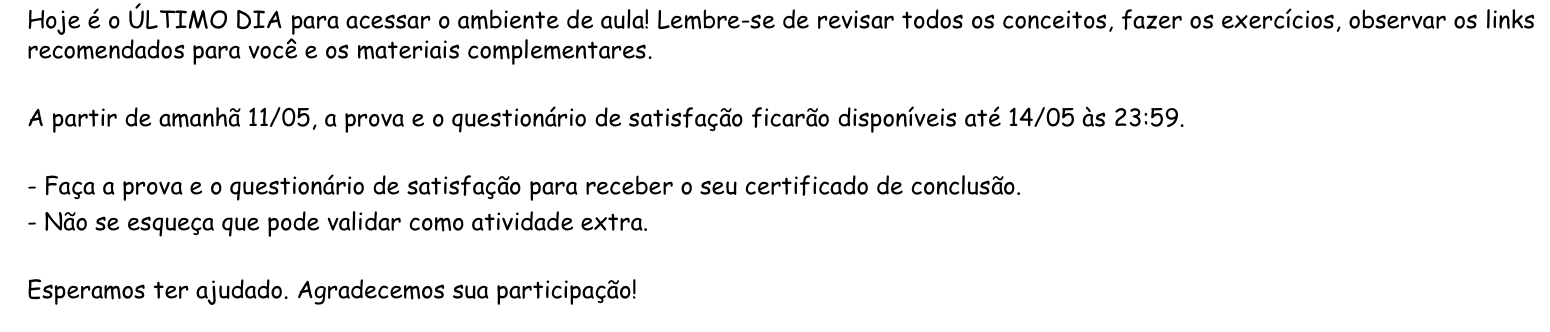
\includegraphics[scale=0.6]{./Figuras/intervencao-10.png}
  \end{center}
  \legend{Fonte: O autor.}
\end{figure}

\begin{figure}[htb]
  \caption{\label{fig:intervencao-11}Intervenção 11 (11/05/18)}
  \begin{center}
      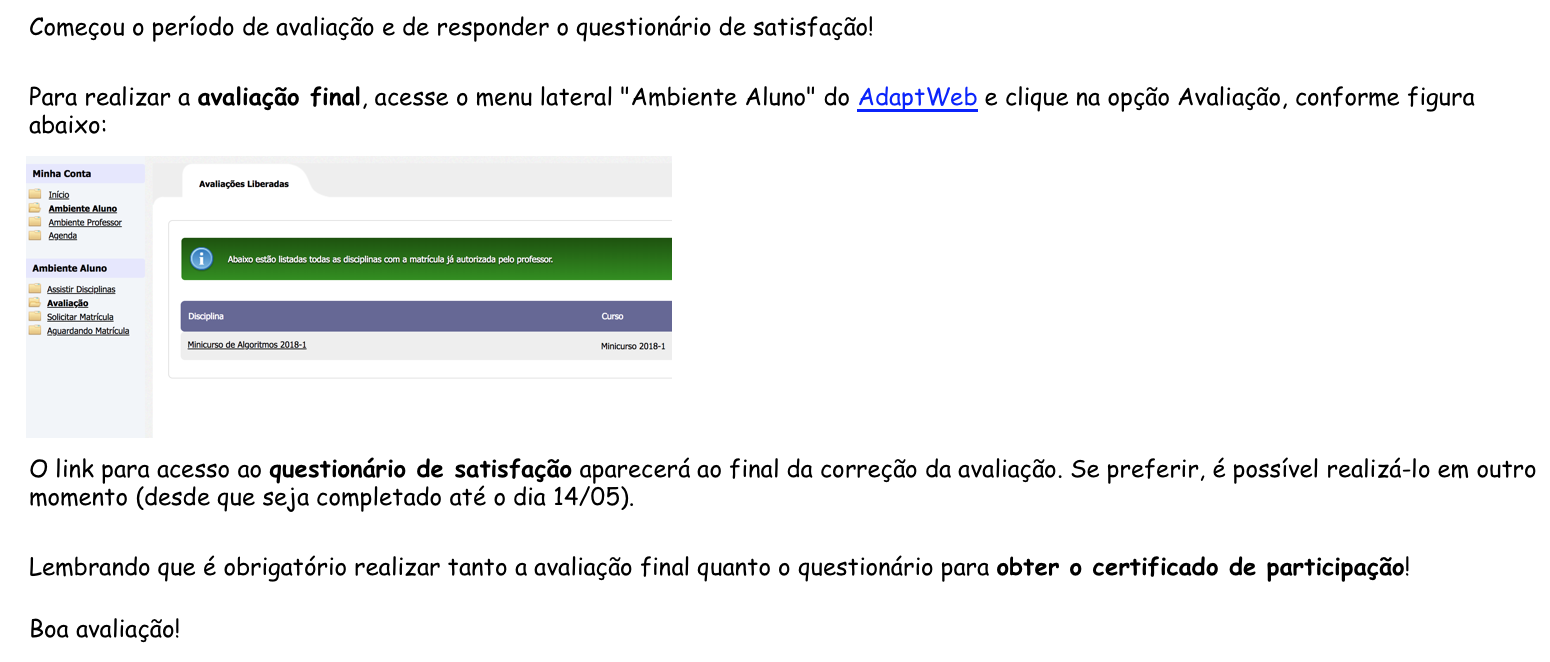
\includegraphics[scale=0.6]{./Figuras/intervencao-11.png}
  \end{center}
  \legend{Fonte: O autor.}
\end{figure}

\begin{figure}[htb]
  \caption{\label{fig:intervencao-12}Intervenção 12 (13/05/18)}
  \begin{center}
      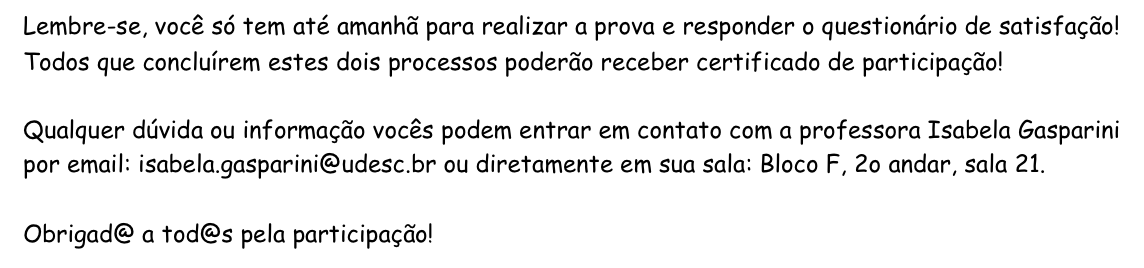
\includegraphics[scale=0.6]{./Figuras/intervencao-12.png}
  \end{center}
  \legend{Fonte: O autor.}
\end{figure}

  \chapter{Análise Estatística das Questões do Questionário}\label{ape:analise-estatistica-questionario}

\textbf{Questão 1: Os itens recomendados corresponderam com os meus interesses.}

\begin{figure}[htb]
  \caption{\label{fig:questao1-boxplot}Boxplot da questão 1}
  \begin{center}
      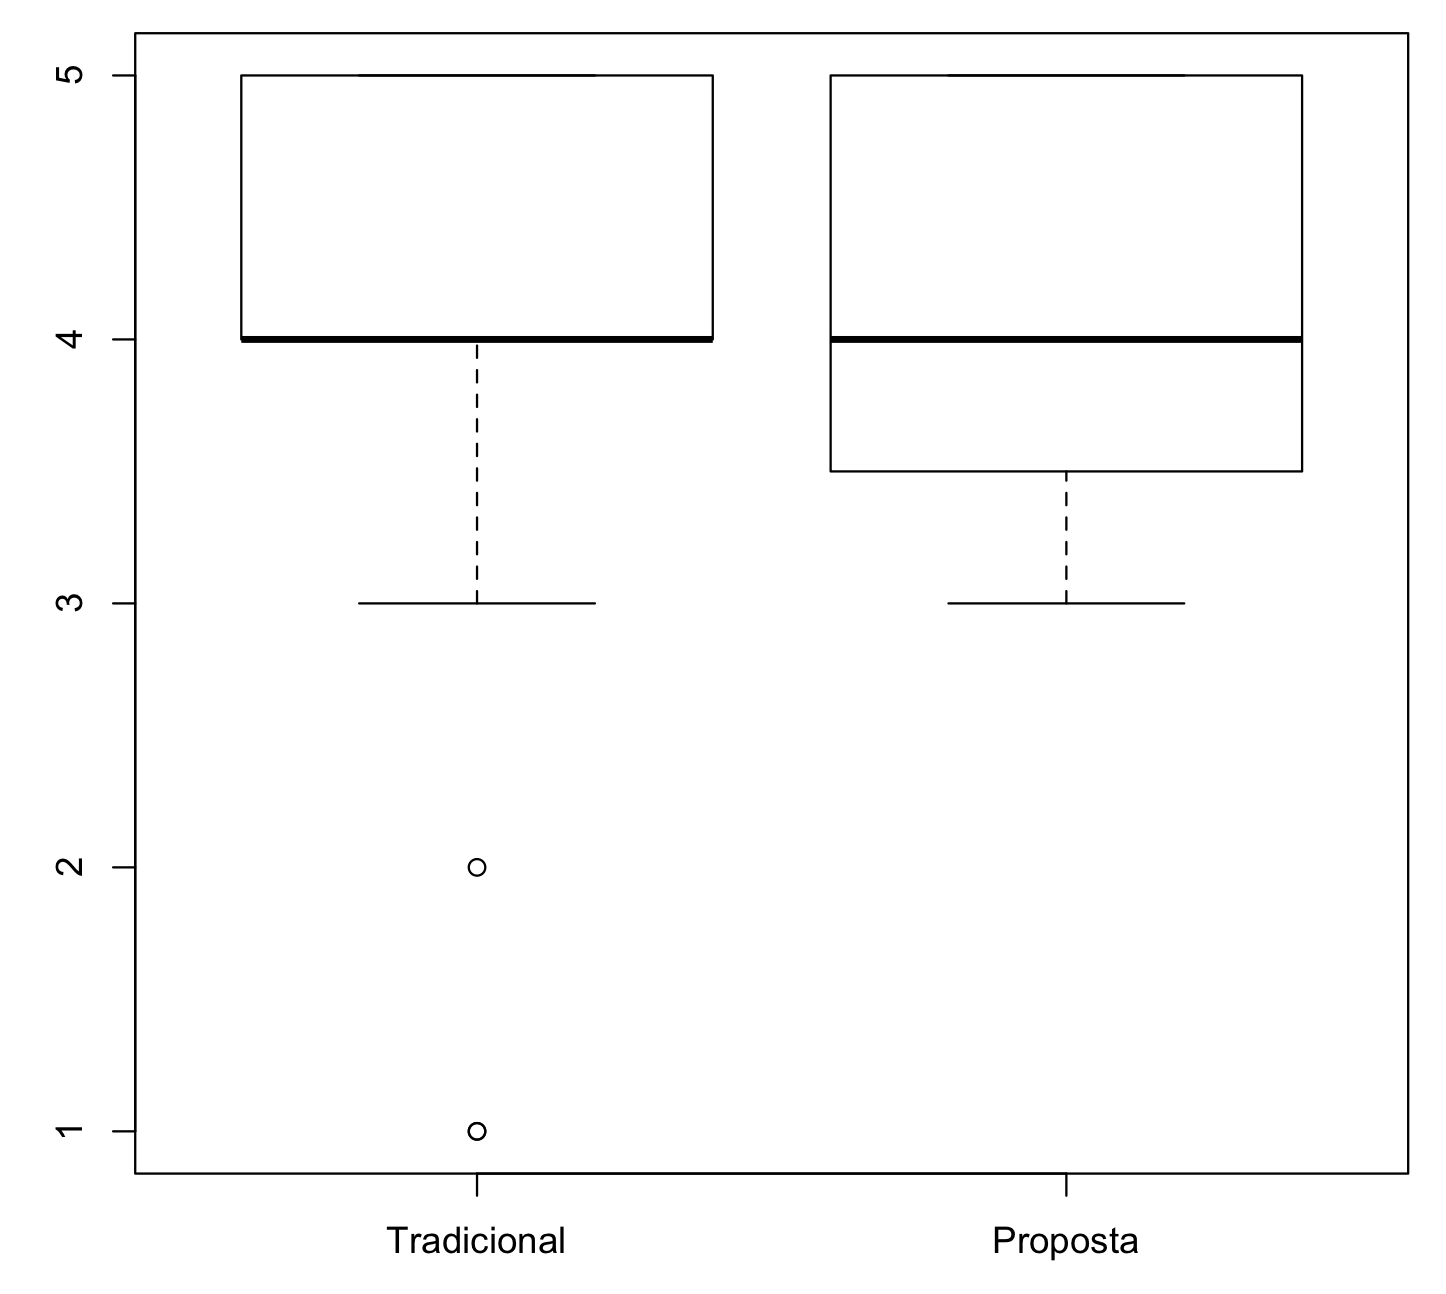
\includegraphics[scale=0.4]{./Figuras/questao1-boxplot.png}
  \end{center}
  \legend{Fonte: O autor.}
\end{figure}

\begin{multicols}{2}

\noindent\textbf{Tradicional}\\
Min.   :1.000\\
1st Qu.:4.000\\
Median :4.000\\
Mean   :4.032\\
3rd Qu.:5.000\\
Max.   :5.000\\
\columnbreak

\noindent\textbf{Proposta}\\
Min.   :3.000\\
1st Qu.:3.750\\
Median :4.000\\
Mean   :4.042\\
3rd Qu.:5.000\\
Max.   :5.000
\end{multicols}

Wilcoxon rank sum test with continuity correction

\noindent
data:  $data\_1\_tradicional$ and $data\_1\_proposta$\\
W = 404, p-value = 0.5635\\
alternative hypothesis: true location shift is not equal to 0

\textbf{Resultado: Aceita a hipótese nula - Sem diferença significativa}

\newpage
\textbf{Questão 2: Os itens recomendados para mim são diversificados (o sistema se preocupa em trazer itens diferentes a cada recomendação).}

\begin{figure}[htb]
  \caption{\label{fig:questao2-boxplot}Boxplot da questão 2}
  \begin{center}
      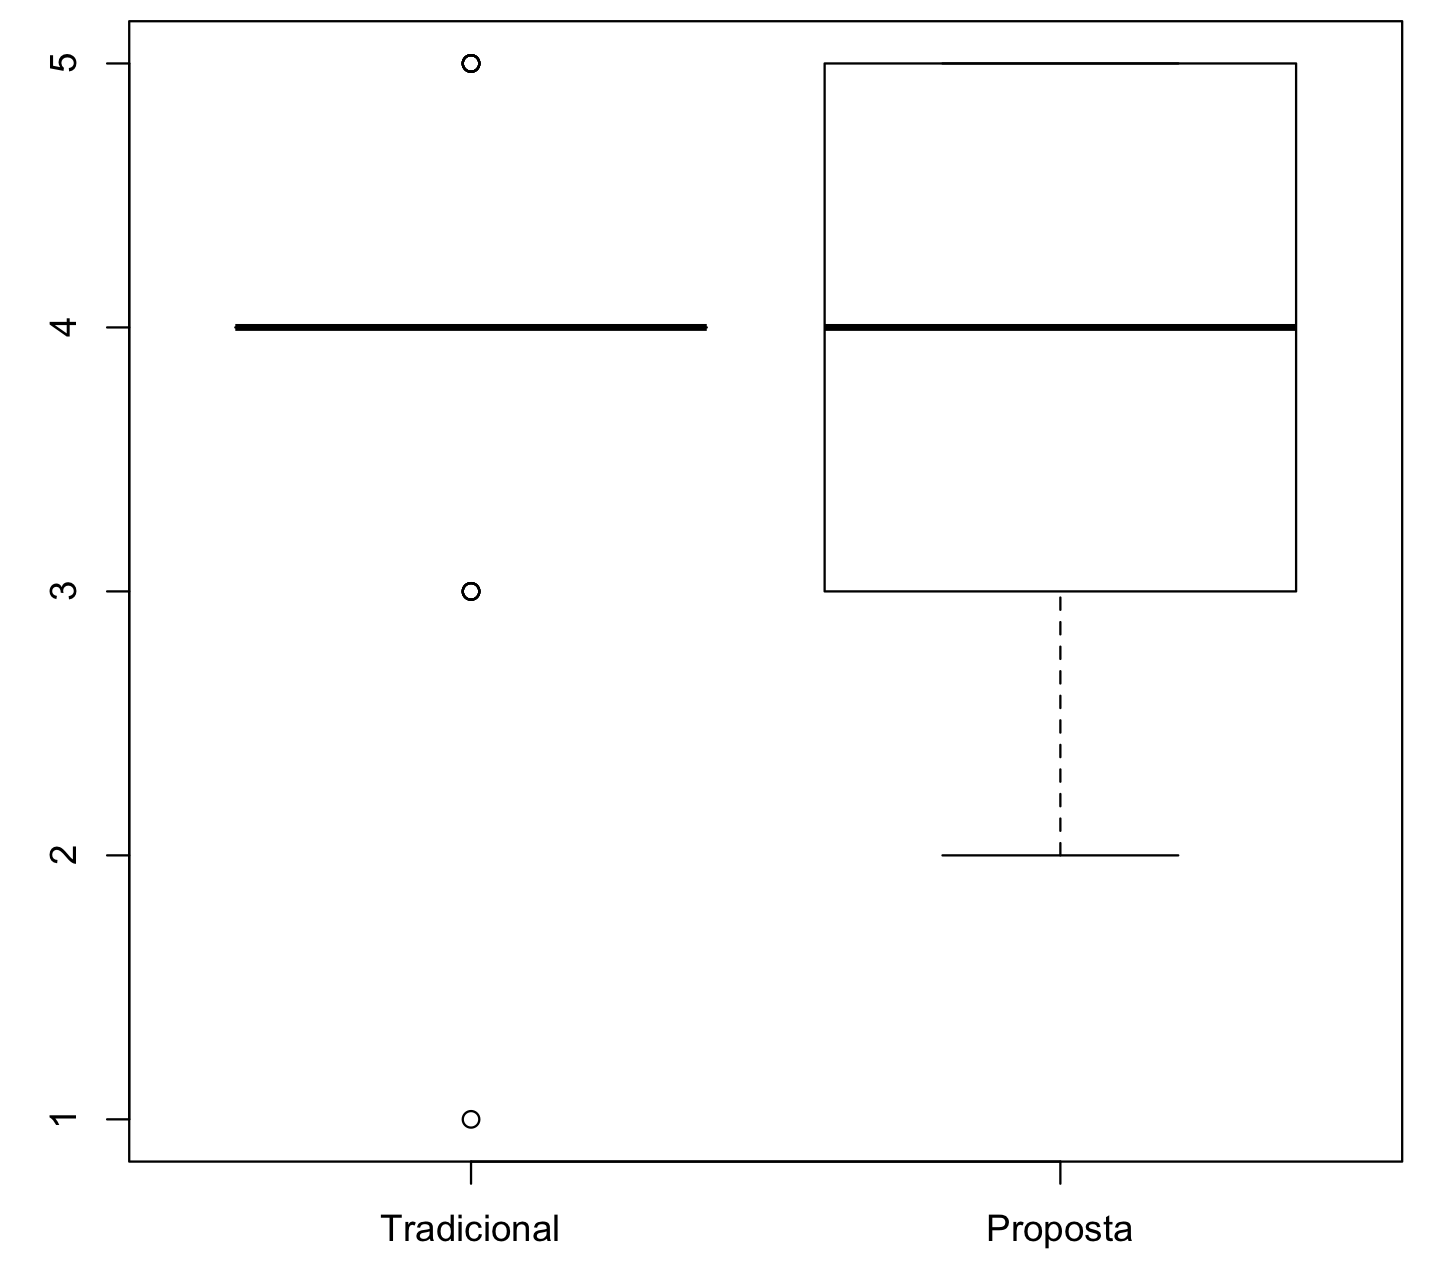
\includegraphics[scale=0.4]{./Figuras/questao2-boxplot.png}
  \end{center}
  \legend{Fonte: O autor.}
\end{figure}

\begin{multicols}{2}

\noindent\textbf{Tradicional}\\
Min.   :1.000\\
1st Qu.:4.000\\
Median :4.000\\
Mean   :3.933\\
3rd Qu.:4.000\\
Max.   :5.000\\
\columnbreak

\noindent\textbf{Proposta}\\
Min.   :2\\
1st Qu.:3\\
Median :4\\
Mean   :4\\
3rd Qu.:5\\
Max.   :5
\end{multicols}

Wilcoxon rank sum test with continuity correction

\noindent
data:  $data\_2\_tradicional$ and $data\_2\_proposta$\\
W = 376.5, p-value = 0.8178\\
alternative hypothesis: true location shift is not equal to 0

\textbf{Resultado: Aceita a hipótese nula - Sem diferença significativa}

\newpage
\textbf{Questão 3: Os itens recomendados corresponderam aos  interesses e necessidades que eu tinha no momento.}

\begin{figure}[htb]
  \caption{\label{fig:questao3-boxplot}Boxplot da questão 3}
  \begin{center}
      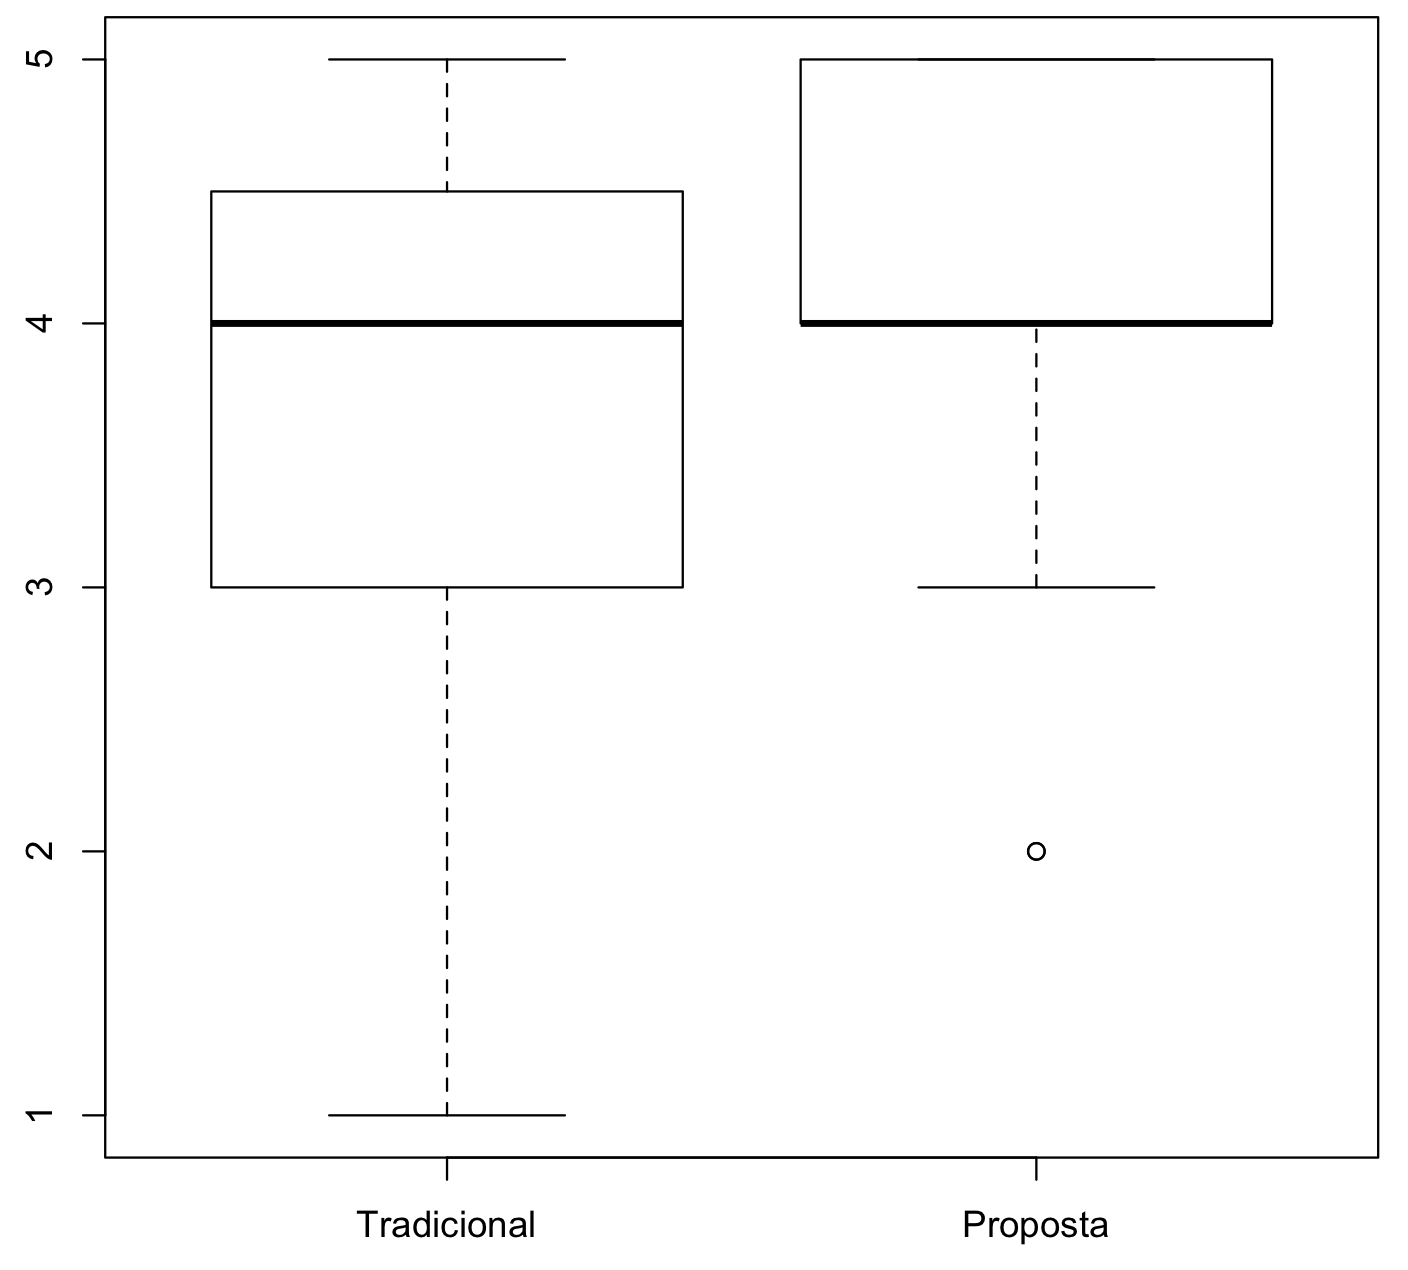
\includegraphics[scale=0.4]{./Figuras/questao3-boxplot.png}
  \end{center}
  \legend{Fonte: O autor.}
\end{figure}

\begin{multicols}{2}

\noindent\textbf{Tradicional}\\
Min.   :1.000\\
1st Qu.:3.000\\
Median :4.000\\
Mean   :3.806\\
3rd Qu.:4.500\\
Max.   :5.000\\
\columnbreak

\noindent\textbf{Proposta}\\
Min.   :2\\
1st Qu.:4\\
Median :4\\
Mean   :4\\
3rd Qu.:5\\
Max.   :5
\end{multicols}

Wilcoxon rank sum test with continuity correction

\noindent
data:  $data\_3\_tradicional$ and $data\_3\_proposta$\\
W = 364, p-value = 0.5119\\
alternative hypothesis: true location shift is not equal to 0

\textbf{Resultado: Aceita a hipótese nula - Sem diferença significativa}

\newpage
\textbf{Questão 4: As recomendações são feitas no momento adequado.}

\begin{figure}[htb]
  \caption{\label{fig:questao4-boxplot}Boxplot da questão 4}
  \begin{center}
      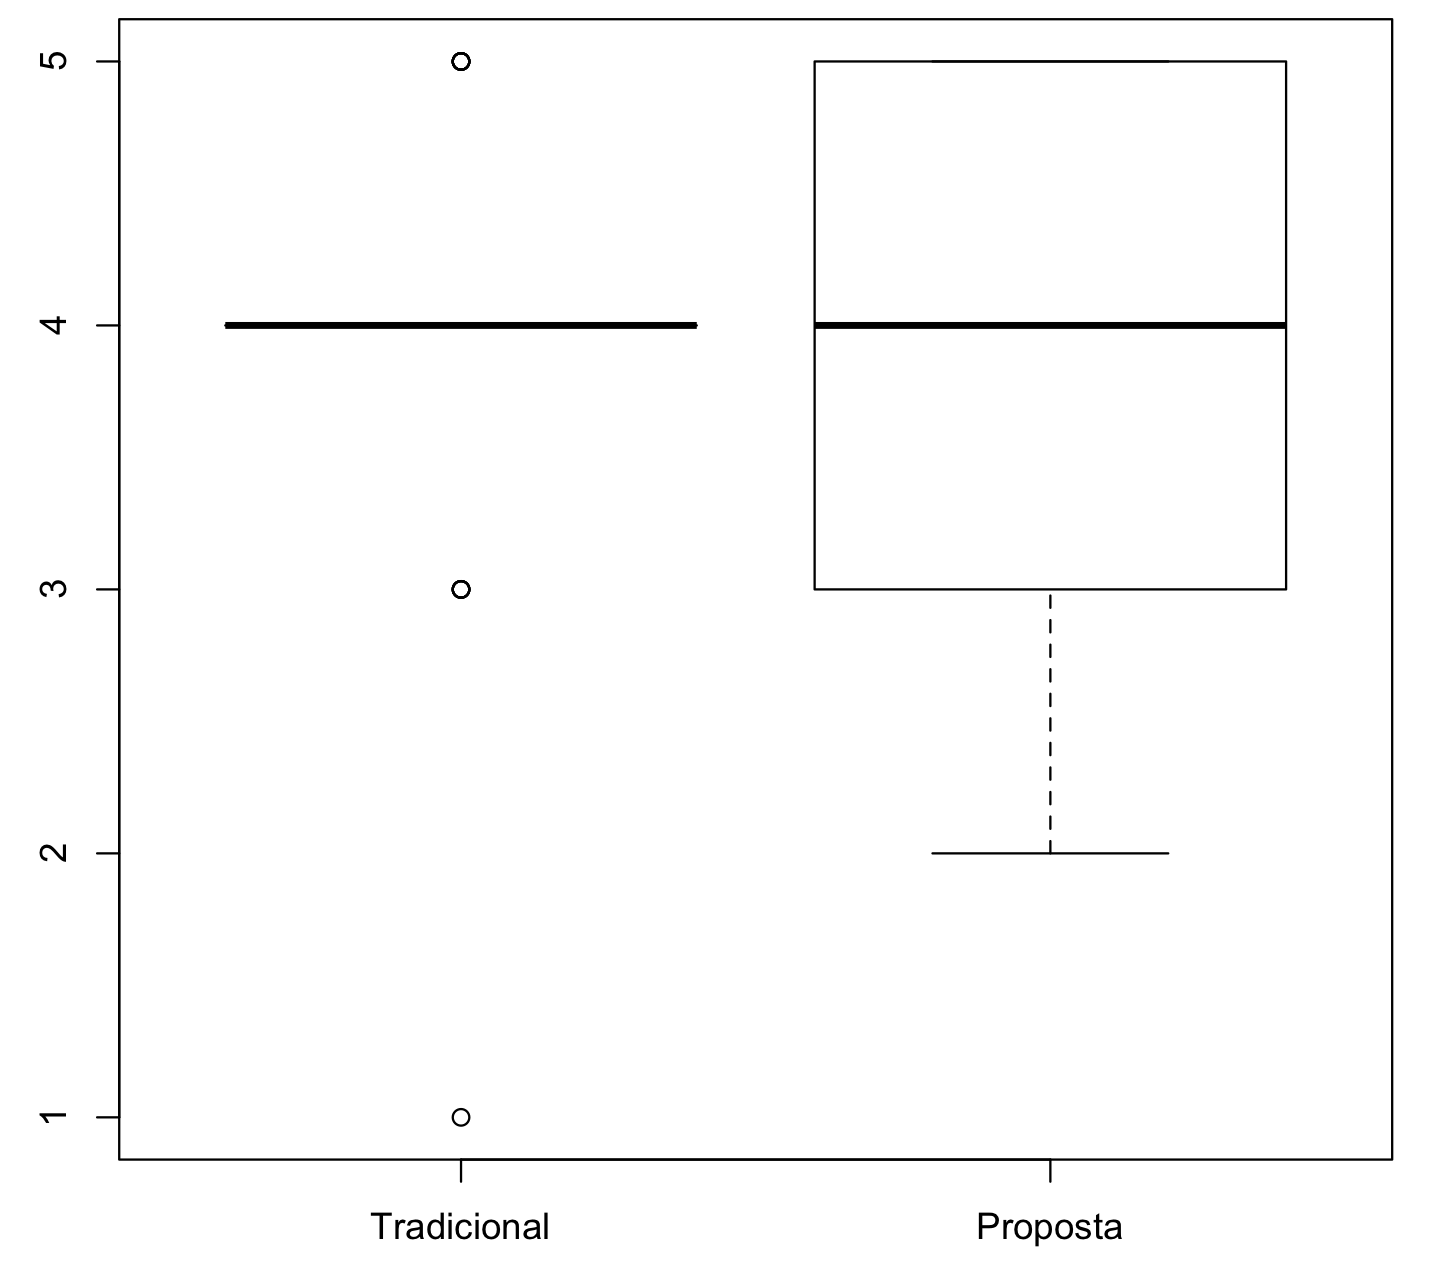
\includegraphics[scale=0.4]{./Figuras/questao4-boxplot.png}
  \end{center}
  \legend{Fonte: O autor.}
\end{figure}

\begin{multicols}{2}

\noindent\textbf{Tradicional}\\
Min.   :1.000\\
1st Qu.:4.000\\
Median :4.000\\
Mean   :3.931\\
3rd Qu.:4.000\\
Max.   :5.000\\
\columnbreak

\noindent\textbf{Proposta}\\
Min.   :2\\
1st Qu.:3\\
Median :4\\
Mean   :4\\
3rd Qu.:5\\
Max.   :5
\end{multicols}

Wilcoxon rank sum test with continuity correction

\noindent
data:  $data\_4\_tradicional$ and $data\_4\_proposta$\\
W = 378, p-value = 0.8198\\
alternative hypothesis: true location shift is not equal to 0

\textbf{Resultado: Aceita a hipótese nula - Sem diferença significativa}

\newpage
\textbf{Questão 5: O sistema de recomendação explica porque os links são recomendados para mim.}

\begin{figure}[htb]
  \caption{\label{fig:questao5-boxplot}Boxplot da questão 5}
  \begin{center}
      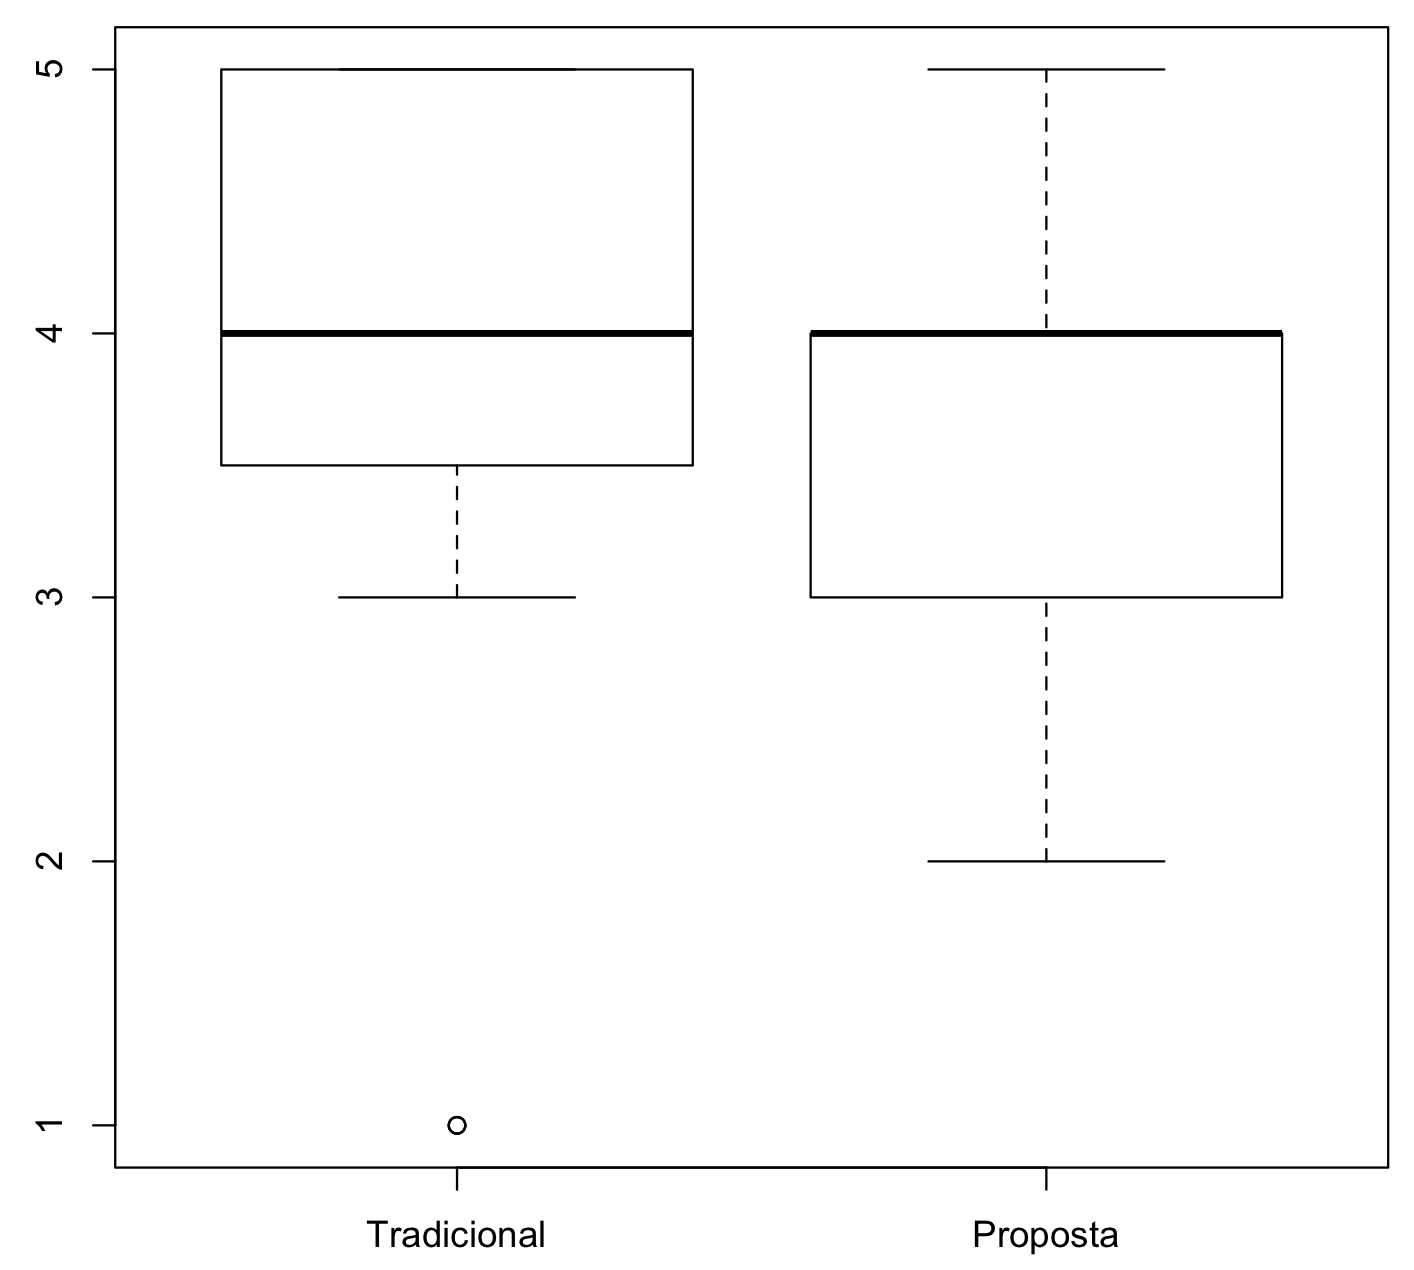
\includegraphics[scale=0.4]{./Figuras/questao5-boxplot.png}
  \end{center}
  \legend{Fonte: O autor.}
\end{figure}

\begin{multicols}{2}

\noindent\textbf{Tradicional}\\
Min.   :1.000\\
1st Qu.:3.500\\
Median :4.000\\
Mean   :3.889\\
3rd Qu.:5.000\\
Max.   :5.000\\
\columnbreak

\noindent\textbf{Proposta}\\
Min.   :2.00\\
1st Qu.:3.00\\
Median :4.00\\
Mean   :3.72\\
3rd Qu.:4.00\\
Max.   :5.00
\end{multicols}

Wilcoxon rank sum test with continuity correction

\noindent
data:  $data\_5\_tradicional$ and $data\_5\_proposta$\\
W = 396, p-value = 0.2665\\
alternative hypothesis: true location shift is not equal to 0

\textbf{Resultado: Aceita a hipótese nula - Sem diferença significativa}

\newpage
\textbf{Questão 6: A informação apresentada na interface para os itens recomendados é suficiente para mim.}

\begin{figure}[htb]
  \caption{\label{fig:questao6-boxplot}Boxplot da questão 6}
  \begin{center}
      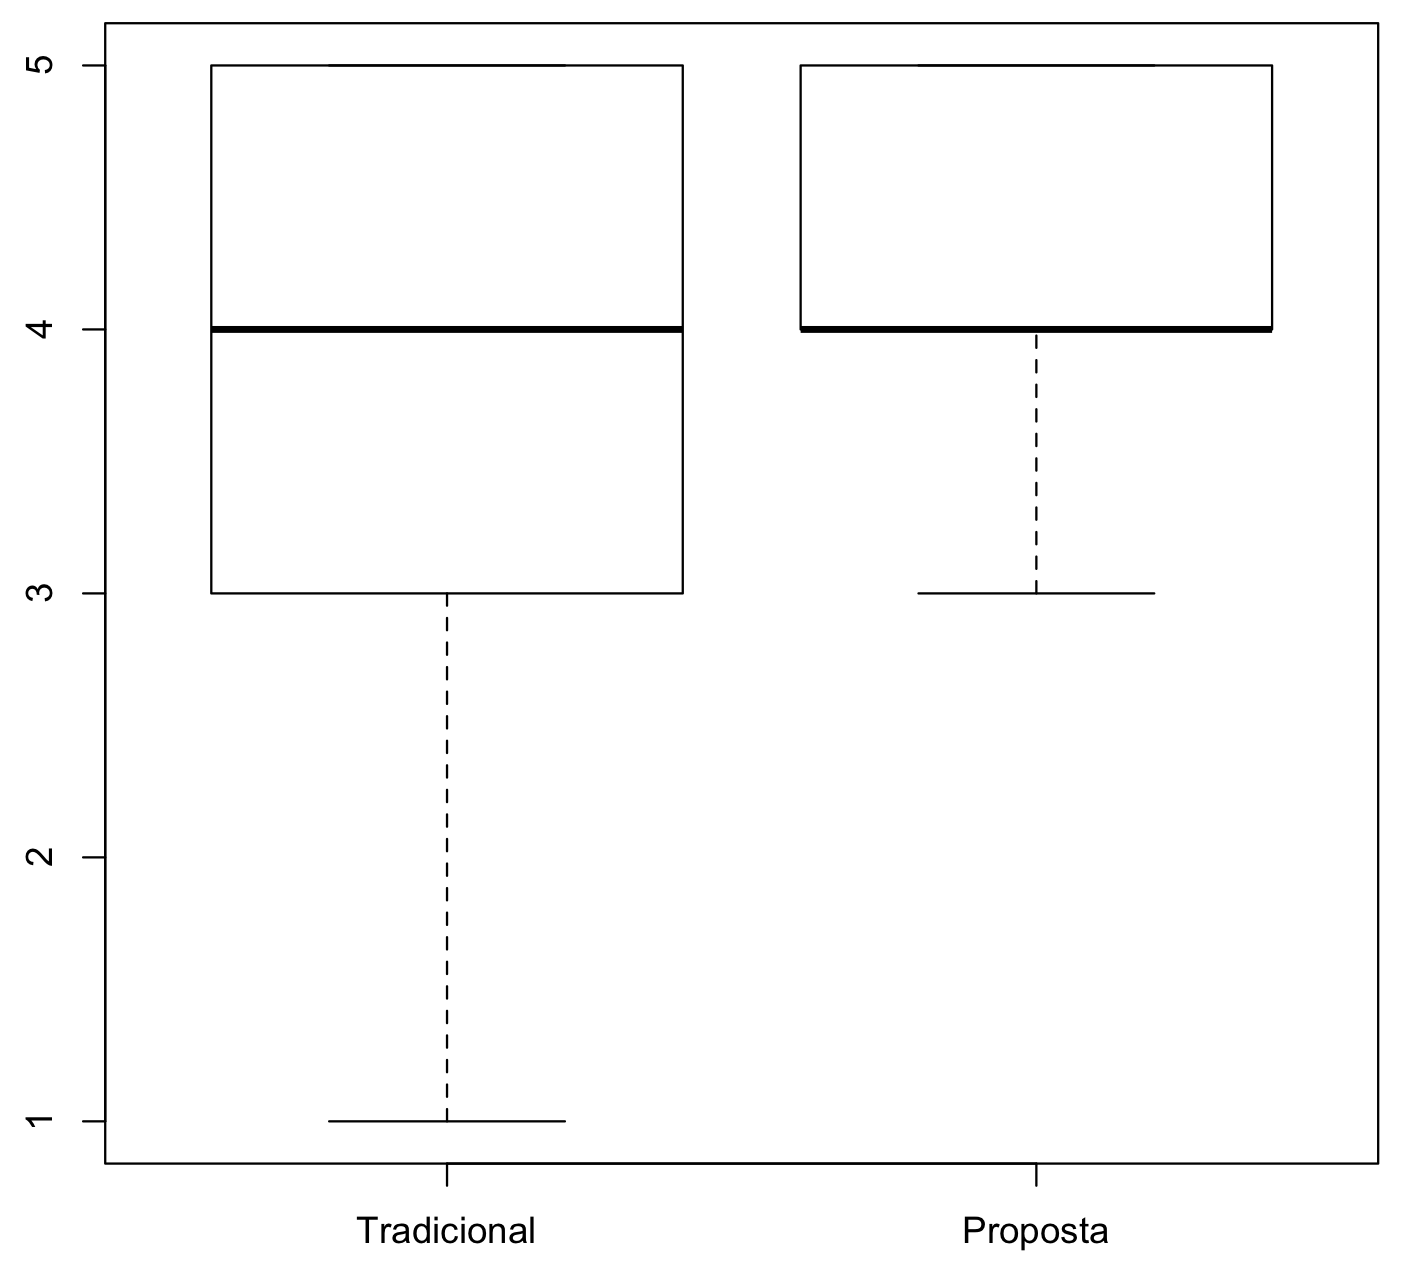
\includegraphics[scale=0.4]{./Figuras/questao6-boxplot.png}
  \end{center}
  \legend{Fonte: O autor.}
\end{figure}

\begin{multicols}{2}

\noindent\textbf{Tradicional}\\
Min.   :1.000\\
1st Qu.:3.000\\
Median :4.000\\
Mean   :3.655\\
3rd Qu.:5.000\\
Max.   :5.000\\
\columnbreak

\noindent\textbf{Proposta}\\
Min.   :3.000\\
1st Qu.:4.000\\
Median :4.000\\
Mean   :4.192\\
3rd Qu.:5.000\\
Max.   :5.000
\end{multicols}

Wilcoxon rank sum test with continuity correction

\noindent
data:  $data\_6\_tradicional$ and $data\_6\_proposta$\\
W = 301.5, p-value = 0.1799\\
alternative hypothesis: true location shift is not equal to 0

\textbf{Resultado: Aceita a hipótese nula - Sem diferença significativa}

\newpage
\textbf{Questão 7: O layout do sistema de recomendação é atrativo e adequado.}

\begin{figure}[htb]
  \caption{\label{fig:questao7-boxplot}Boxplot da questão 7}
  \begin{center}
      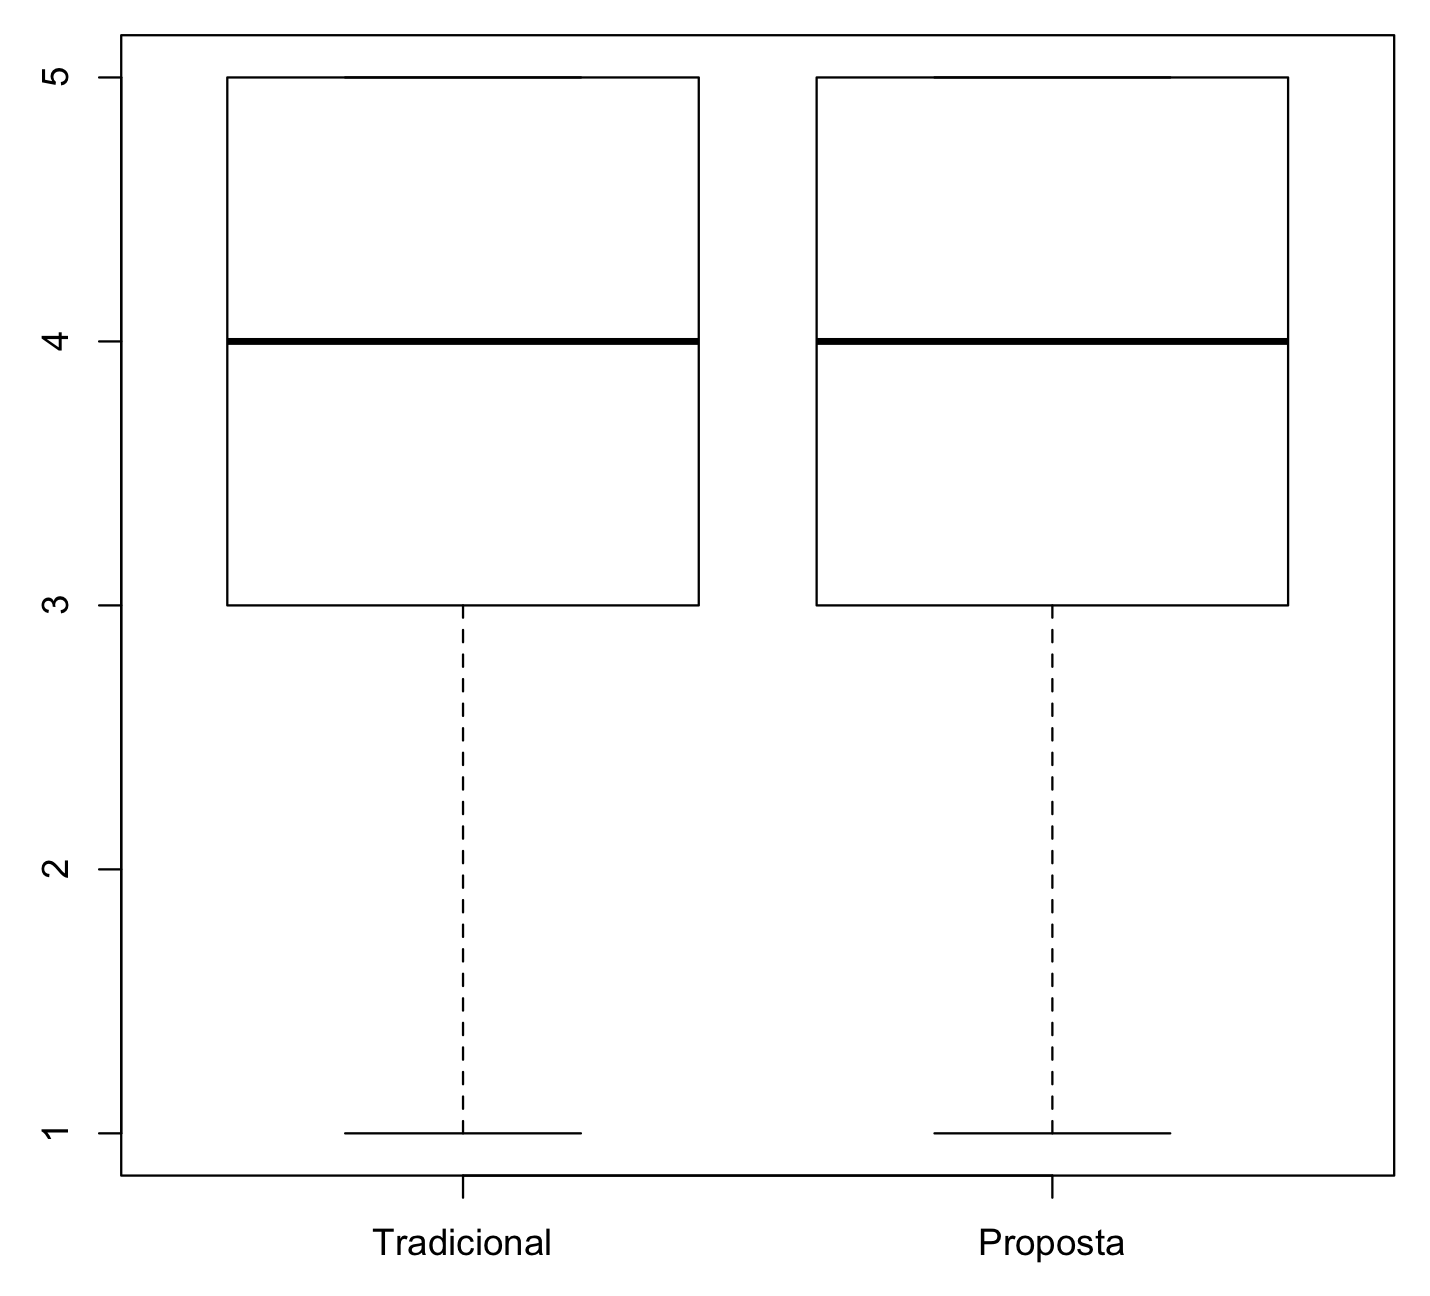
\includegraphics[scale=0.4]{./Figuras/questao7-boxplot.png}
  \end{center}
  \legend{Fonte: O autor.}
\end{figure}

\begin{multicols}{2}

\noindent\textbf{Tradicional}\\
Min.   :1.000\\
1st Qu.:3.000\\
Median :4.000\\
Mean   :3.676\\
3rd Qu.:4.750\\
Max.   :5.000\\
\columnbreak

\noindent\textbf{Proposta}\\
Min.   :1.0\\
1st Qu.:3.0\\
Median :4.0\\
Mean   :3.8\\
3rd Qu.:5.0\\
Max.   :5.0
\end{multicols}

Wilcoxon rank sum test with continuity correction

\noindent
data:  $data\_7\_tradicional$ and $data\_7\_proposta$\\
W = 413, p-value = 0.8536\\
alternative hypothesis: true location shift is not equal to 0

\textbf{Resultado: Aceita a hipótese nula - Sem diferença significativa}

\newpage
\textbf{Questão 8: Eu encontrei facilmente o local onde os itens são recomendados.}

\begin{figure}[htb]
  \caption{\label{fig:questao8-boxplot}Boxplot da questão 8}
  \begin{center}
      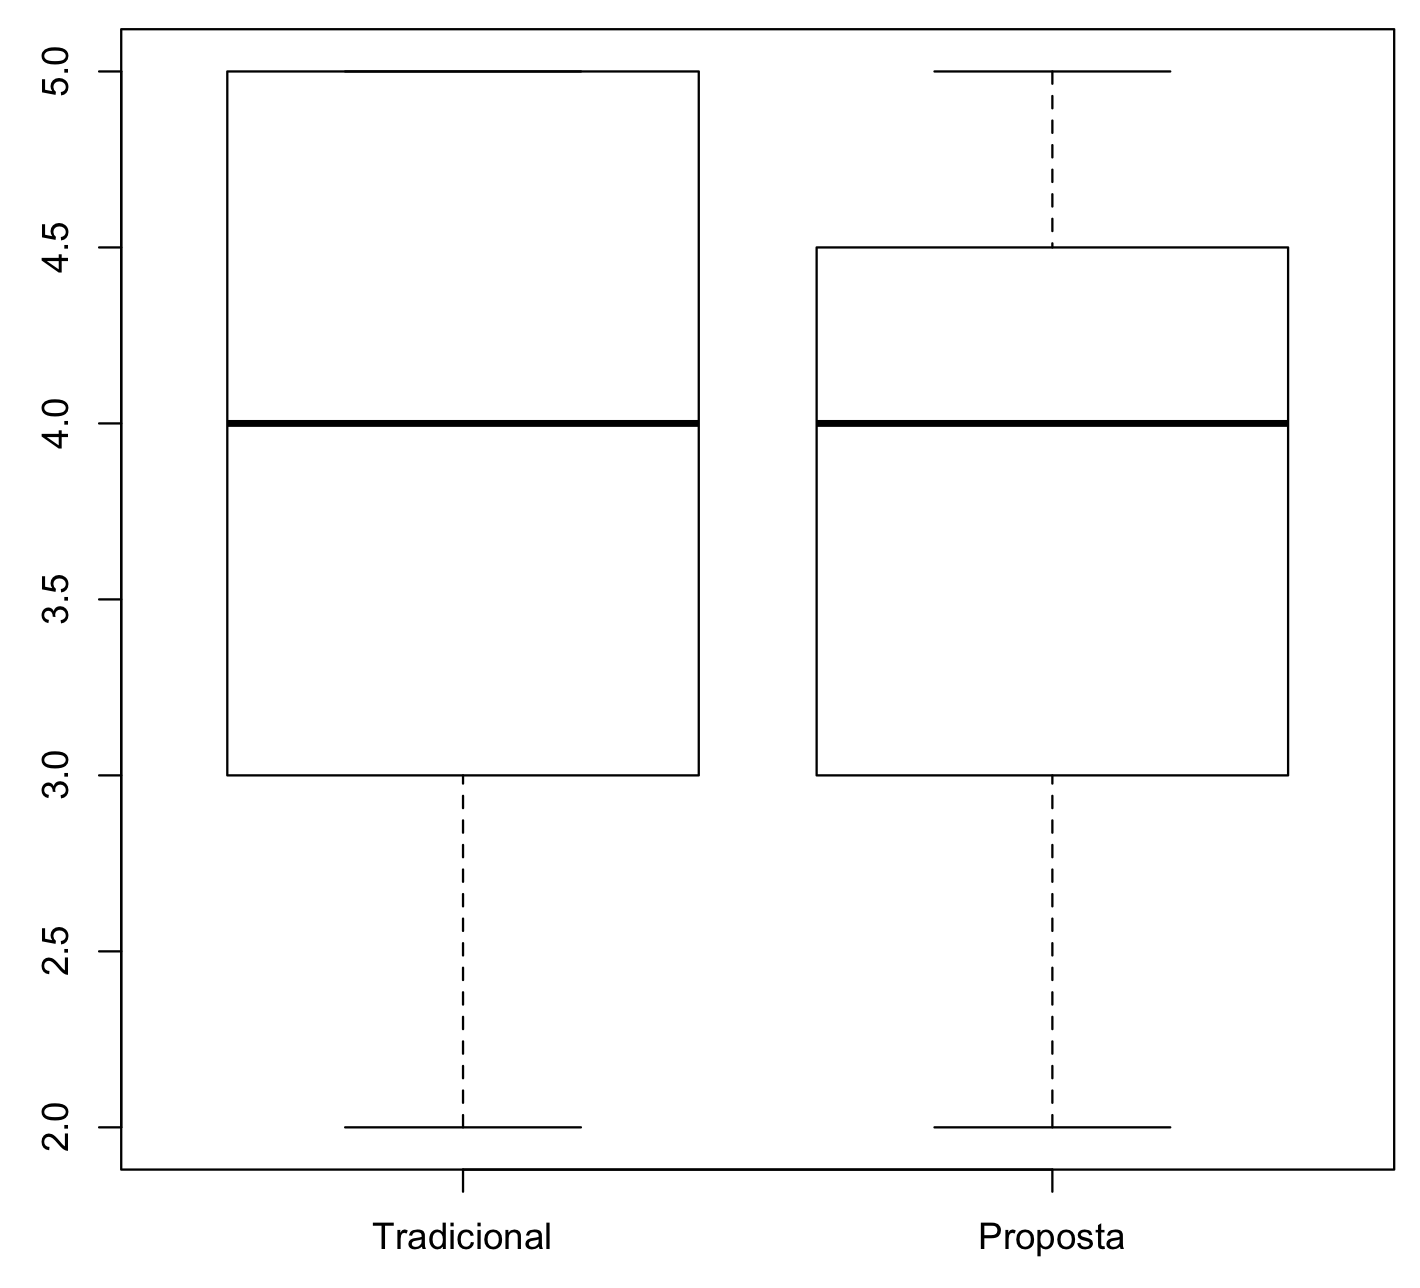
\includegraphics[scale=0.4]{./Figuras/questao8-boxplot.png}
  \end{center}
  \legend{Fonte: O autor.}
\end{figure}

\begin{multicols}{2}

\noindent\textbf{Tradicional}\\
Min.   :2.0\\
1st Qu.:3.0\\
Median :4.0\\
Mean   :3.8\\
3rd Qu.:5.0\\
Max.   :5.0\\
\columnbreak

\noindent\textbf{Proposta}\\
Min.   :2.00\\
1st Qu.:3.00\\
Median :4.00\\
Mean   :3.75\\
3rd Qu.:4.25\\
Max.   :5.00
\end{multicols}

Wilcoxon rank sum test with continuity correction

\noindent
data:  $data\_8\_tradicional$ and $data\_8\_proposta$\\
W = 381, p-value = 0.7093\\
alternative hypothesis: true location shift is not equal to 0

\textbf{Resultado: Aceita a hipótese nula - Sem diferença significativa}

\newpage
\textbf{Questão 9: Eu percebi que o sistema de recomendação aprendia sobre minhas necessidades/preferências conforme eu avançava na disciplina.}

\begin{figure}[htb]
  \caption{\label{fig:questao9-boxplot}Boxplot da questão 9}
  \begin{center}
      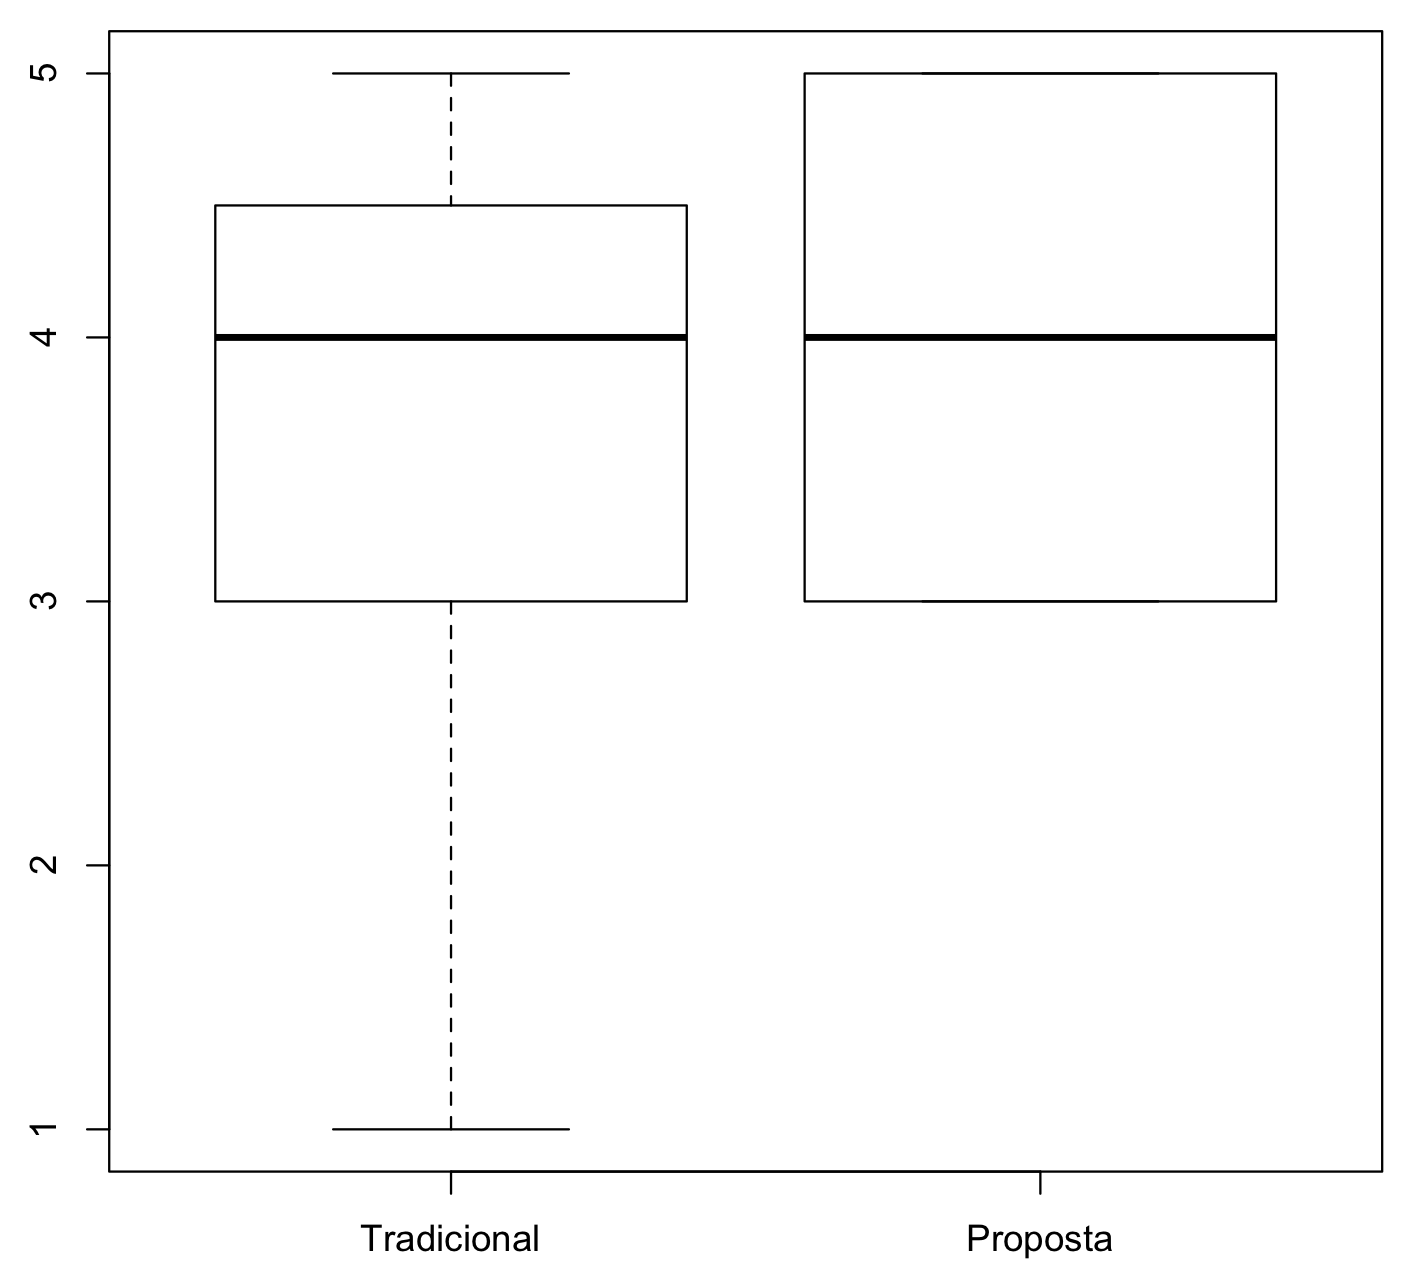
\includegraphics[scale=0.4]{./Figuras/questao9-boxplot.png}
  \end{center}
  \legend{Fonte: O autor.}
\end{figure}

\begin{multicols}{2}

\noindent\textbf{Tradicional}\\
Min.   :1.000\\
1st Qu.:3.000\\
Median :4.000\\
Mean   :3.643\\
3rd Qu.:4.250\\
Max.   :5.000\\
\columnbreak

\noindent\textbf{Proposta}\\
Min.   :3.000\\
1st Qu.:3.000\\
Median :4.000\\
Mean   :3.875\\
3rd Qu.:5.000\\
Max.   :5.000
\end{multicols}

Wilcoxon rank sum test with continuity correction

\noindent
data:  $data\_9\_tradicional$ and $data\_9\_proposta$\\
W = 313.5, p-value = 0.6722\\
alternative hypothesis: true location shift is not equal to 0

\textbf{Resultado: Aceita a hipótese nula - Sem diferença significativa}

\newpage
\textbf{Questão 10: É facil encontrar um item para estudar com a ajuda do sistema de recomendação.}

\begin{figure}[htb]
  \caption{\label{fig:questao10-boxplot}Boxplot da questão 10}
  \begin{center}
      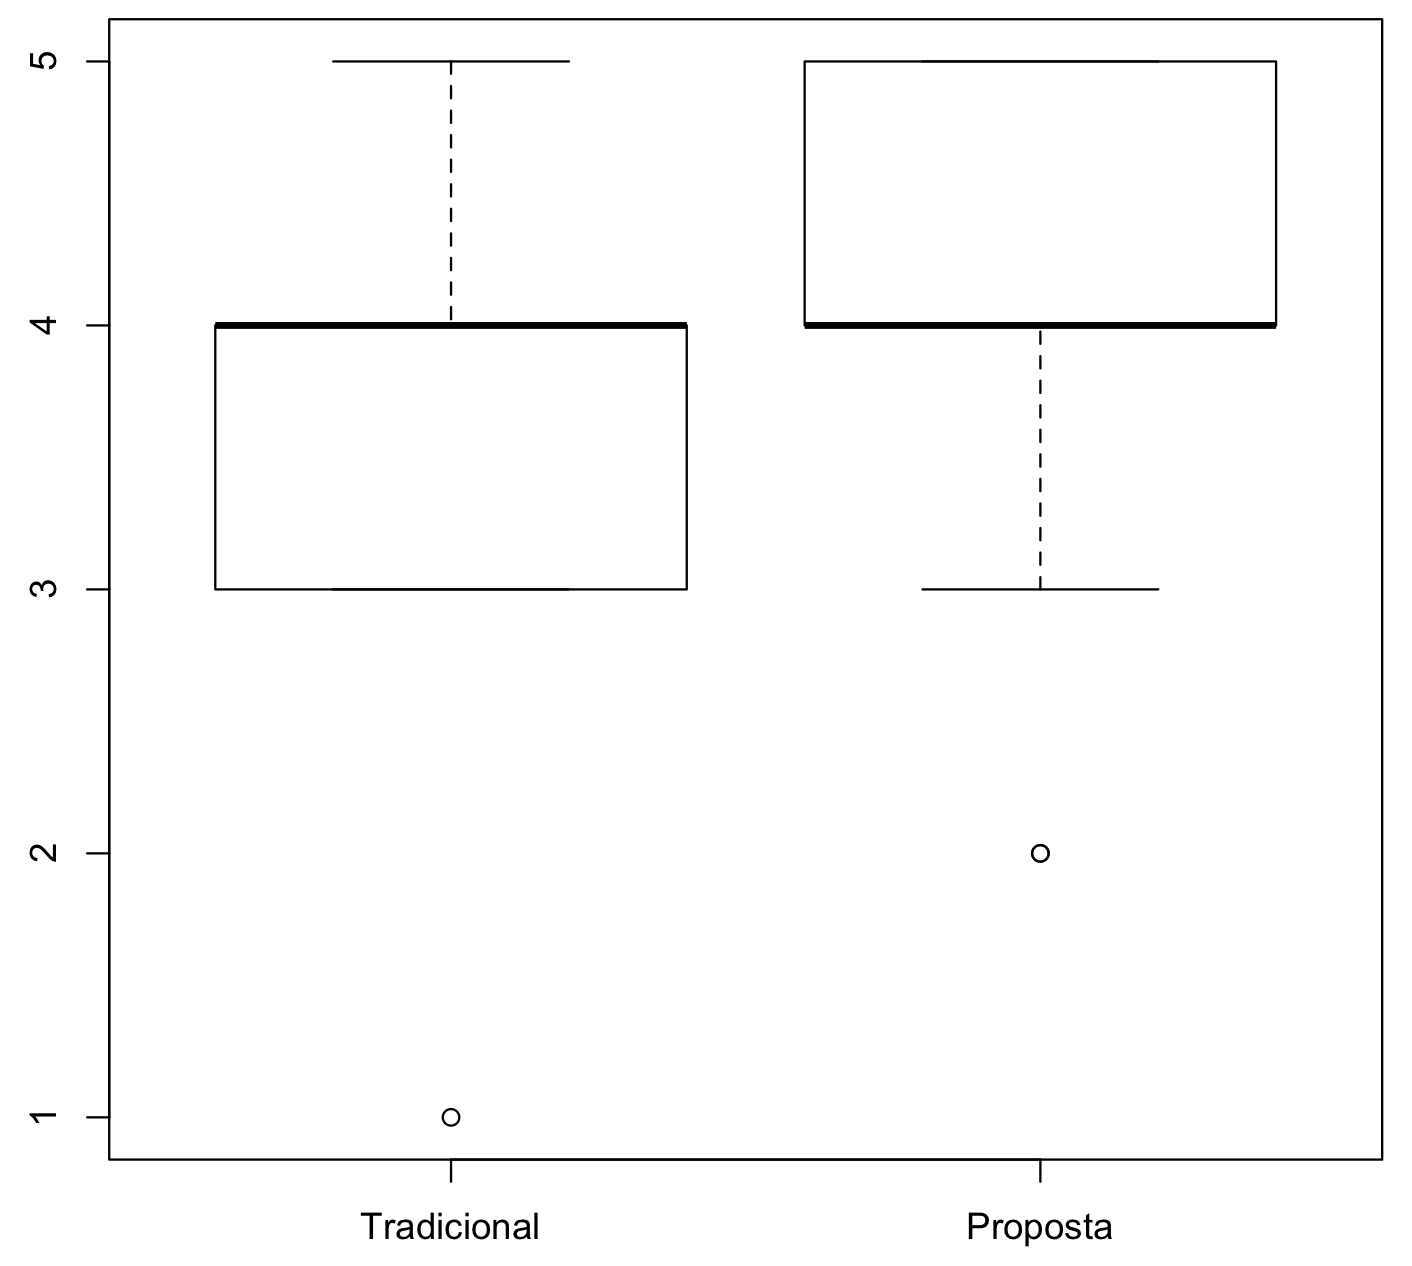
\includegraphics[scale=0.4]{./Figuras/questao10-boxplot.png}
  \end{center}
  \legend{Fonte: O autor.}
\end{figure}

\begin{multicols}{2}

\noindent\textbf{Tradicional}\\
Min.   :1.00\\
1st Qu.:3.00\\
Median :4.00\\
Mean   :3.69\\
3rd Qu.:4.00\\
Max.   :5.00\\
\columnbreak

\noindent\textbf{Proposta}\\
Min.   :2\\
1st Qu.:4\\
Median :4\\
Mean   :4\\
3rd Qu.:5\\
Max.   :5
\end{multicols}

Wilcoxon rank sum test with continuity correction

\noindent
data:  $data\_10\_tradicional$ and $data\_10\_proposta$\\
W = 296, p-value = 0.1452\\
alternative hypothesis: true location shift is not equal to 0

\textbf{Resultado: Aceita a hipótese nula - Sem diferença significativa}

\newpage
\textbf{Questão 11: Eu me senti apoiado para encontrar itens do meu interesse com a ajuda do sistema de recomendação.}

\begin{figure}[htb]
  \caption{\label{fig:questao11-boxplot}Boxplot da questão 11}
  \begin{center}
      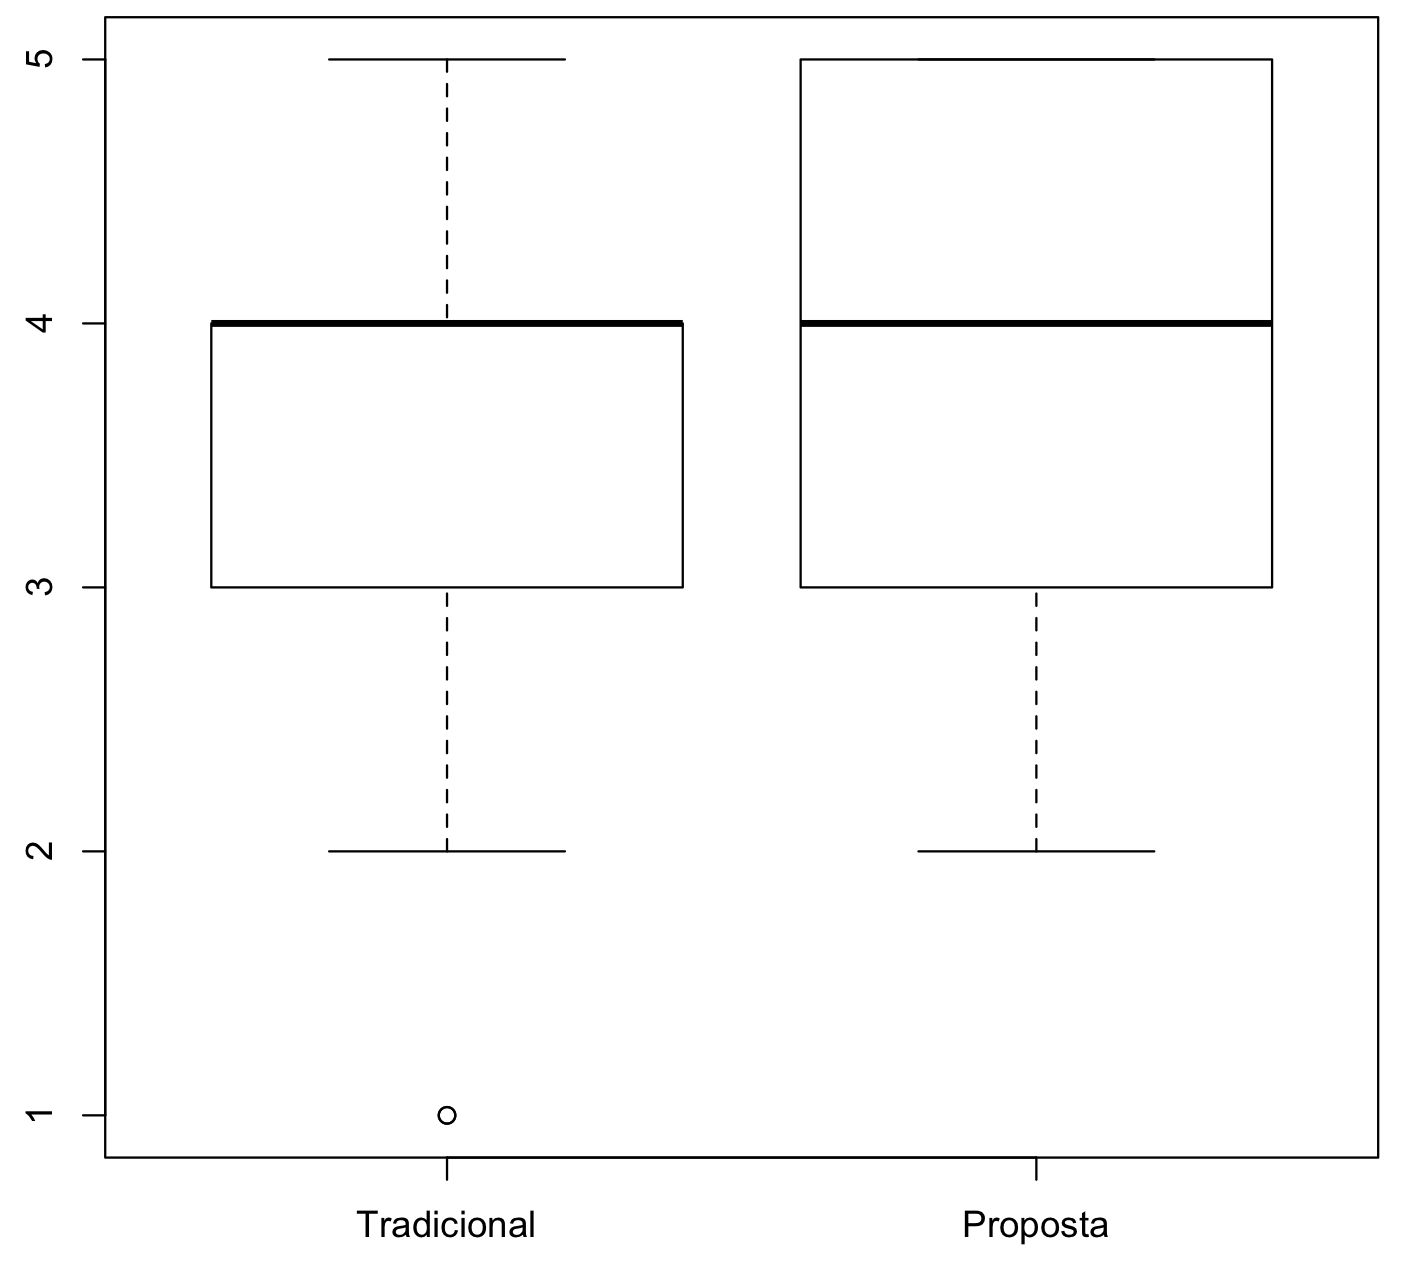
\includegraphics[scale=0.4]{./Figuras/questao11-boxplot.png}
  \end{center}
  \legend{Fonte: O autor.}
\end{figure}

\begin{multicols}{2}

\noindent\textbf{Tradicional}\\
Min.   :1.000\\
1st Qu.:3.000\\
Median :4.000\\
Mean   :3.607\\
3rd Qu.:4.000\\
Max.   :5.000\\
\columnbreak

\noindent\textbf{Proposta}\\
Min.   :2\\
1st Qu.:3\\
Median :4\\
Mean   :4\\
3rd Qu.:5\\
Max.   :5
\end{multicols}

Wilcoxon rank sum test with continuity correction

\noindent
data:  $data\_11\_tradicional$ and $data\_11\_proposta$\\
W = 286, p-value = 0.2309\\
alternative hypothesis: true location shift is not equal to 0

\textbf{Resultado: Aceita a hipótese nula - Sem diferença significativa}

\newpage
\textbf{Questão 12: Eu entendi porque os itens foram recomendados para mim.}

\begin{figure}[htb]
  \caption{\label{fig:questao12-boxplot}Boxplot da questão 12}
  \begin{center}
      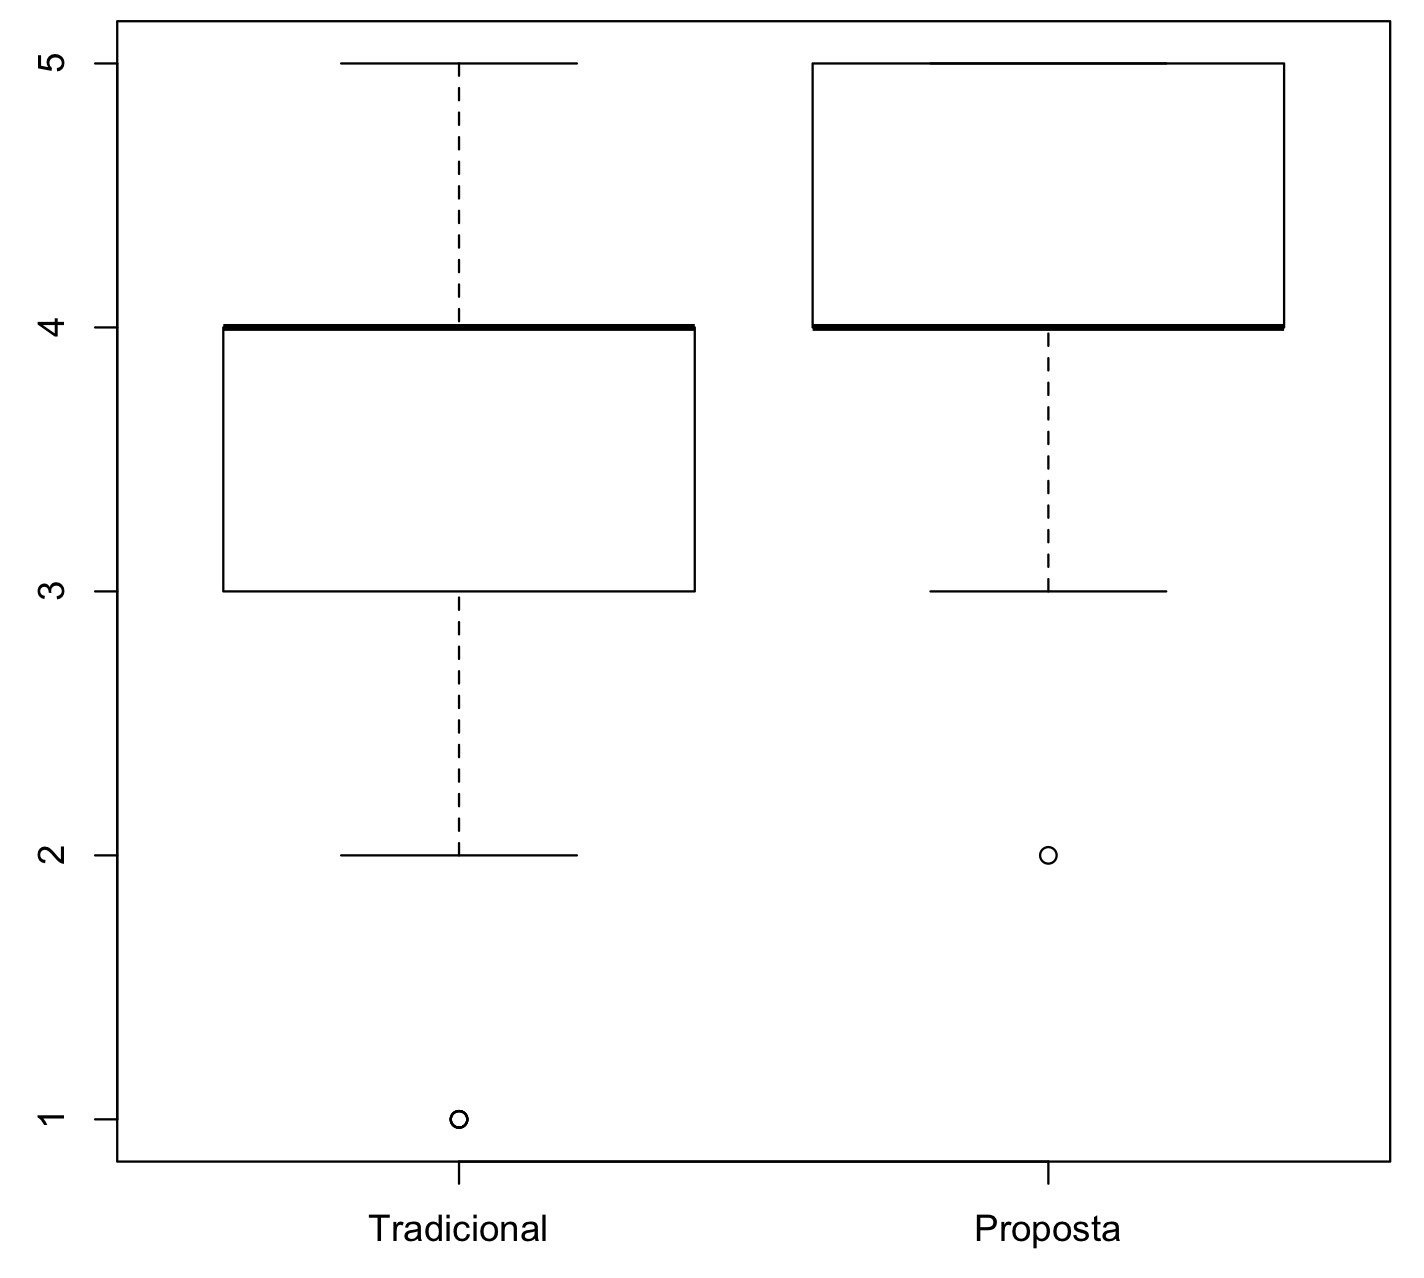
\includegraphics[scale=0.4]{./Figuras/questao12-boxplot.png}
  \end{center}
  \legend{Fonte: O autor.}
\end{figure}

\begin{multicols}{2}

\noindent\textbf{Tradicional}\\
Min.   :1.0\\
1st Qu.:3.0\\
Median :4.0\\
Mean   :3.4\\
3rd Qu.:4.0\\
Max.   :5.0\\
\columnbreak

\noindent\textbf{Proposta}\\
Min.   :2.00\\
1st Qu.:4.00\\
Median :4.00\\
Mean   :4.12\\
3rd Qu.:5.00\\
Max.   :5.00
\end{multicols}

Wilcoxon rank sum test with continuity correction

\noindent
data:  $data\_12\_tradicional$ and $data\_12\_proposta$\\
W = 240, p-value = 0.01513\\
alternative hypothesis: true location shift is not equal to 0

\textbf{Resultado: Aceita a hipótese alternativa - Com diferença significativa}

\newpage
\textbf{Questão 13: No geral, estou satisfeito com o sistema de recomendação.}

\begin{figure}[htb]
  \caption{\label{fig:questao13-boxplot}Boxplot da questão 13}
  \begin{center}
      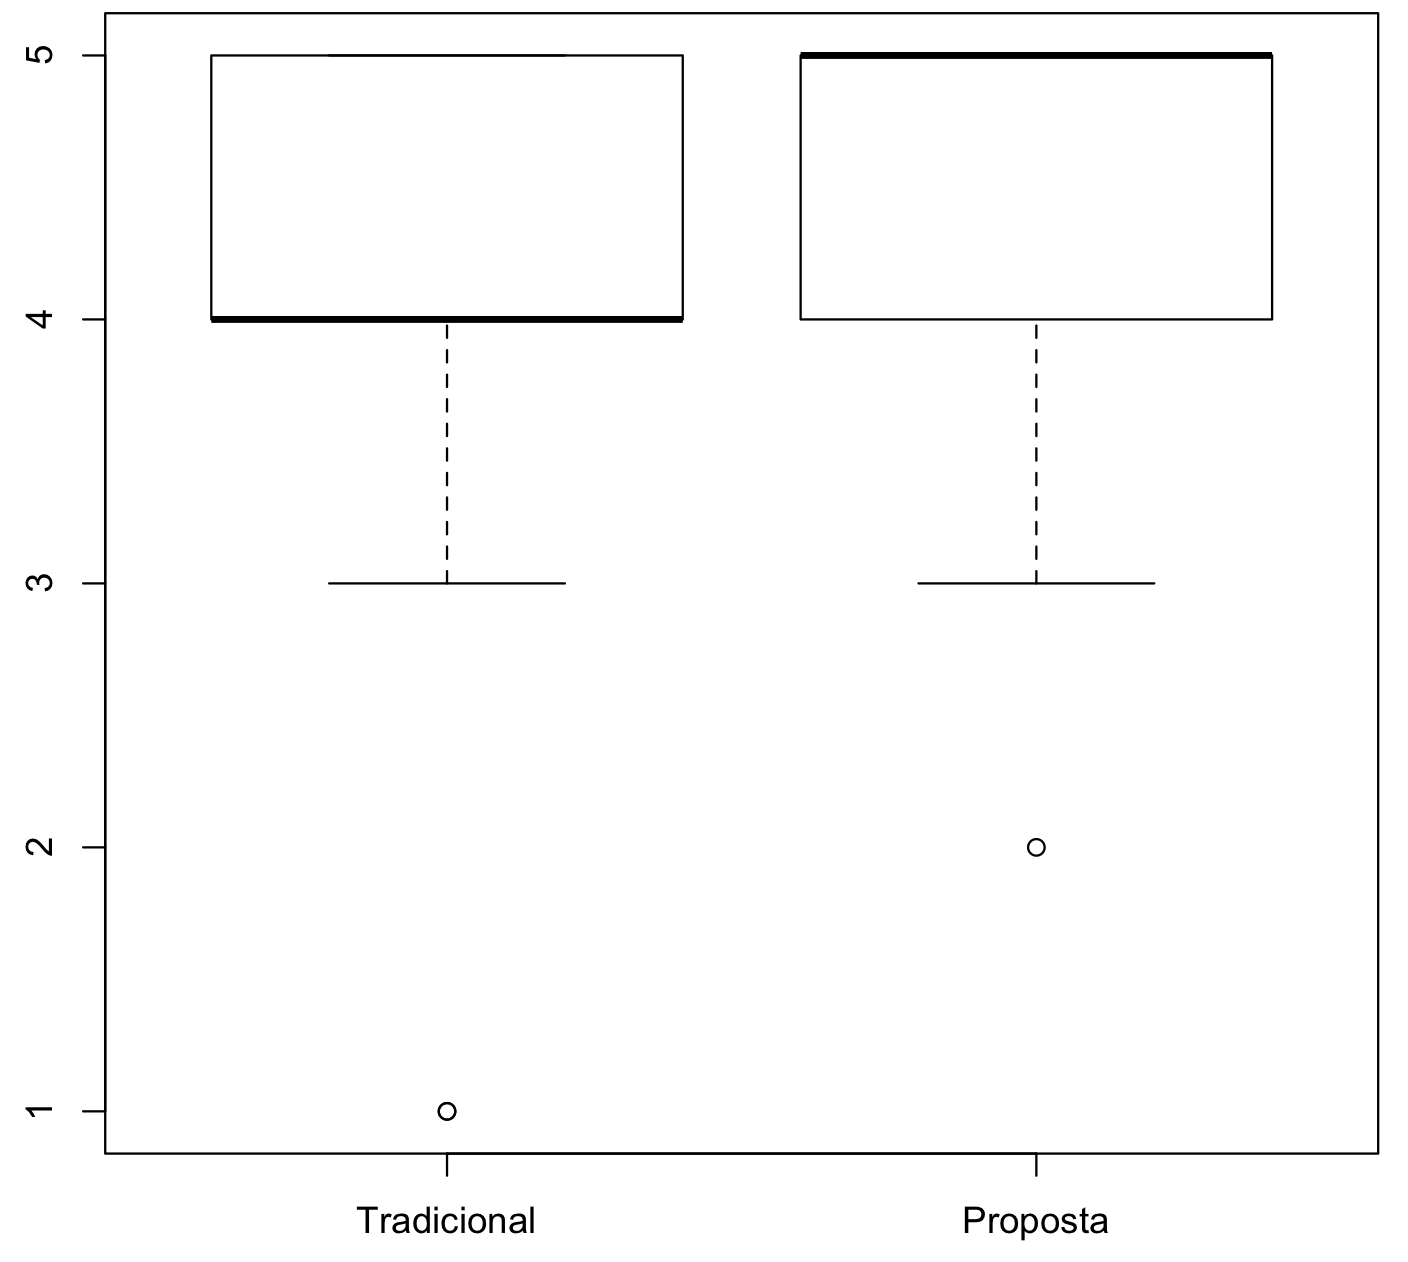
\includegraphics[scale=0.4]{./Figuras/questao13-boxplot.png}
  \end{center}
  \legend{Fonte: O autor.}
\end{figure}

\begin{multicols}{2}

\noindent\textbf{Tradicional}\\
Min.   :1\\
1st Qu.:4\\
Median :4\\
Mean   :4\\
3rd Qu.:5\\
Max.   :5\\
\columnbreak

\noindent\textbf{Proposta}\\
Min.   :2.000\\
1st Qu.:4.000\\
Median :5.000\\
Mean   :4.308\\
3rd Qu.:5.000\\
Max.   :5.000
\end{multicols}

Wilcoxon rank sum test with continuity correction

\noindent
data:  $data\_13\_tradicional$ and $data\_13\_proposta$\\
W = 356.5, p-value = 0.2388\\
alternative hypothesis: true location shift is not equal to 0

\end{apendicesenv}

% ----------------------------------------------------------
% Anexos
% ----------------------------------------------------------
\begin{anexosenv}
  % Imprime uma página indicando o início dos anexos
  \partanexos

  \chapter{60 Questões do Framework de Avaliação de Sistemas de Recomendação ResQue}\label{ane:questoes-framework}

\section{Quality of Recommended Items}

\subsection{Accuracy}

\begin{itemize}
\item The items recommended to me matched my interests.*
\item The recommender gave me good suggestions.
\item I am not interested in the items recommended to me (reverse scale).
\end{itemize}

\subsection{Relative Accuracy}

\begin{itemize}
\item The recommendation I received better fits my interests than what I may receive from a friend.
\item A recommendation from my friends better suits my interests than the recommendation from this system (reverse scale).
\end{itemize}

\subsection{Familiarity}

\begin{itemize}
\item Some of the recommended items are familiar to me.
\item I am not familiar with the items that were recommended to me (reverse scale).
\end{itemize}

\subsection{Attractiveness}

\begin{itemize}
\item The items recommended to me are attractive.
\end{itemize}

\subsection{Enjoyability}

\begin{itemize}
\item I enjoyed the items recommended to me.
\end{itemize}

\subsection{Novelty}

\begin{itemize}
\item The items recommended to me are novel and interesting.*
\item The recommender system is educational.
\item The recommender system helps me discover new products.
\item I could not find new items through the recommender (reverse scale).
\end{itemize}

\subsection{Diversity}

\begin{itemize}
\item The items recommended to me are diverse.*
\item The items recommended to me are similar to each other (reverse scale).*
\end{itemize}

\subsection{Context Compatibility}

\begin{itemize}
\item I was only provided with general recommendations.
\item The items recommended to me took my personal context requirements into consideration.
\item The recommendations are timely.
\end{itemize}

\section{Interaction Adequacy}

\begin{itemize}
\item The recommender provides an adequate way for me to express my preferences.
\item The recommender provides an adequate way for me to revise my preferences.
\item The recommender explains why the products are recommended to me.*
\end{itemize}

\section{Interface Adequacy}

\begin{itemize}
\item The recommender’s interface provides sufficient information.
\item The information provided for the recommended items is sufficient for me.
\item The labels of the recommender interface are clear and adequate.
\item The layout of the recommender interface is attractive and adequate.*
\end{itemize}

\section{Perceived Ease of Use}

\subsection{Ease of Initial Learning}

\begin{itemize}
\item I became familiar with the recommender system very quickly.
\item I easily found the recommended items.
\item Looking for a recommended item required too much effort (reverse scale).
\end{itemize}

\subsection{Ease of Preference Elicitation}

\begin{itemize}
\item I found it easy to tell the system about my preferences.
\item It is easy to learn to tell the system what I like.
\item It required too much effort to tell the system what I like (reversed scale).
\end{itemize}

\subsection{Ease of Preference Revision}

\begin{itemize}
\item I found it easy to make the system recommend different things to me.
\item It is easy to train the system to update my preferences.
\item I found it easy to alter the outcome of the recommended items due to my preference changes.
\item It is easy for me to inform the system if I dislike/like the recommended item.
\item It is easy for me to get a new set of recommendations.
\end{itemize}

\subsection{Ease of Decision Making}

\begin{itemize}
\item Using the recommender to find what I like is easy.
\item I was able to take advantage of the recommender very quickly.
\item I quickly became productive with the recommender.
\item Finding an item to buy with the help of the recommender is easy.*
\item Finding an item to buy, even with the help of the recommender, consumes too much time.
\end{itemize}

\section{Perceived Usefulness}

\begin{itemize}
\item The recommended items effectively helped me find the ideal product.*
\item The recommended items influence my selection of products.
\item I feel supported to find what I like with the help of the recommender.*
\item I feel supported in selecting the items to buy with the help of the recommender.
\end{itemize}

\section{Control/Transparency}

\begin{itemize}
\item I feel in control of telling the recommender what I want.
\item I don’t feel in control of telling the system what I want.
\item I don’t feel in control of specifying and changing my preferences (reverse scale).
\item I understood why the items were recommended to me.
\item The system helps me understand why the items were recommended to me.
\item The system seems to control my decision process rather than me (reverse scale).
\end{itemize}

\section{Attitudes}

\begin{itemize}
\item Overall, I am satisfied with the recommender.*
\item I am convinced of the products recommended to me.*
\item I am confident I will like the items recommended to me. *
\item The recommender made me more confident about my selection/decision.
\item The recommended items made me confused about my choice (reverse scale).
\item The recommender can be trusted.
\end{itemize}

\section{Behavioral Intentions}

\subsection{Intention to Use the System}

\begin{itemize}
\item If a recommender such as this exists, I will use it to find products to buy.
\end{itemize}

\subsection{Continuance and Frequency}

\begin{itemize}
\item I will use this recommender again.*
\item I will use this type of recommender frequently.
\item I prefer to use this type of recommender in the future.
\end{itemize}

\subsection{Recommendation to Friends}

\begin{itemize}
\item I will tell my friends about this recommender.*
\end{itemize}

\subsection{Purchase Intention}

\begin{itemize}
\item I would buy the items recommended, given the opportunity.*
\end{itemize}

  \chapter{Desafios}\label{ane:desafios}

\noindent
\textbf{Desafio 1:} \\
\\
Qual é a resposta correta para as equações abaixo?\\
\\
a) 6 / 2 * (1 + 2) = ?\\
b) 7 + 8 * 0 - 2 = ?\\
c) 2 + 5 x 3 + 4 = ?\\
d) 2 + 2 + 2 * 0 = ?\\
e) 7 + 7 / 7 + 7 * 7 - 7 = ?\\
f) 12 / 2 * (6 - 7 + 4) * 2 = ?\\
\\
Por quê?\\
\\
\textbf{Desafio 2:} \\
\\
Observe a sequência: 2, 5, 10, 17, 26, ... \\
Escreva um programa que forneça o n-ésimo elemento desta sequência.\\
\\
Sabemos que não existe uma única forma de se resolver, e que cada pessoa pensa de maneira diferente. Compartilhe com os
outros participantes, através do fórum de discussões, como você desvendou a sequência, e qual estratégia você usou para
resolvê-la.\\
\\
\textbf{Desafio 3:} \\
\\
Crie uma calculadora de tempo. Por exemplo, calcular a diferença entre 3:15:33 (3 horas : 15 minutos : 33 segundos) e
17:28:22. A resposta também deve ser em horas:minutos:segundos.\\
\\
Compartilhe através do fórum a sua solução, e qual estratégia usou para escrever o programa.\\

\end{anexosenv}

\end{document}